\chapter{Veto efficiency studies}\label{chap:VetoEfficiency}
A WIMP scatter should only deposit a small amount of energy (few~keV) within the LXe volume of the experiment without any simultaneous energy deposit in the surrounding materials. Neutrons produced through radioactive decays within detector materials would mimic a WIMP interaction when they scatter off Xe atoms. Active material surrounding the central LXe volume also permits assessment of the local radioactivity environment, and thus to infer additional information on the backgrounds in the WIMP search region. A persuasive WIMP discovery will require excellent understanding of all background sources, which is best done through the characterization of those sources in situ. Efficiency of the veto systems in the detection of the radiation produced by the backgrounds should be maximised whilst minimizing the impact of the veto selection on detector livetime in turn maximising the detector livetime available for the detection of WIMPs. \autoref{sec:VetoEff/simulation_improvements} describes the series of improvements to the detector simulation which were made prior to the WS2024 science run which aided the understanding of the response from the veto detector systems. The refinement of the veto selection algorithm is discussed alongside the impact that the veto selection had on the WS2024 result from \autoref{sec:VetoEff/VetoSelectionOptimisation} onwards.

\section{Simulation matching}\label{sec:VetoEff/simulation_improvements}
\subsection{Tuning the OD simulations}
\subsubsection{Geometry edits}\label{sec:VetoEff/GeometryEdits}
Prior to WS2024 result, there were a number of major differences between simulations and data in the Outer Detector. As such, an effort was made to correct this. The changes made were as follows:
\begin{enumerate}
	\item Spacing was added between the acrylic tanks to account for the gap seen during installation.
	\item Water was added to the foam volume which is between the OCV and acrylic tanks.
	\item The acrylic tanks were moved further away from the OCV; this matches what adding the gaps was supposed to solve.
\end{enumerate}

The water percentage of the foam was increased in 1\% steps, and the acrylic tanks were moved by 10~mm steps.
In the analysis of the different variations of simulations the percentage of water in the foam, and the outward movement of the acrylic tanks were looped over.
The `best' configuration of the simulation geometry changes was found to be 30mm and 6\% through matching the capture time of neutrons following single scatters in the active LXe volume. Additional details on the discrepancies between simulations and data with respect to neutron capture timing is shown in the subsequent subsection.
\begin{figure}[ht!]
	\centering
	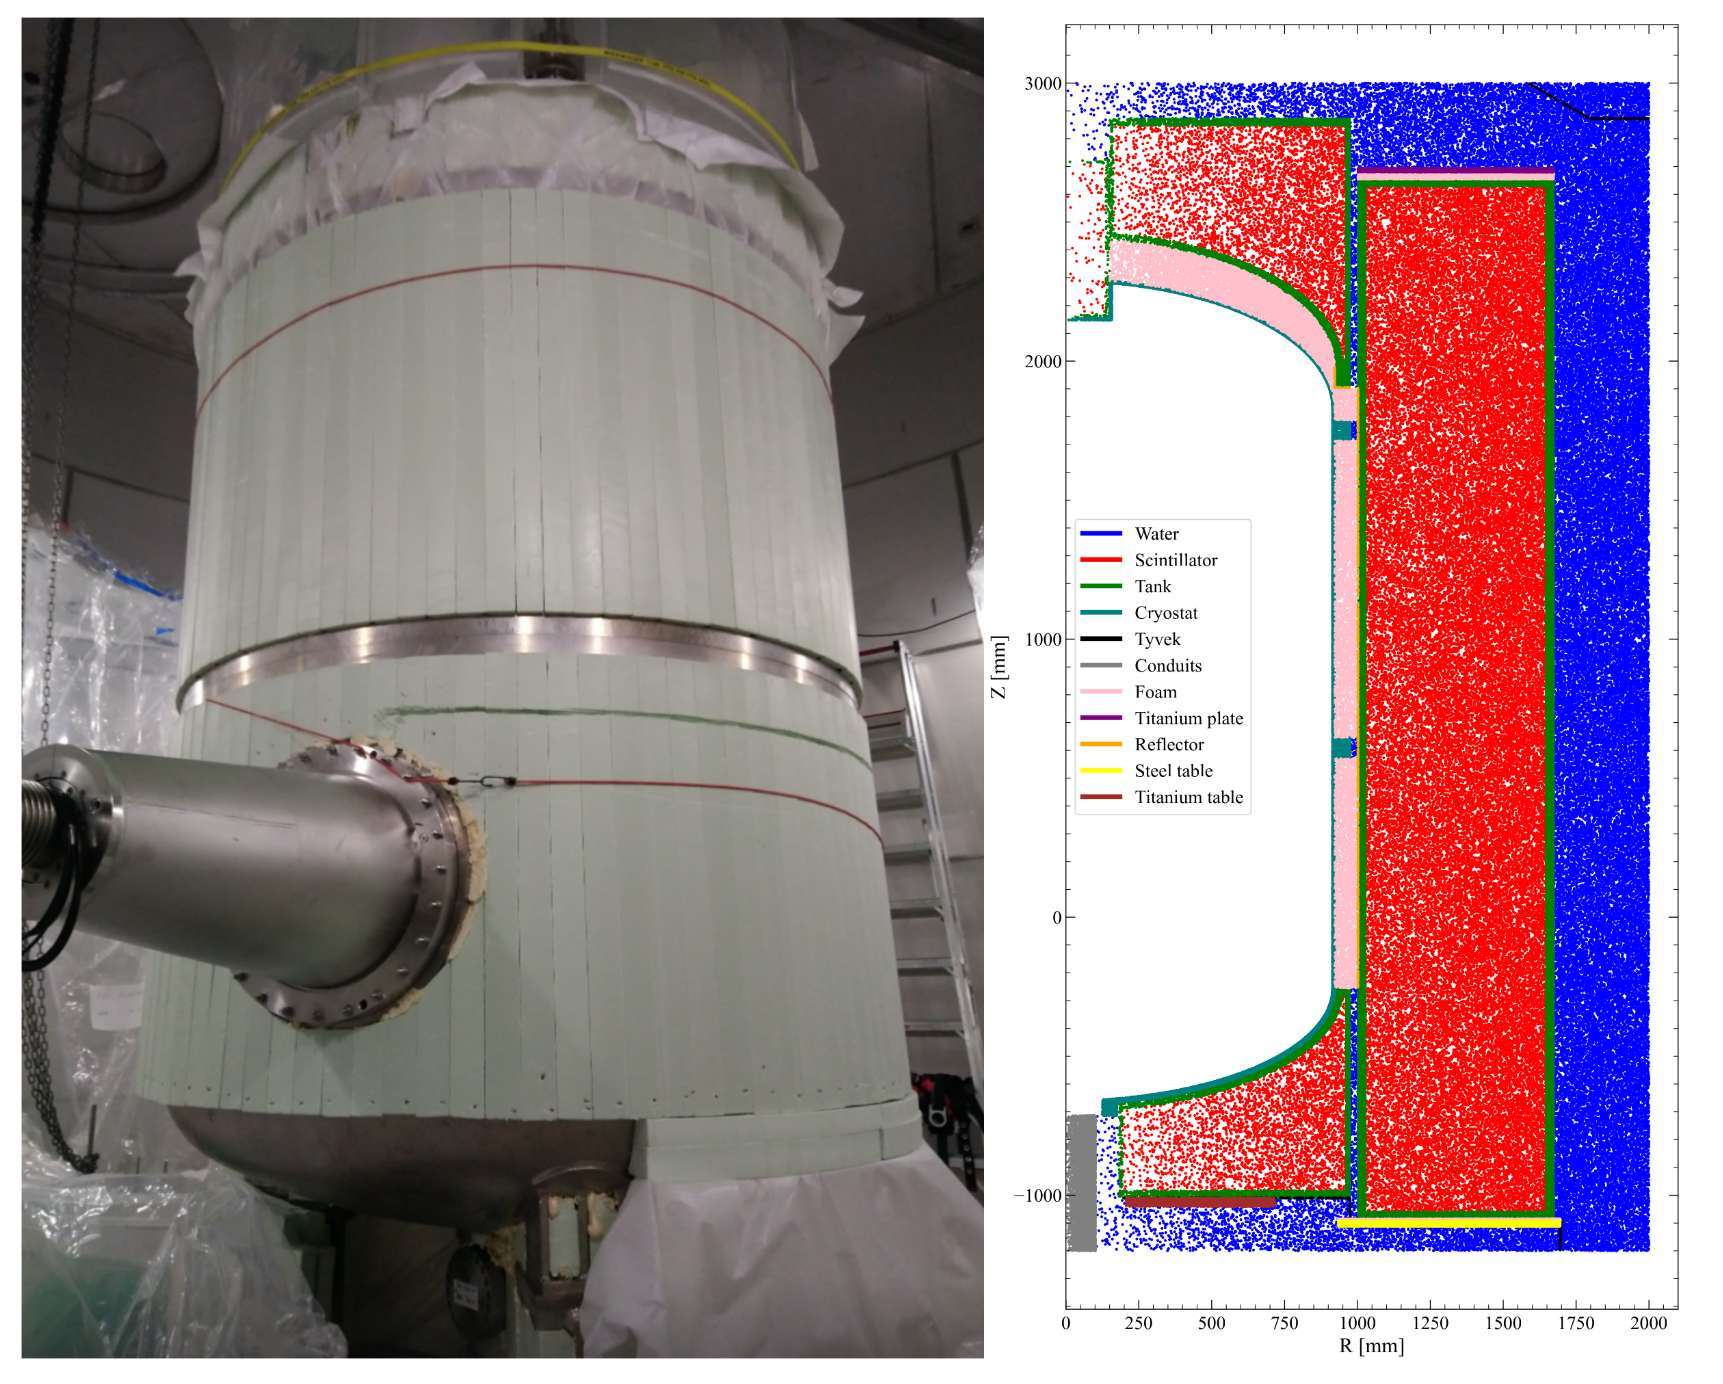
\includegraphics[width=0.9\textwidth]{figures/VetoEfficiency/FoamImgAndSimGeoTogether.png}
	\caption{Geometry in the simulation used for the WS2024 science run. \textbf{Left:} A photograph of the light green foam water displacer which resides between the acrylic tanks and the OCV. The water displacer was wrapped in a light reflector made from Tyvek. \textbf{Right:} A cross-section of the BACCARAT output. Geantinos were been passed through the simulation geometry, the $xyz$ position information and GEANT4 volumes were recorded to show the various volumes in the simulation.}
	\label{fig:VetoEff/od_geometry_for_sr3}
\end{figure}

\subsubsection{Neutron capture time}\label{sec:VetoEff/NCT}
Following the geometry changes discussed above, the neutron capture timing using AmLi was studied. Prior to the geometry changes, there was a distinct discrepancy between data and simulation when considering neutron capture timing following single scatters within the TPC. Initial skims of both data and simulation were made using ALPACA, selecting all events which were classified as single scatters by LZAP. OD pulse information was also skimmed considering 100~keV (24~phd), 200~keV (49~phd) and 1~MeV (251~phd) OD thresholds. The geometry was optimised for the 200~keV threshold associated with proton recoil of neutrons of hydrogen in the OD medium.
All possible configurations of the geometry modifications were visually examined to determine which variation of simulation matched the data. An example of the comparison plot can be seen in \autoref{fig:VetoEff/NC_AmLi_50mm7}, the "baseline simulation" was the initially configuration of the geometry prior to this study. All plots were examined side by side in a large scale canvas configuration seen in \autoref{fig:VetoEff/NC_Canvas}. It was found that from this study that 30~mm~to~50~mm movement of the SATs alongside 5\%~to~7\% increase in the percentage of water in the foam provides the best agreement between data and simulation at a 200~keV threshold.
\begin{figure}[!ht]
	\centering
	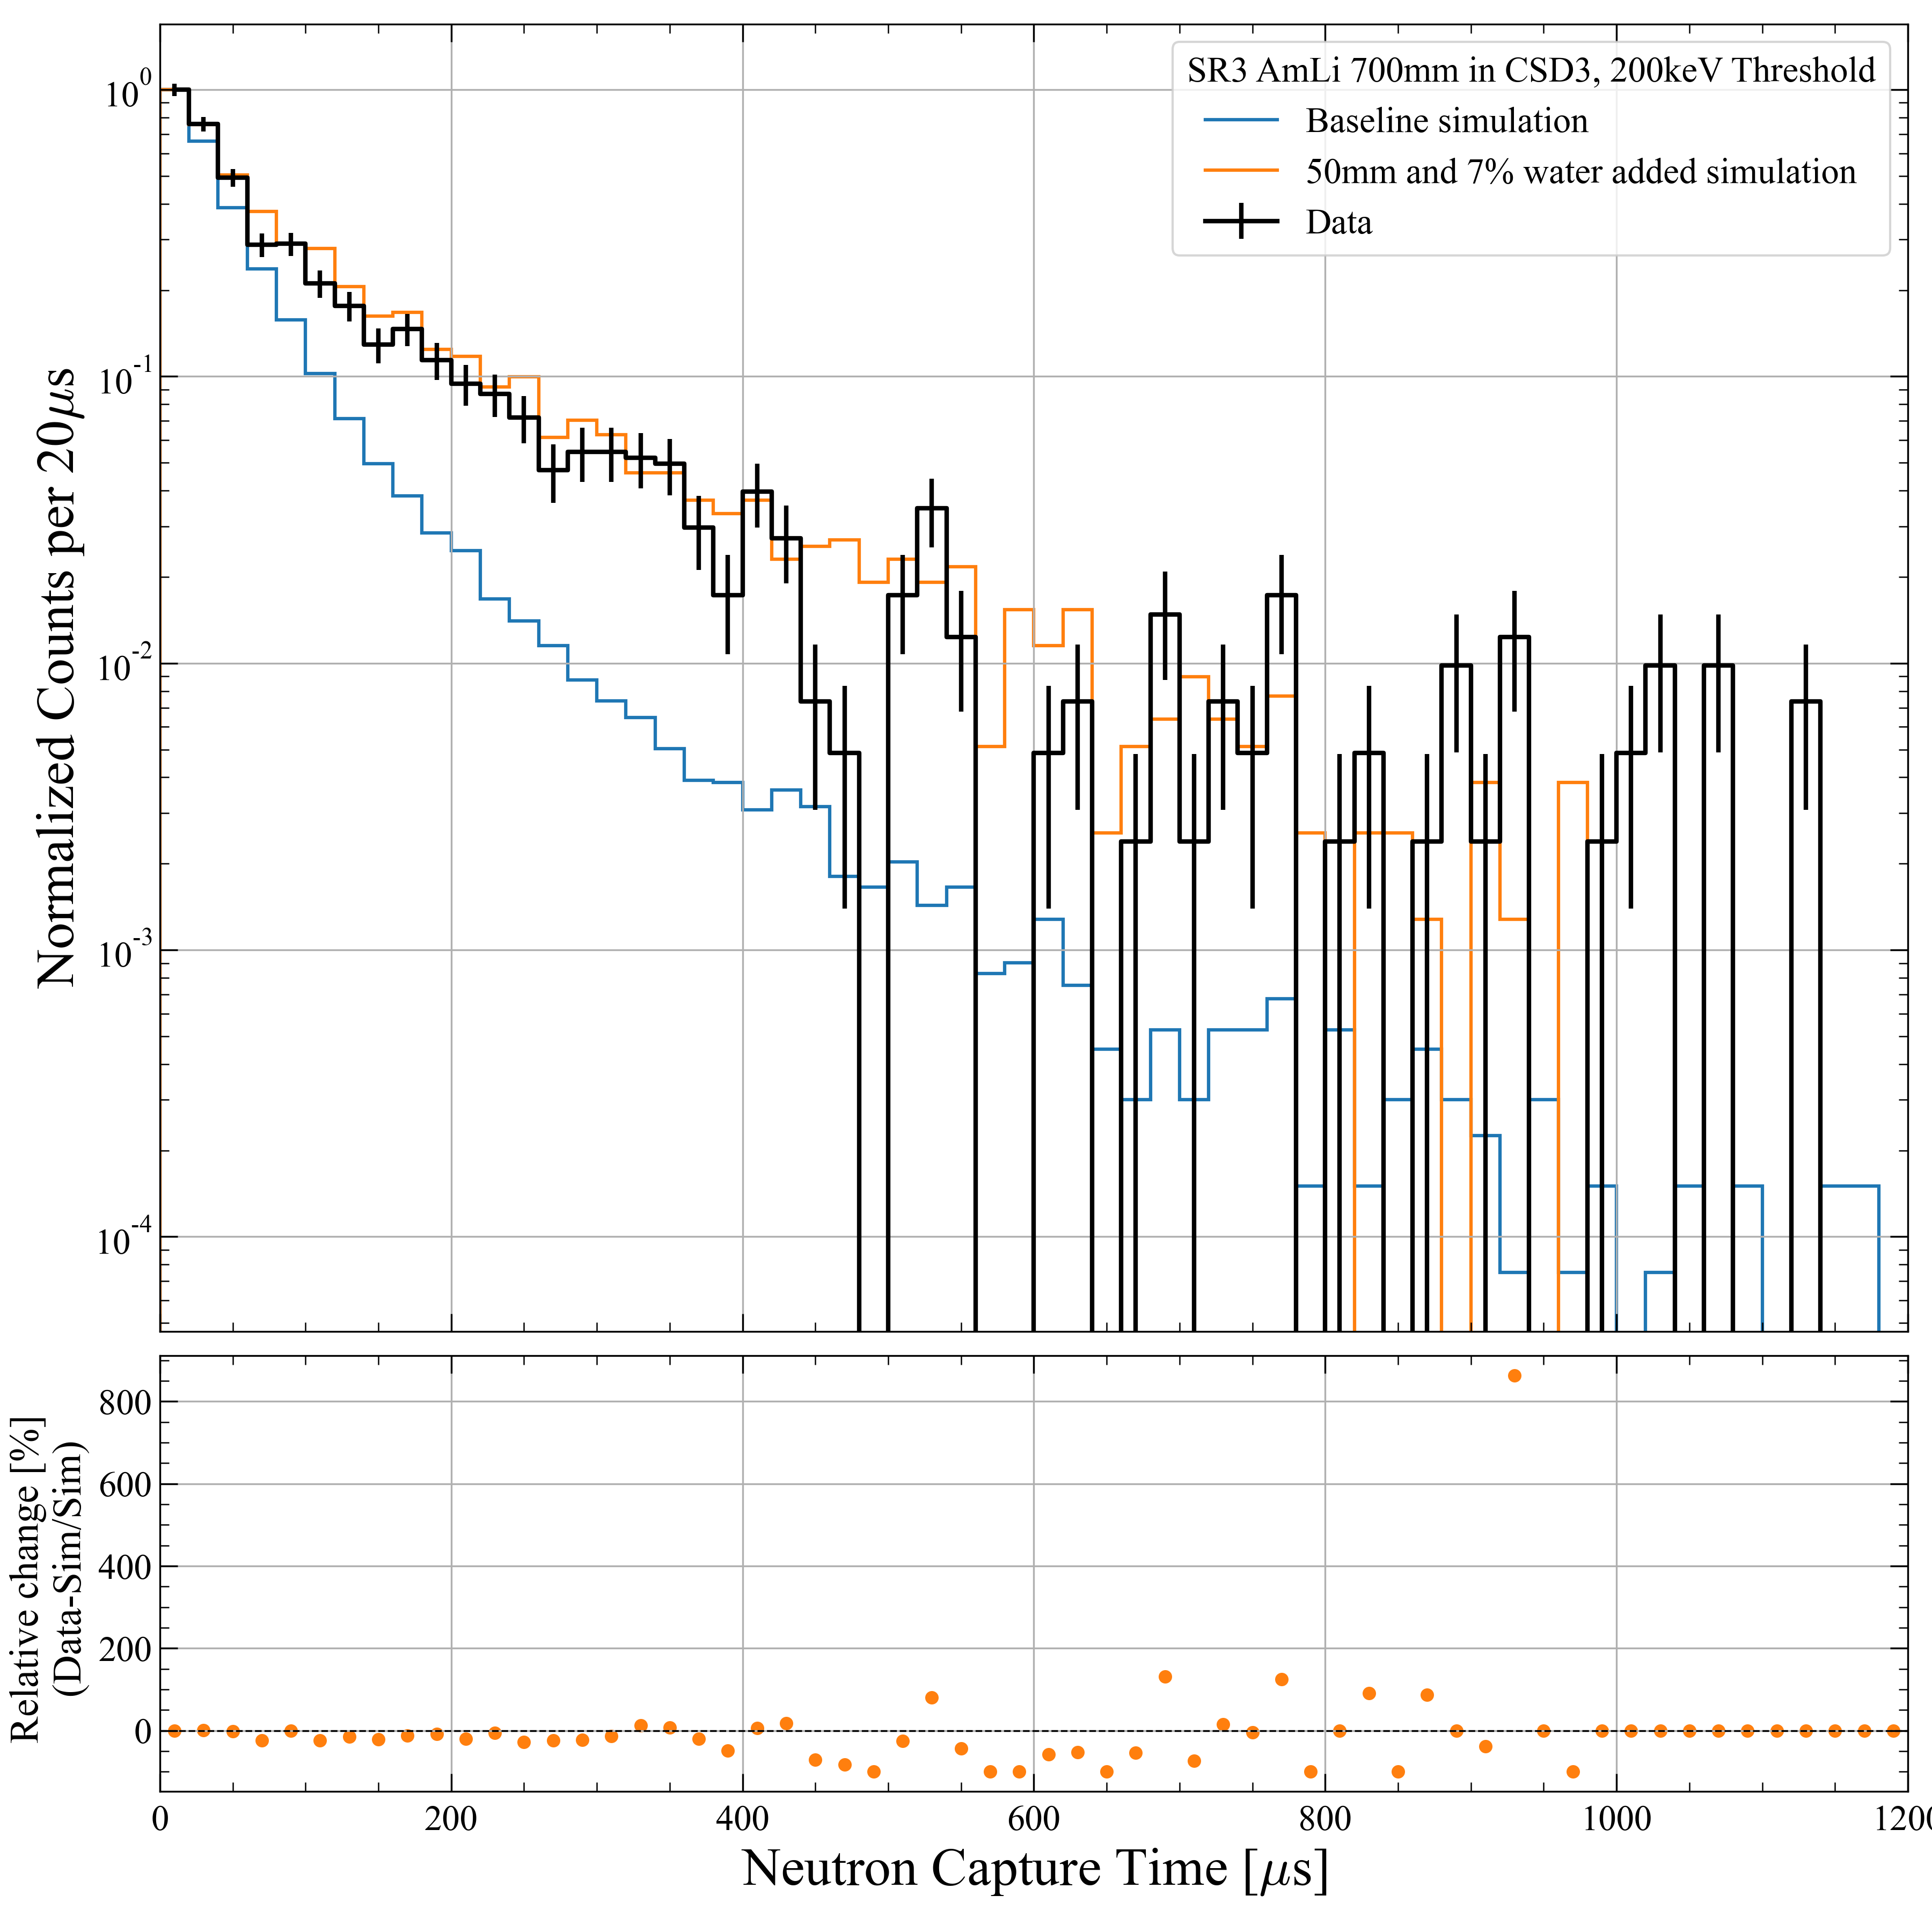
\includegraphics[width=0.8\linewidth]{figures/VetoEfficiency/movedSAT50mm_7percentWater_AmLi_CSD3_Z700mm_200keV_Ratio.png}
	\caption{An example of the plot used to compare neutron capture timing in data with the baseline simulation and the modified simulation. The relative change between data and simulation in each $20~\mu s$ bin was used to aid the visually examination across the $1200~\mu s$ window.}
	\label{fig:VetoEff/NC_AmLi_50mm7}
\end{figure}

\begin{sidewaysfigure}[ht!]
	\centering
	\includegraphics[width=\linewidth]{figures/VetoEfficiency/NCTiming_Canvas_700mm_AmLi.pdf}
	\caption{Large scale canvas of all possible simulation configurations. Each plot is similar in style to \autoref{fig:VetoEff/NC_AmLi_50mm7}. Here AmLi at 700mm in CSD3 has been shown as an example.}
	\label{fig:VetoEff/NC_Canvas}
\end{sidewaysfigure}


\section{Veto selection optimisation}\label{sec:VetoEff/VetoSelectionOptimisation}
In this section, details on how the Skin and OD cuts used in the WS2024 science run were created are defined. The Skin and OD veto cuts used in the WS2024 science run were based on those developed for the WS2022 science run, described in \cite{LZCollaboration:2024lux}.
The veto selection boils down to four cuts;
\begin{itemize}
	\item Skin-prompt: For tagging $\gamma$-rays in the Skin detector,
	\item OD-prompt: For tagging $\gamma$-rays and neutron proton recoils in the OD detector,
	\item Skin-delayed: For tagging $\gamma$-rays from post-neutron capture de-excitation,
	\item OD-delayed: For tagging $\gamma$-rays from post-neutron capture de-excitation.
\end{itemize}

Using WS2022 as a baseline, three studies were performed to adapt these cuts for WS2024;
\begin{enumerate}
	\item Determine the detector stability, to establish if the energy scale for the detectors has changed; using this the WS2022 cuts can simply be scaled for WS2024, and acts as a starting point.
	\item Implement a position correction to the OD.
	\item Perform cut optimisation based on the above studies.
\end{enumerate}
The cuts used for the vetoes were selected at the same time as AmLi neutron tagging efficiency calculation, and were set to maximise the tagging efficiency whilst reducing deadtime.

On a skim of the AmLi calibrations which pass the WS2024 core-cuts described in \autoref{tab:VetoEff/amli_efficiency_cuts}, the efficiency (described in \autoref{sec:VetoEff/efficiency}) was calculated with the pulse area, and coincidence thresholds of the Skin and OD varying in integer steps.
Heatmaps of the coincidence threshold vs. pulse area threshold vs. efficiency of each cut were produced, examples of these are shown in \autoref{fig:VetoEff/od_prompt_veto_heatmap} - \ref{fig:VetoEff/skin_delayed_veto_heatmap}.
For the delayed cuts, the veto time window was also varied, and heat maps of threshold vs. time window vs. efficiency were produced for a fixed coincidence. Heatmaps with dead time rather than efficiency were also produced. The dead time impact is discussed in greater detail \autoref{sec:VetoEff/DeadtimeStability}.

The windows for the prompt cuts were selected through the analysis of the DD and AmLi calibrations (the run numbers and the LZAP version are listed in \autoref{sec:VetoEff/efficiency}) and by measuring the time difference between the TPC single-scatter and OD and Skin pulses.
Both distributions for AmLi and DD are shown in \autoref{fig:VetoEff/veto_prompt_windows_OD} and \autoref{fig:VetoEff/veto_prompt_window_Skin} for the OD and Skin respectively.

Compiling the heat maps of efficiency and deadtime for a variety of veto windows, a choice of thresholds were chosen to maximise efficiency whilst minimising dead time. An example plot used to determine this is shown in \autoref{fig:VetoEff/veto_cut_optimisation}.
For the WS2024 science run, the approach of trying to maintain the efficiency of WS2022 veto of $\sim$~90\%, whilst reducing the livetime impact was taken.
From the heatmaps, it was determined that the efficiency could be matched to the veto efficiency achieved in the WS2022 science run, but with a much lower deadtime.
The final cuts for the WS2024 science run are shown in \autoref{tab:VetoEff/sr3_veto_cuts}, with the WS2022 selection included for comparison.

\begin{figure}[!ht]
	\centering
	\begin{subfigure}[b]{0.48\textwidth}
		\centering
		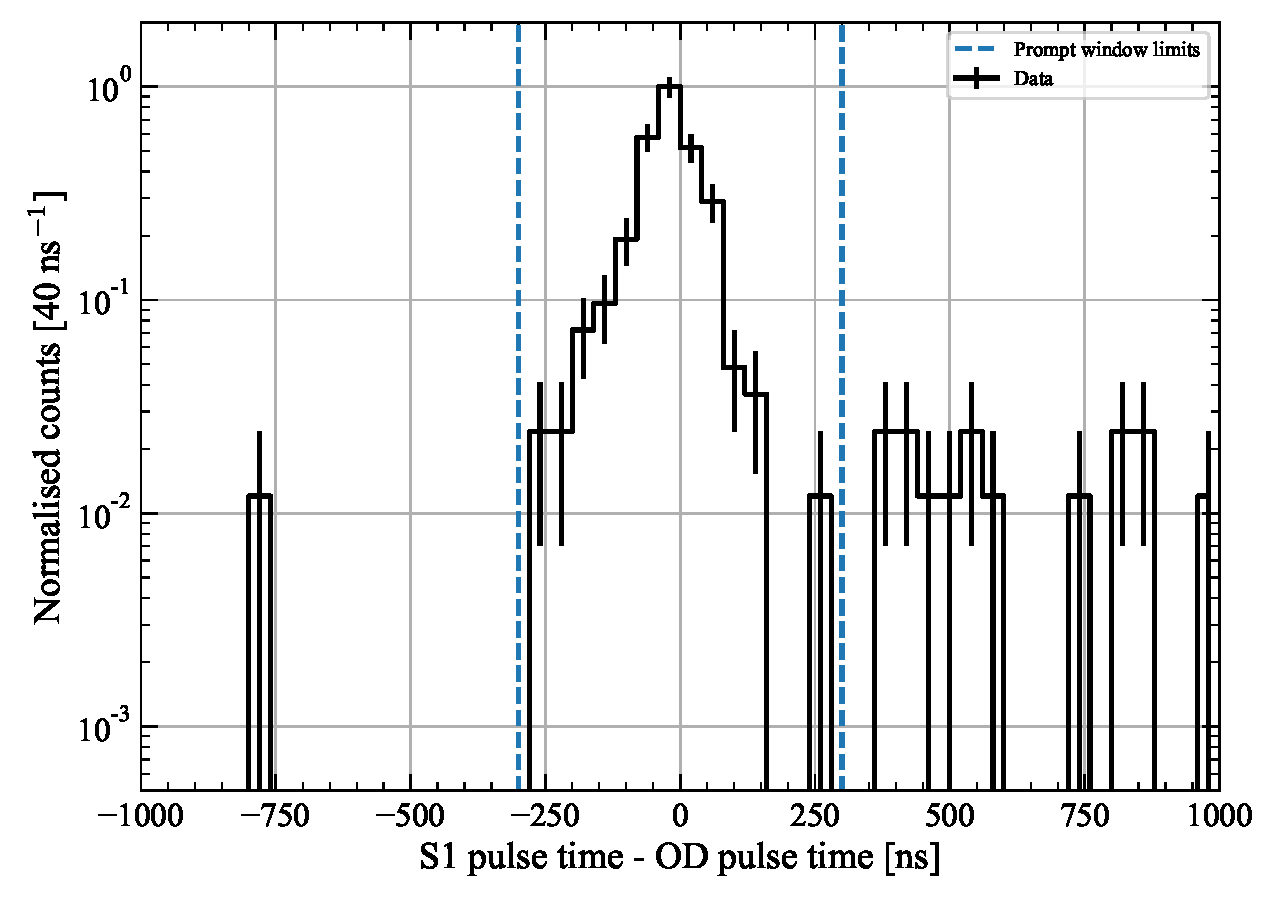
\includegraphics[width=\textwidth]{figures/VetoEfficiency/ODpromptWindowTiming_AmLi.pdf}
		\caption{Time difference (in ns) between TPC single-scatter and OD pulses using AmLi data.}
		\label{fig:VetoEff/od_prompt_window_AmLi}
	\end{subfigure}
	\hfill
	\begin{subfigure}[b]{0.48\textwidth}
		\centering
		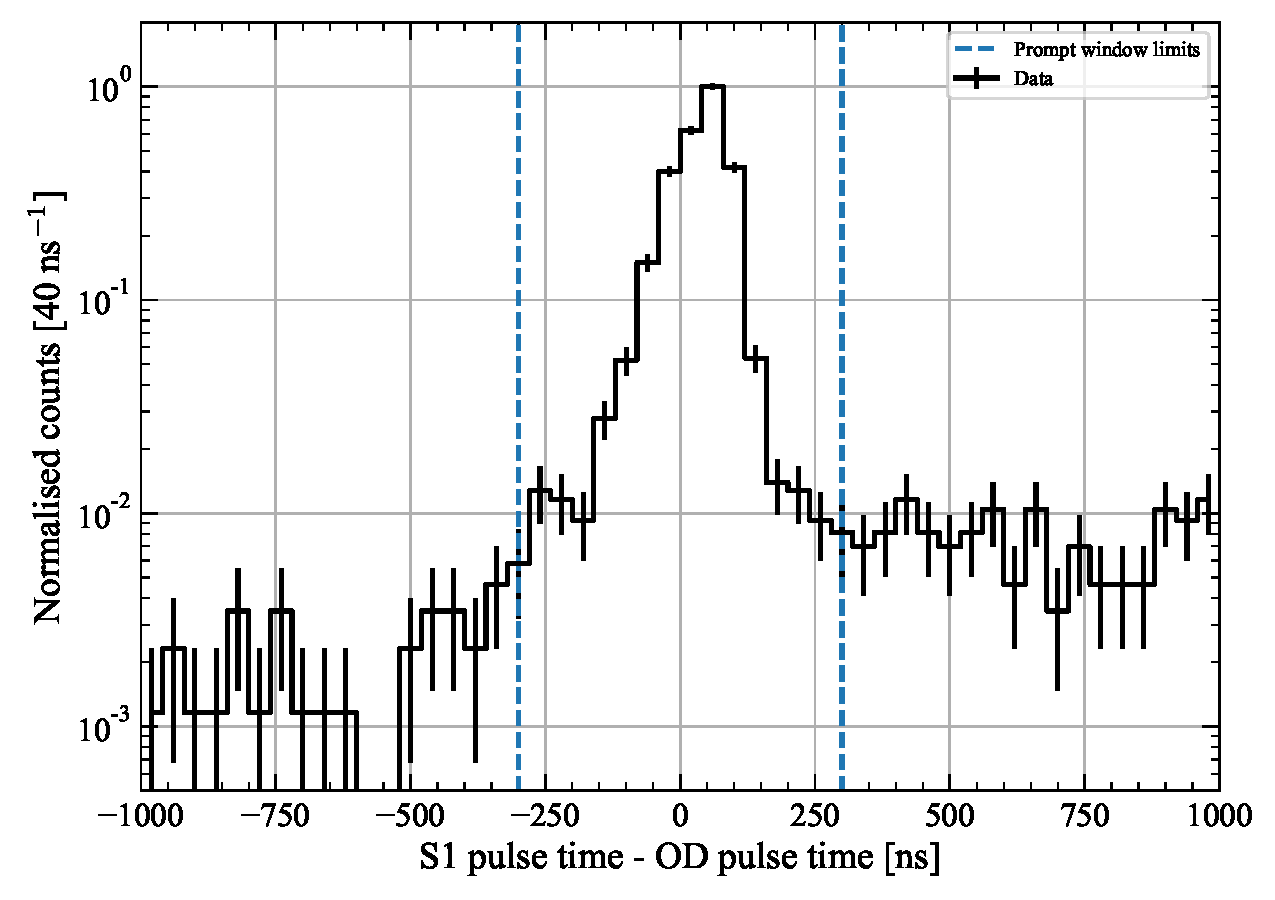
\includegraphics[width=\textwidth]{figures/VetoEfficiency/ODpromptWindowTiming_DD.pdf}
		\caption{Time difference (in ns) between TPC single-scatter and OD pulses using DD data.}
		\label{fig:VetoEff/od_prompt_window_DD}
	\end{subfigure}
	\caption{Time difference between TPC single-scatter and Veto pulses. To reduce the noise in the plot, a pulse requirement of greater than 5~phd and greater than 5~coincidence was been applied to the OD pulses. The vertical lines indicate the boundary of the WS2024 timing selection.}
	\label{fig:VetoEff/veto_prompt_windows_OD}
\end{figure}

\begin{figure}[!ht]
	\centering
	\begin{subfigure}[b]{0.48\textwidth}
		\centering
		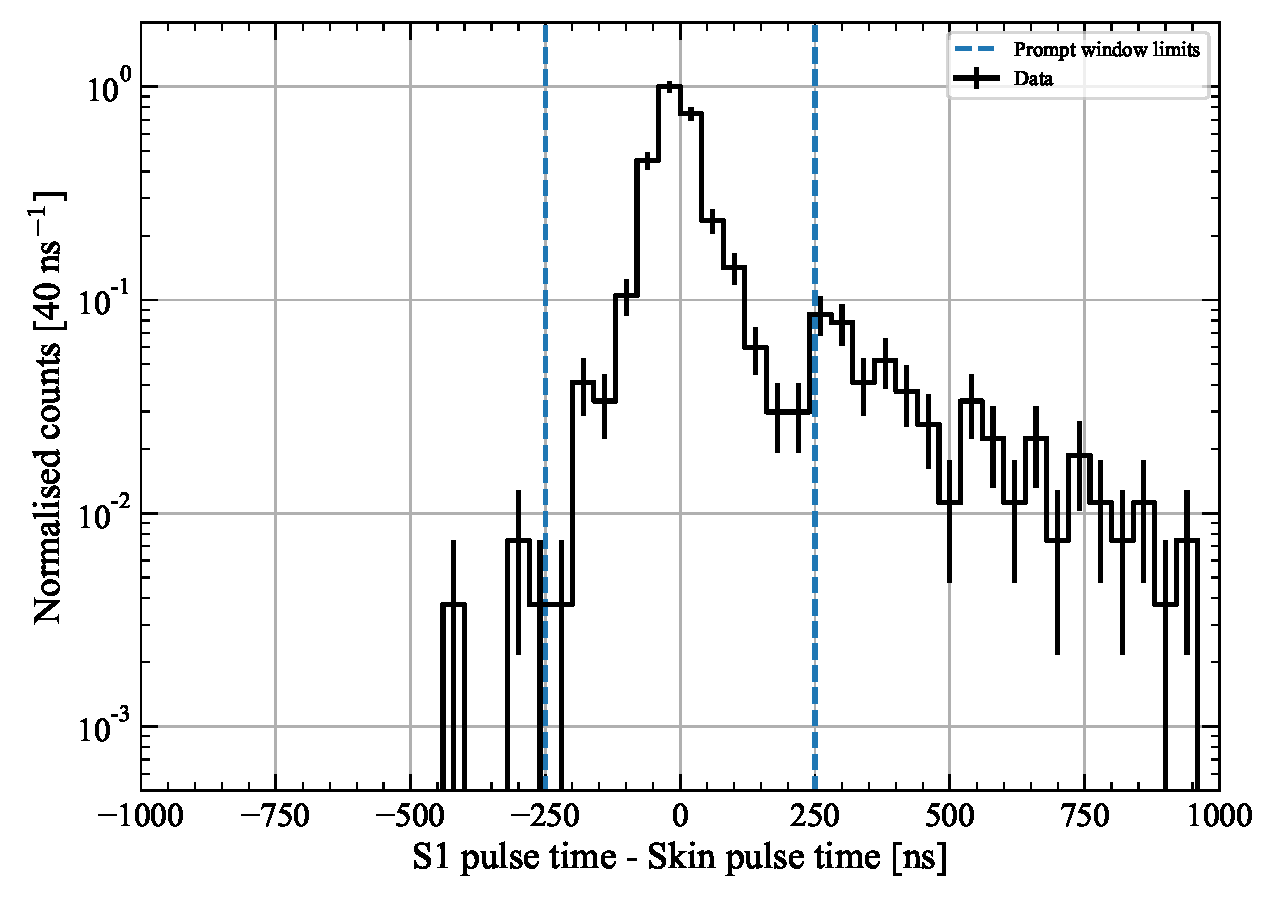
\includegraphics[width=\textwidth]{figures/VetoEfficiency/SkinpromptWindowTiming_AmLi.pdf}
		\caption{Time difference (in ns) between TPC single-scatter and OD pulses using AmLi data.}
		\label{fig:VetoEff/skin_prompt_window_AmLi}
	\end{subfigure}
	\hfill
	\begin{subfigure}[b]{0.48\textwidth}
		\centering
		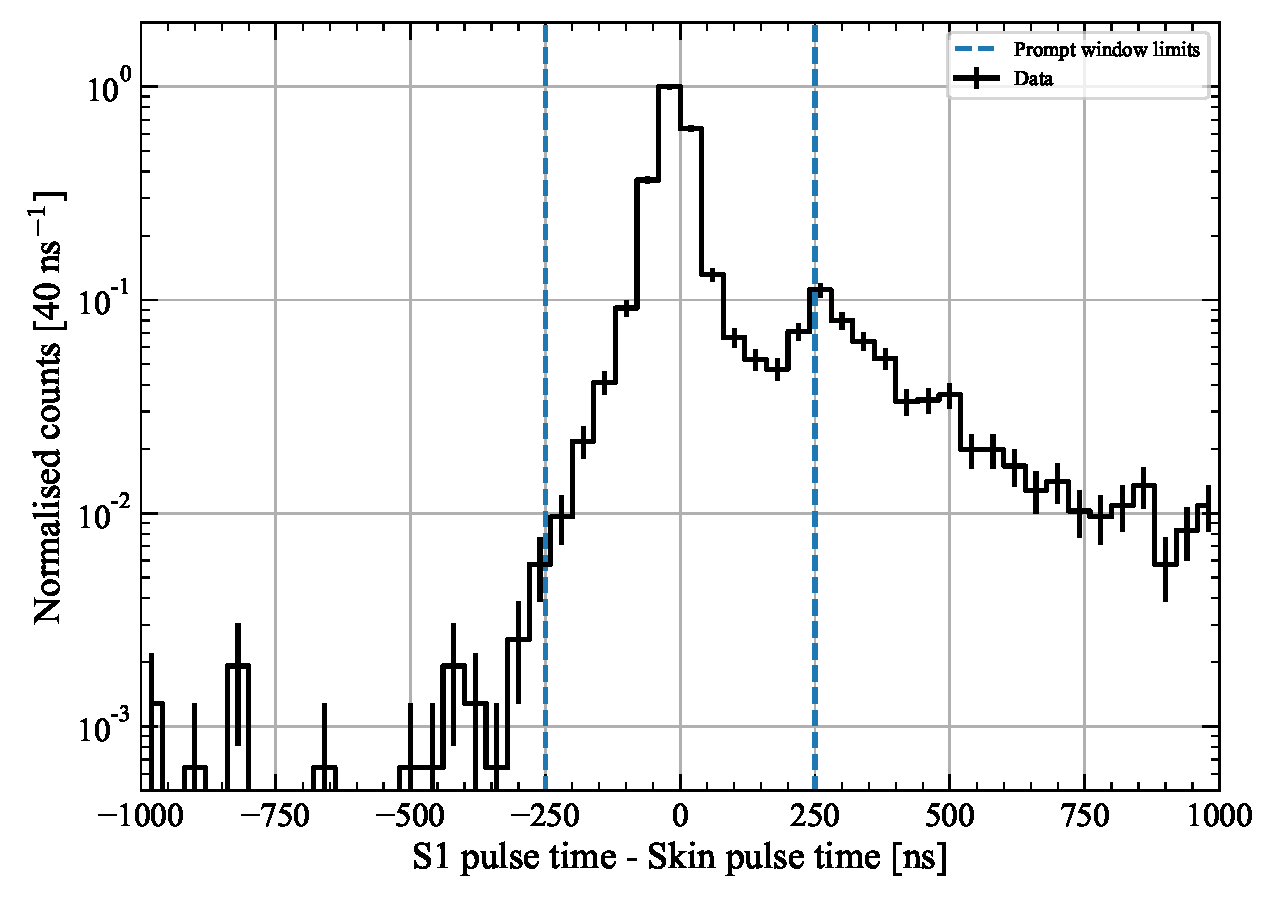
\includegraphics[width=\textwidth]{figures/VetoEfficiency/SkinpromptWindowTiming_DD.pdf}
		\caption{Time difference (in ns) between TPC single-scatter and OD pulses using DD data.}
		\label{fig:VetoEff/skin_prompt_window_DD}
	\end{subfigure}
	\caption{Time difference between TPC single-scatter and Veto pulses. To reduce the noise in the plot, a pulse requirement of greater than 2.5~phd and greater than 2~coincidence was been applied to the OD pulses. The vertical lines indicate the boundary of the WS2024 timing selection.}
	\label{fig:VetoEff/veto_prompt_window_Skin}
\end{figure}


\begin{sidewaysfigure}
	\centering
	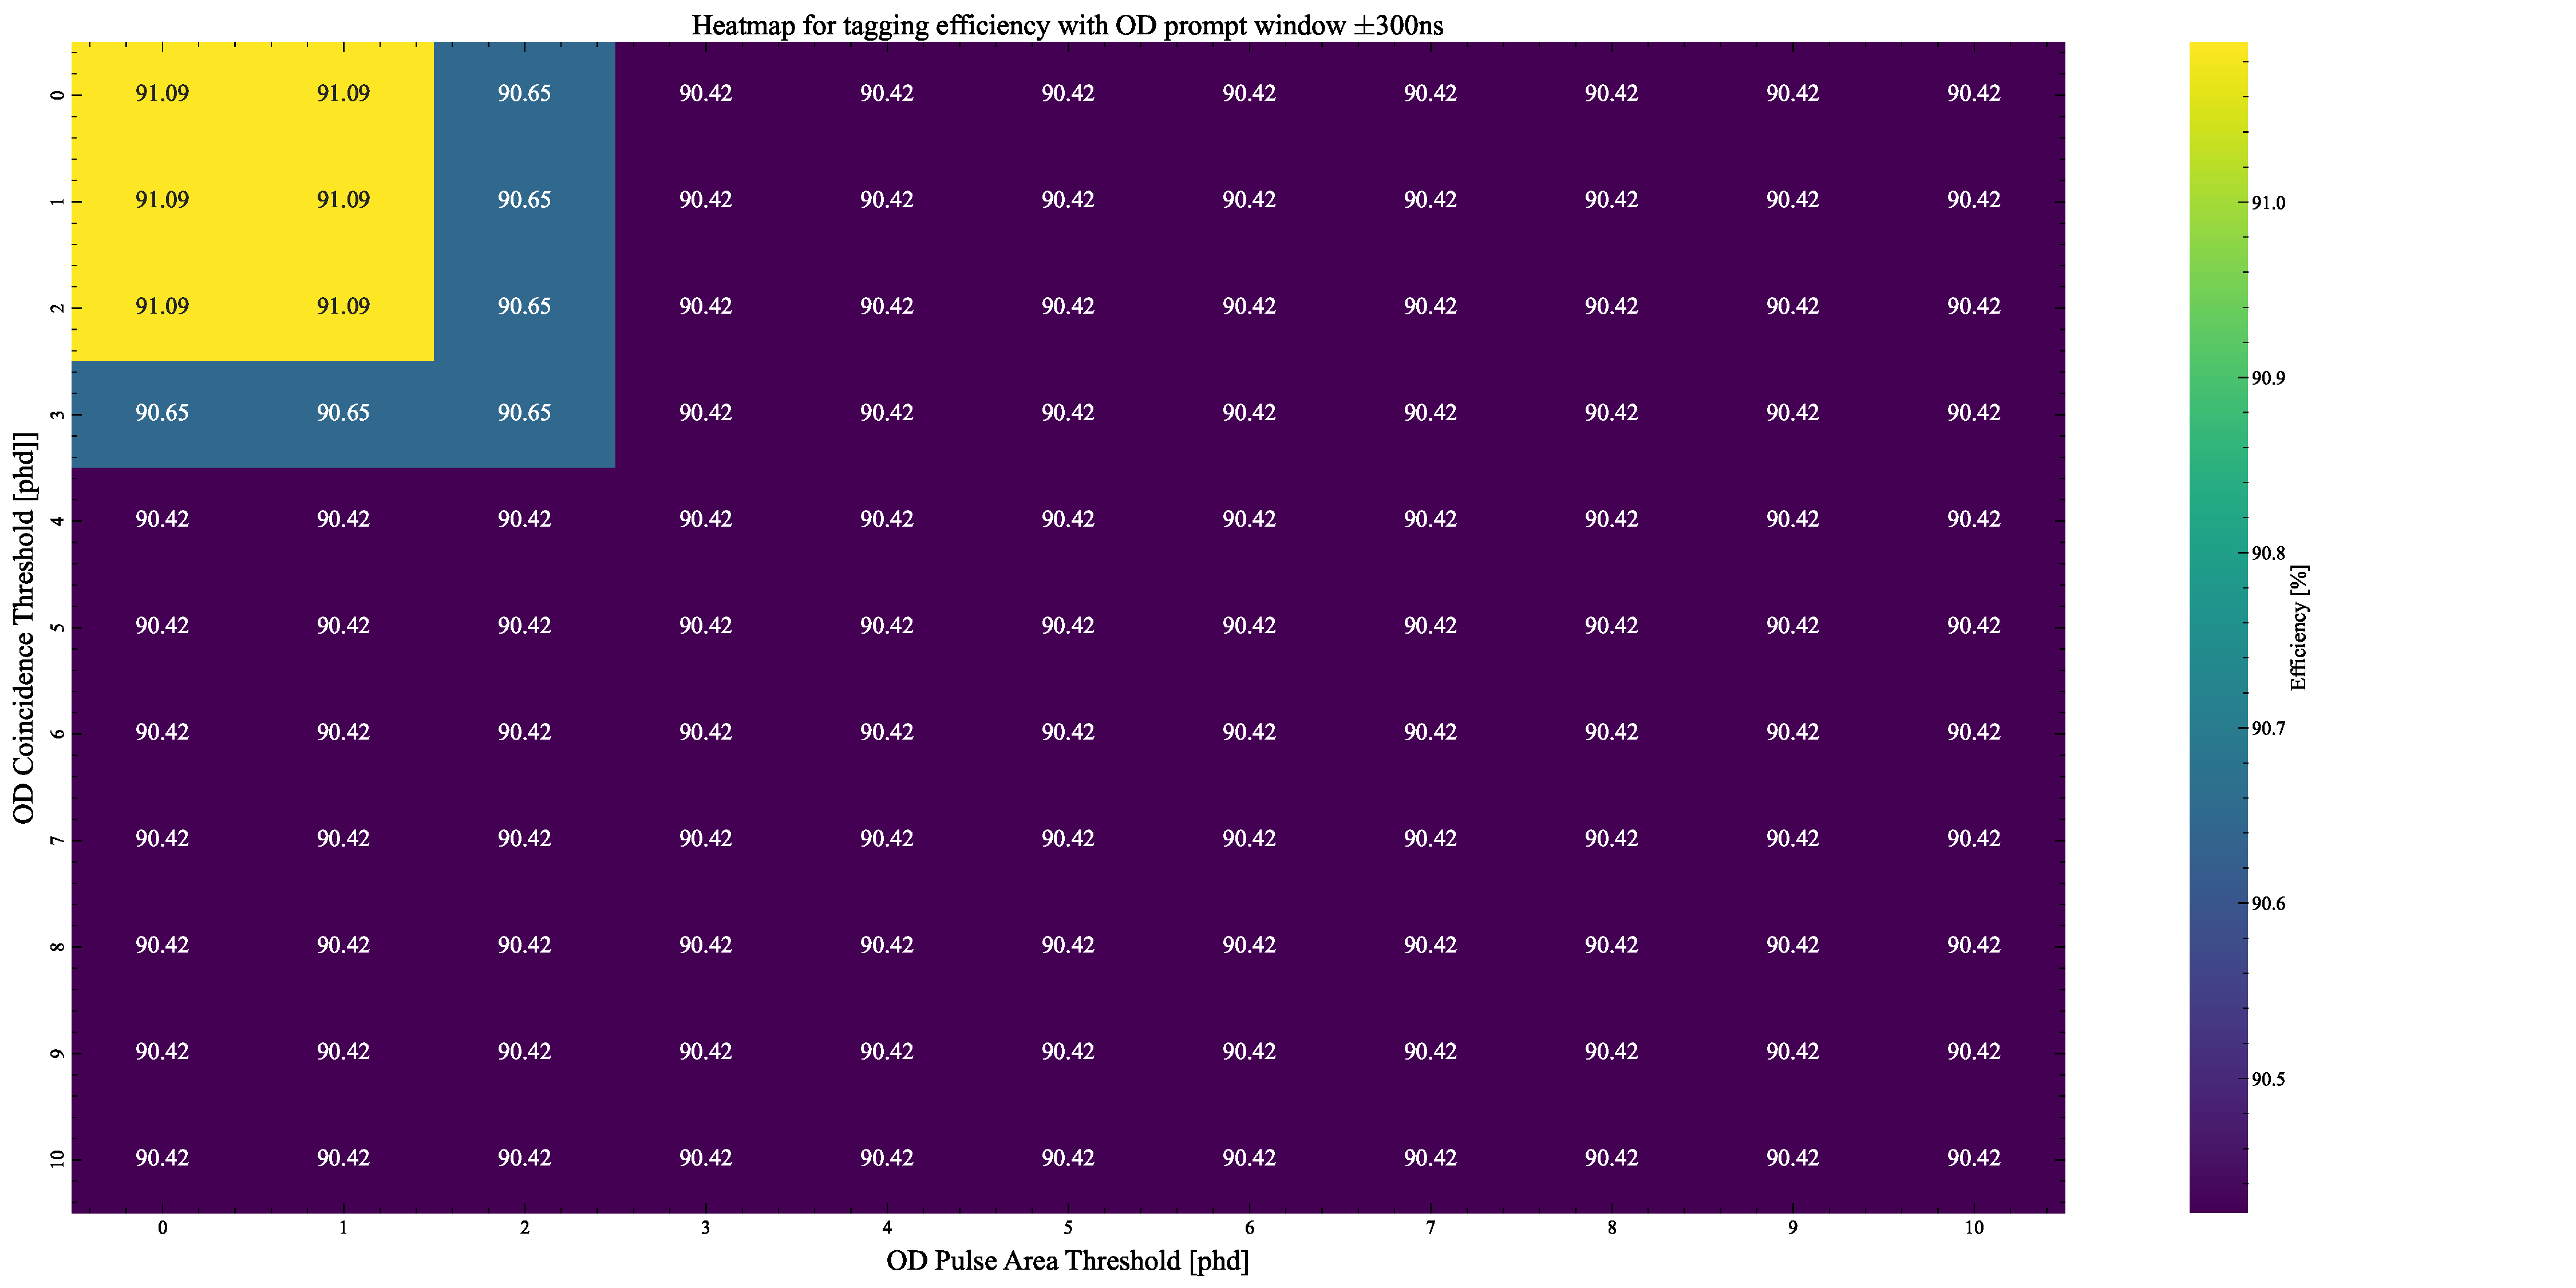
\includegraphics[width=\textwidth]{figures/VetoEfficiency/HeatmapODPACoinScanWindow600.pdf}
	\caption{OD Prompt heatmap.
		The z-axis shows the efficiency associated with a given pulse requirement.
		The veto time window considered is [-300, 300]ns.
	}
	\label{fig:VetoEff/od_prompt_veto_heatmap}
\end{sidewaysfigure}

\begin{sidewaysfigure}
	\centering
	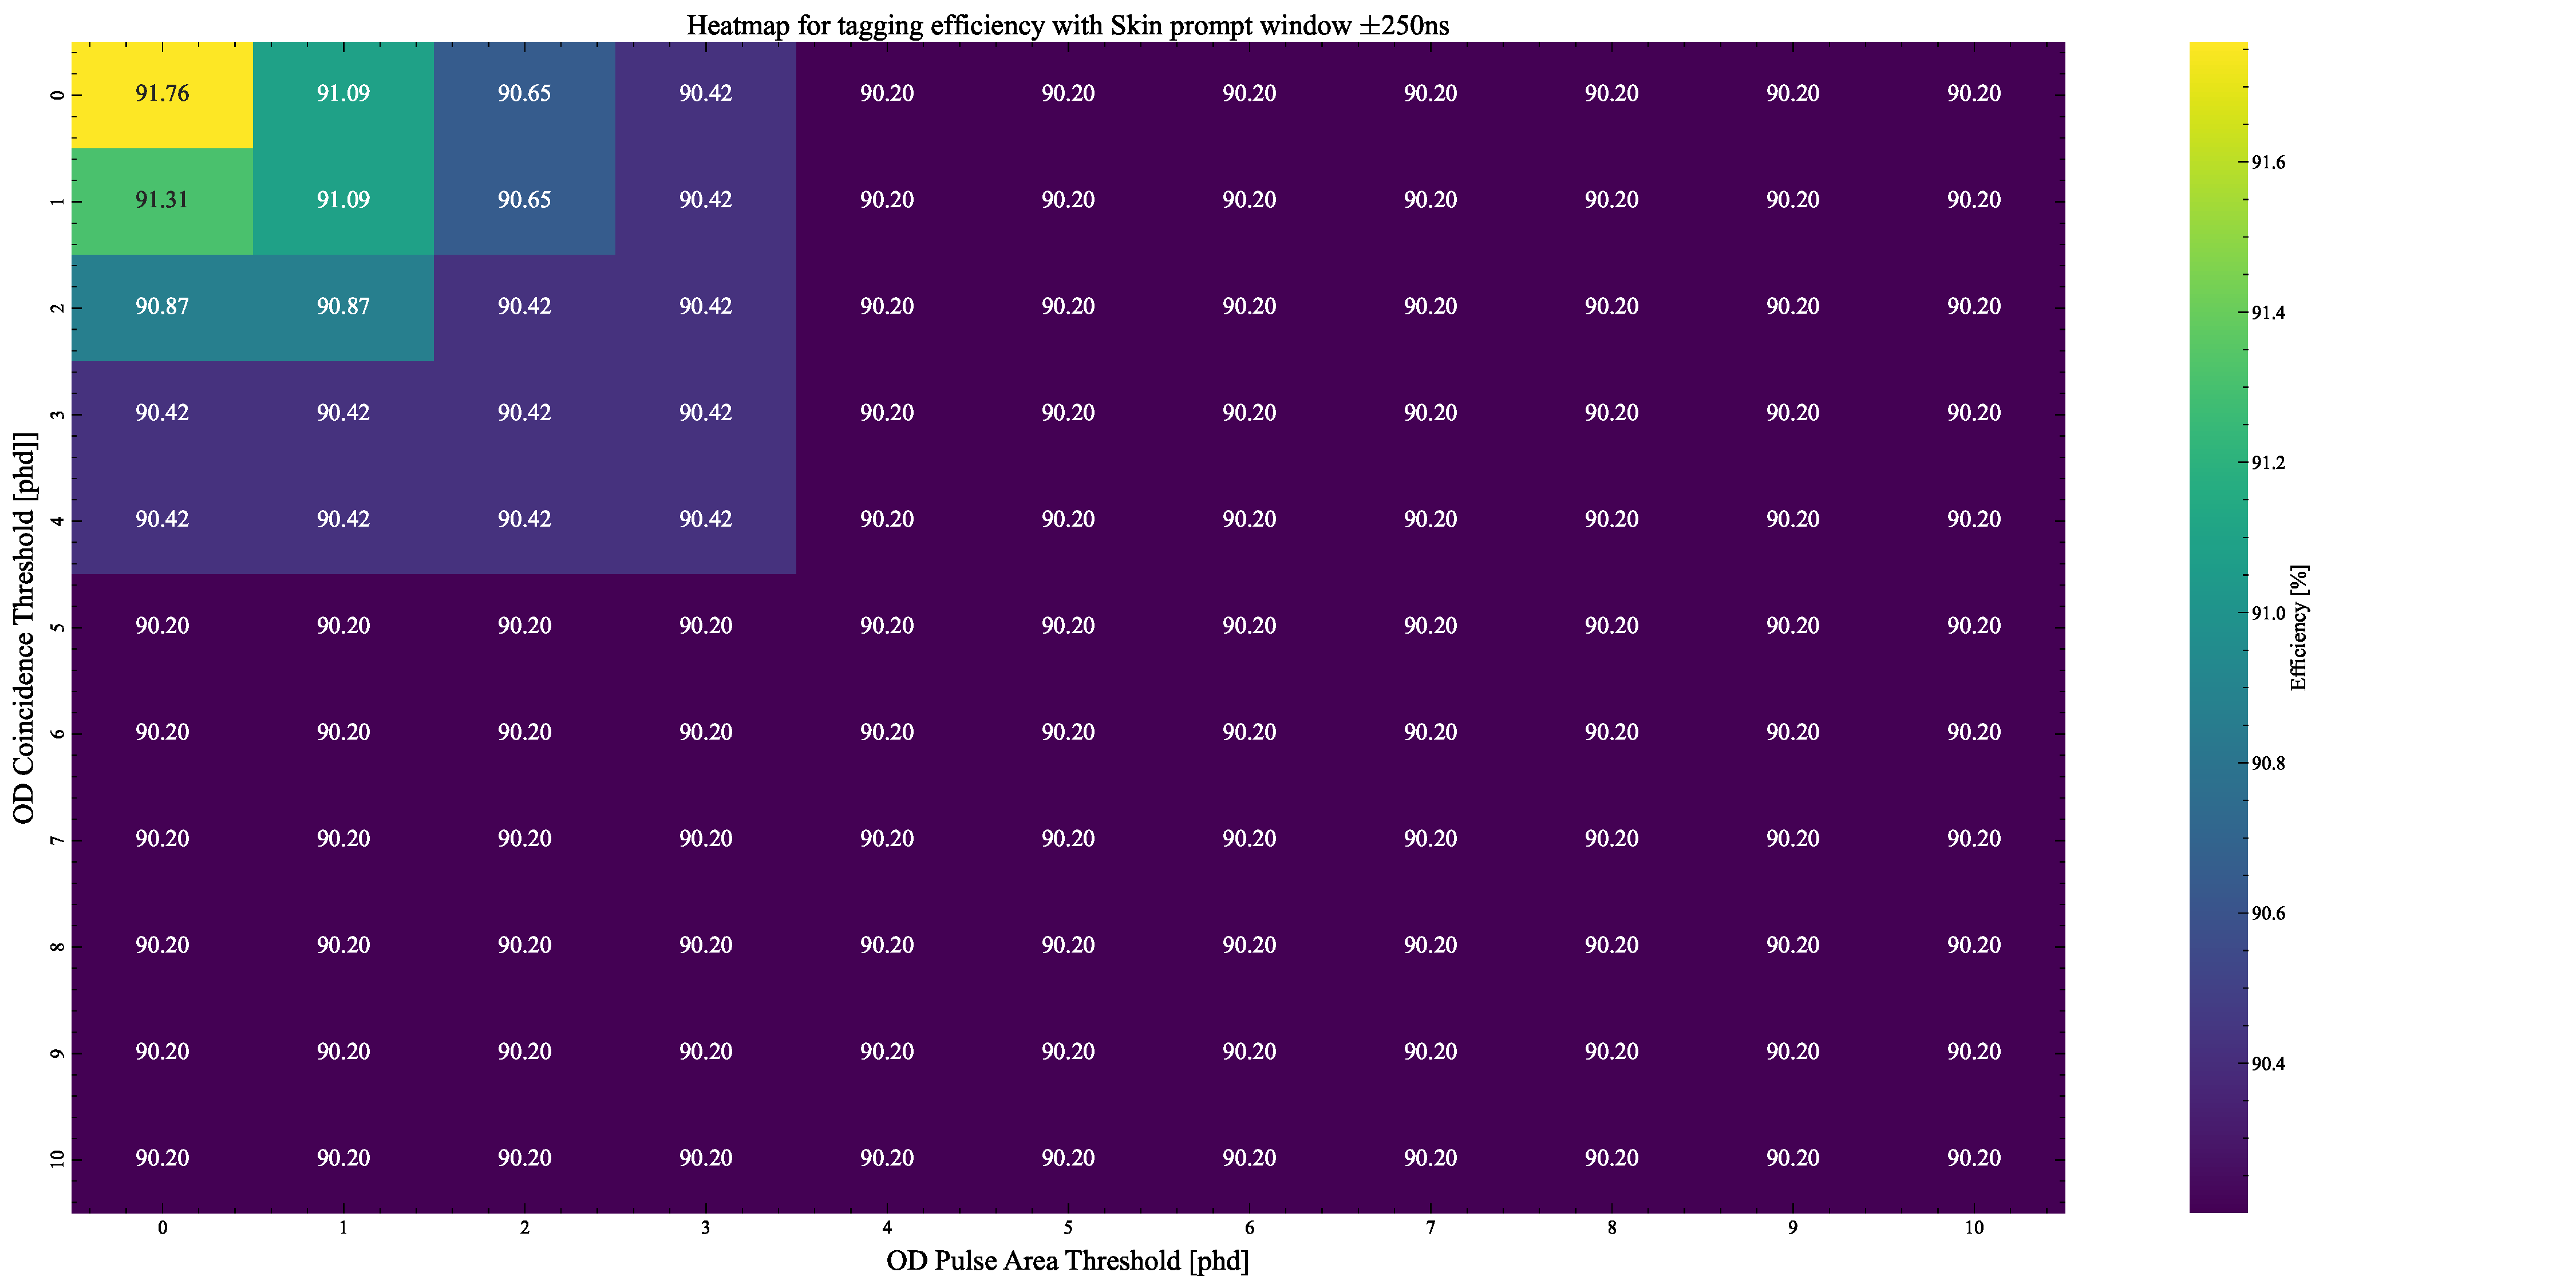
\includegraphics[width=\textwidth]{figures/VetoEfficiency/HeatmapSkinPACoinScanWindow500.pdf}
	\caption{Skin Prompt heatmap.
		In each bin, either the pulse coincidence or the pulse threshold has been varied.
		The z-axis shows the efficiency associated with a given pulse requirement.
		The veto time window considered is [-250, 250]ns.}
	\label{fig:VetoEff/skin_prompt_veto_heatmap}
\end{sidewaysfigure}
\begin{sidewaysfigure}
	\centering
	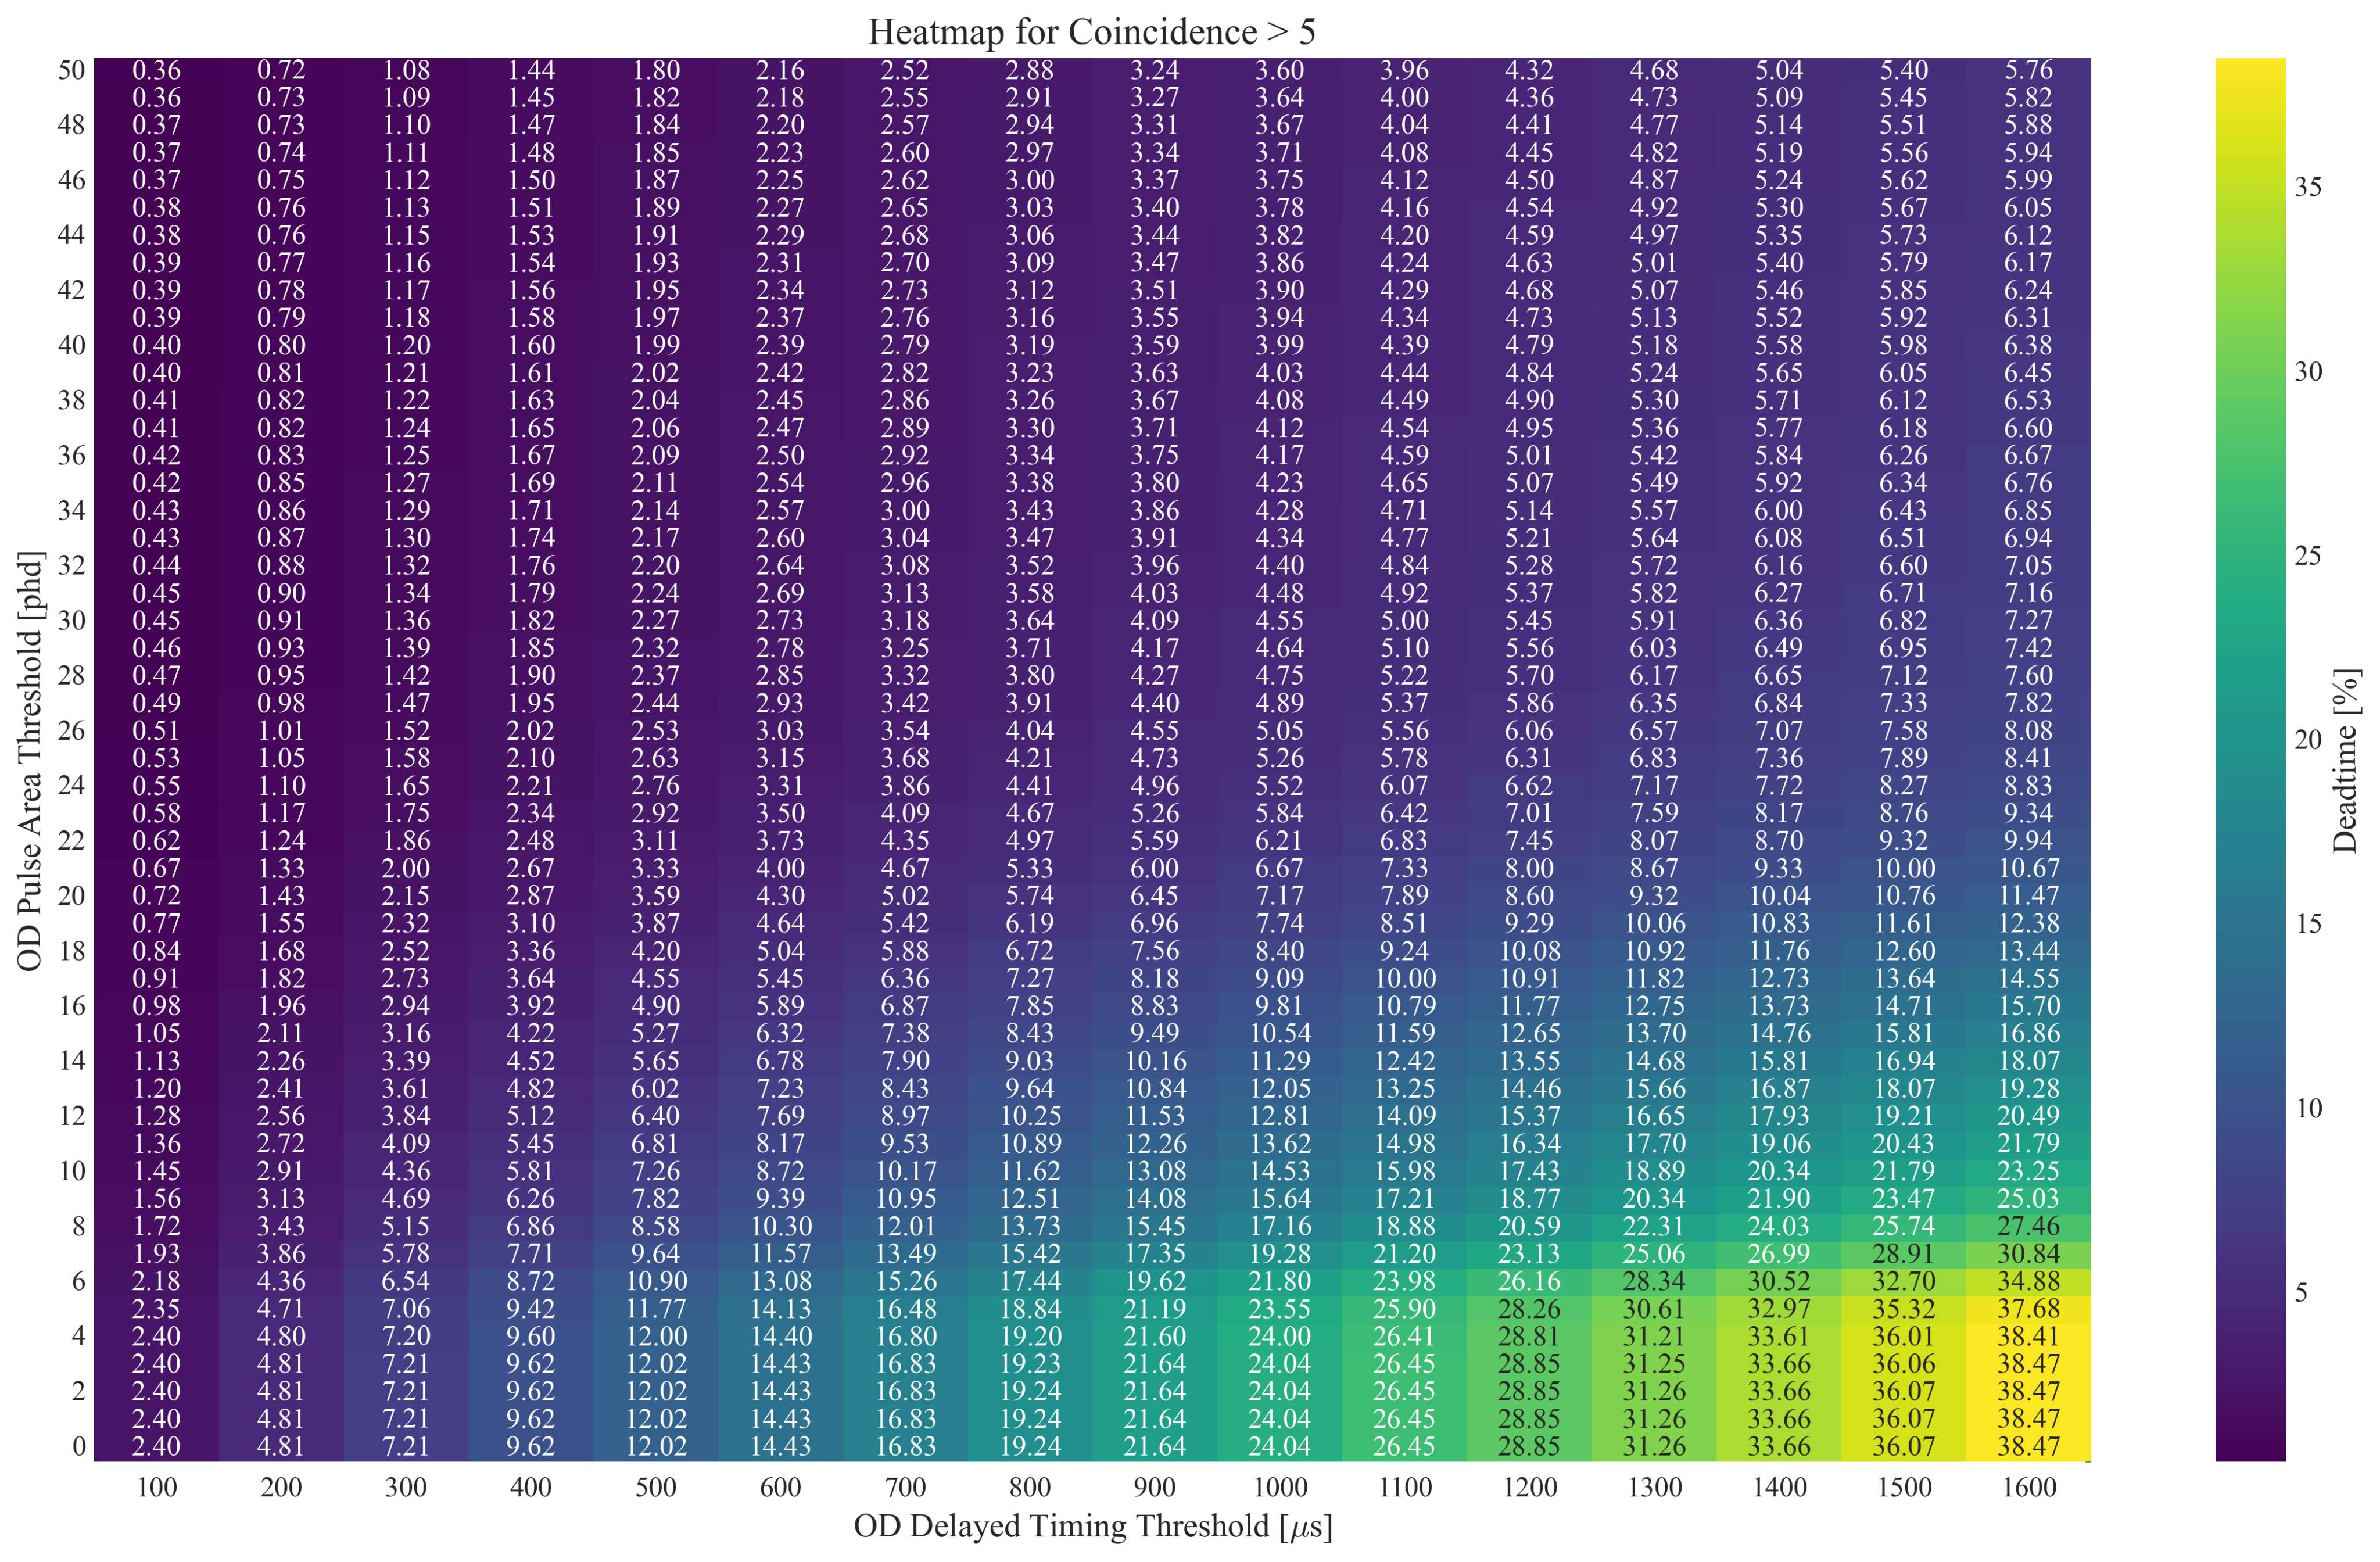
\includegraphics[width=\textwidth]{figures/VetoEfficiency/OD_Deadtime_thesis.png}
	\caption{OD Delayed heatmap.
		In each bin, either the veto window or the pulse threshold has been varied.
		The z-axis shows the deadtime associated with a given veto window and pulse threshold.
		In addition to the pulse area threshold, the pulse must have a coincidence greater than 5.}
	\label{fig:VetoEff/od_delayed_veto_heatmap}
\end{sidewaysfigure}
\begin{sidewaysfigure}
	\centering
	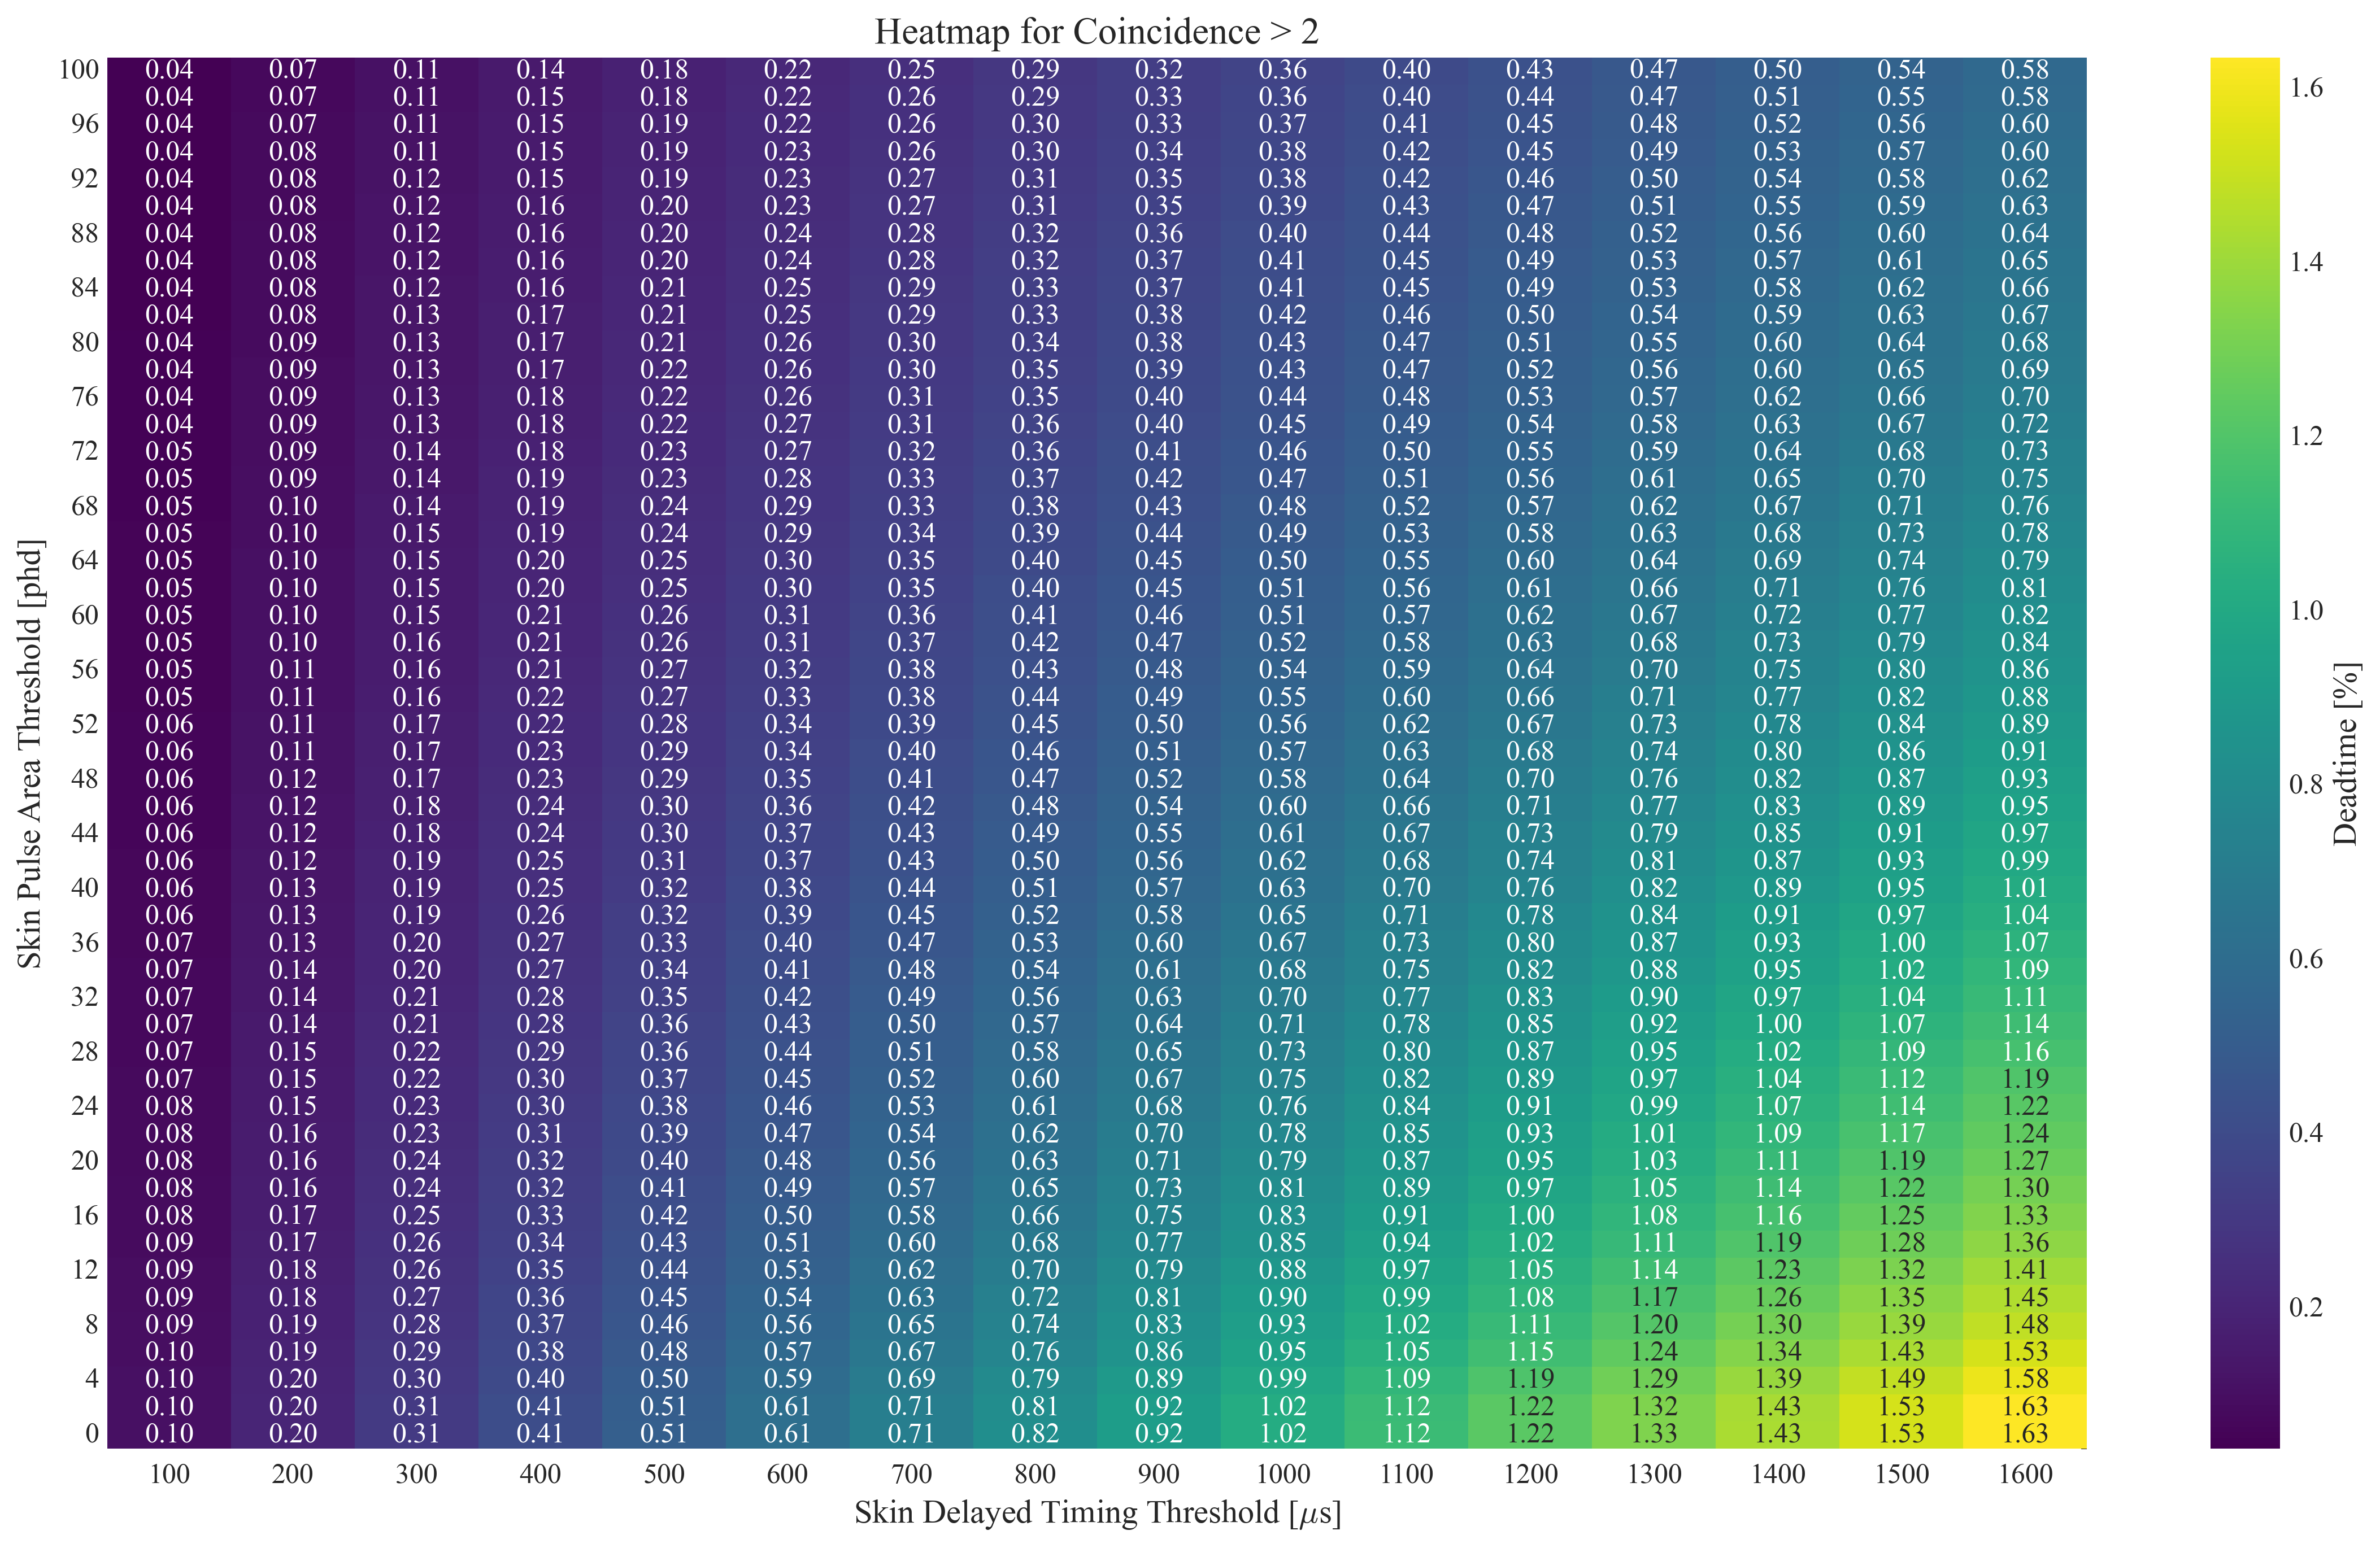
\includegraphics[width=\textwidth]{figures/VetoEfficiency/Skin_Deadtime_thesis.png}
	\caption{Delayed vetoes heatmap.
		In each bin, the OD pulse threshold or the Skin pulse threshold has been varied.
		The z-axis shows the veto efficiency associated with a given pulse thresholds.
		In addition to the pulse area threshold, the OD pulse must have a coincidence greater than 5, and the Skin pulse greater than 2.
		The veto window in this case is 500$\mu$s.}
	\label{fig:VetoEff/skin_delayed_veto_heatmap}
\end{sidewaysfigure}

\begin{figure}[!ht]
	\centering
	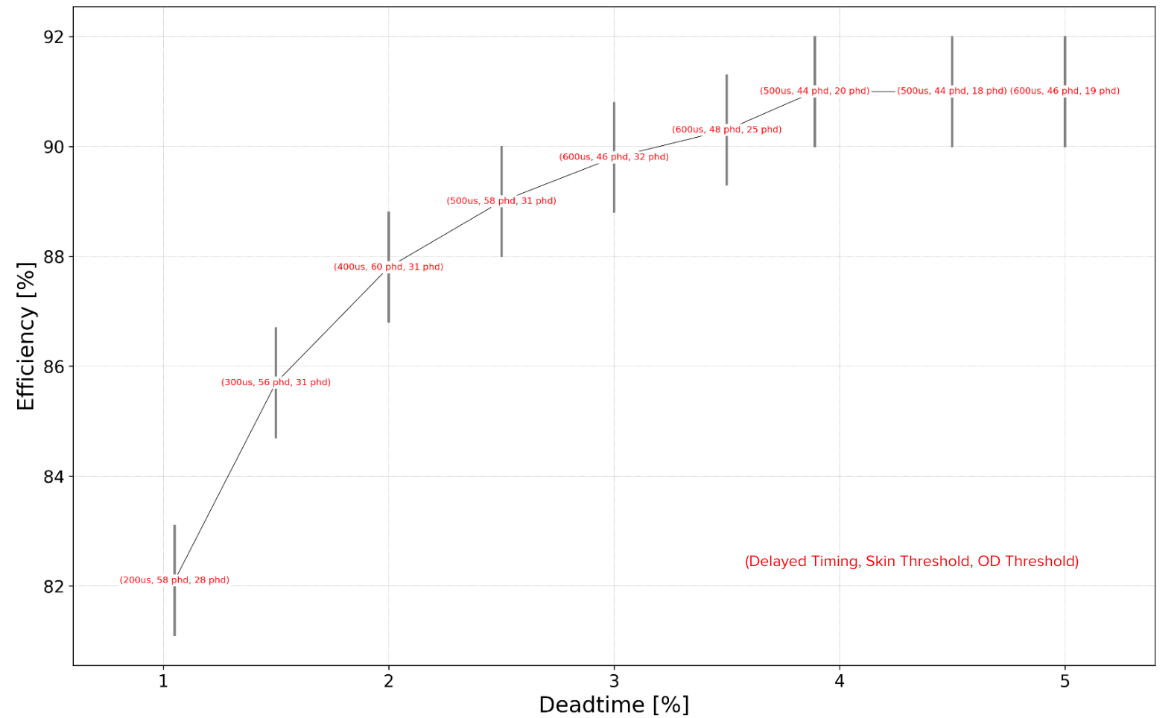
\includegraphics[width=0.9\textwidth]{figures/VetoEfficiency/cut_optimisation.png}
	\caption{Deadtime-vs-efficiency highlighting a number of considered cuts.
		At each point, the numbers in brackets are; the delayed veto window length after the TPC single-scatter, the Skin threshold pulse area, and the OD threshold pulse area.}
	\label{fig:VetoEff/veto_cut_optimisation}
\end{figure}

\iffalse
\begin{figure}[!ht]
	\centering
	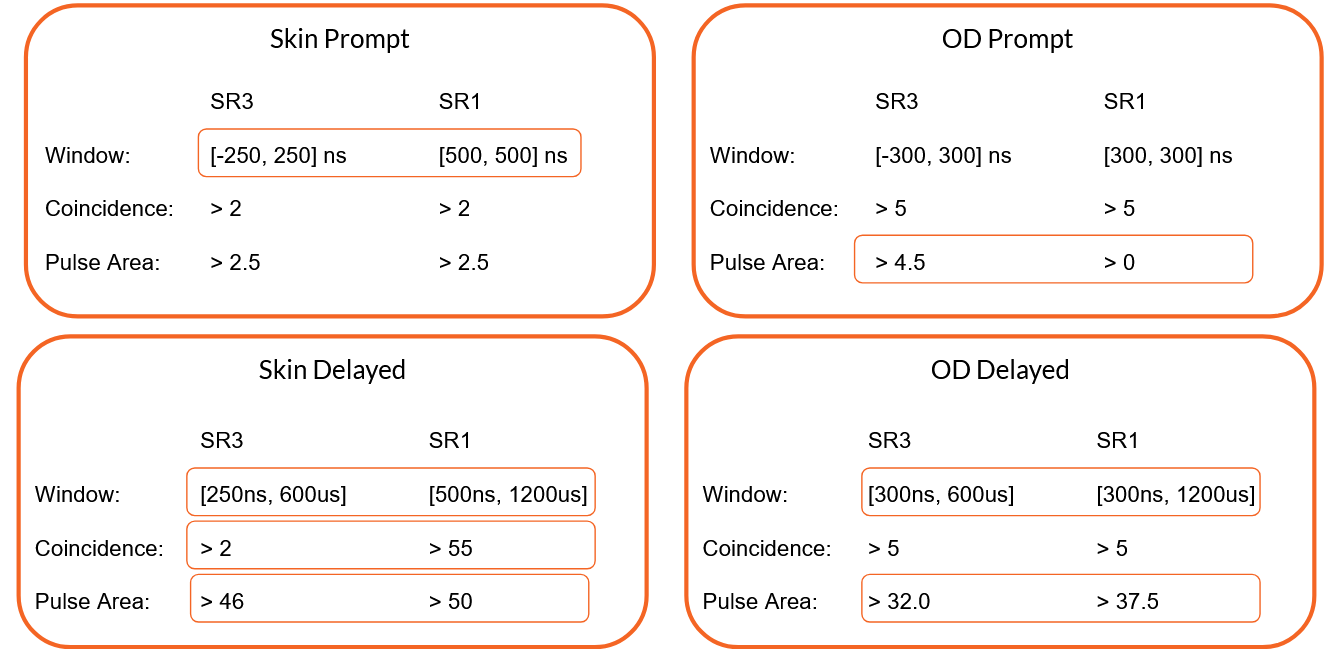
\includegraphics[width=0.9\textwidth]{figures/VetoEfficiency/sr3_cuts.png}
	\caption{Cuts determined to be optimal for the WS2024 science run.
		The WS2022 cuts are also included, where any modifications made to the selections is highlight accordingly.}
	\label{fig:VetoEff/sr3_veto_cuts}
\end{figure}
\fi

\begin{table}[!ht]
    \centering
    \caption{Cuts determined to be optimal for the WS2024 science run. The WS2022 cuts are also included, where any modifications made to the selections is highlighted accordingly. Coincidence corresponds to the number of PMTs which observe a pulse and pulse area is measured in `number of photons detected' [phd].}
    \scalebox{0.9}{
    \begin{tabular}{|c|c|c||c|c|c|}
    \hline
    \multicolumn{3}{|c||}{\textbf{Skin Prompt}} & \multicolumn{3}{c|}{\textbf{OD Prompt}} \\
    \hline
    & WS2024 & WS2022 & & WS2024 & WS2022 \\
    \hline
    Window & \cellcolor[HTML]{cecece} [-250,250]~ns & \cellcolor[HTML]{cecece}[500,500]~ns & Window & [-300,300]~ns & [-300,300]~ns\\
    Coincidence&$>2$&$>2$&Coincidence&$>5$&$>5$\\
    Pulse Area & $>2.5$ & $>2.5$ & Pulse Area & \cellcolor[HTML]{cecece}$>4.5$ &\cellcolor[HTML]{cecece} $>0$ \\    
    \hhline{|===||===|}
    \multicolumn{3}{|c||}{\textbf{Skin Delayed}} & \multicolumn{3}{c|}{\textbf{OD Delayed}} \\
    \hline
    &WS2024&WS2022&&WS2024&WS2022\\
    \hline
    Window&\cellcolor[HTML]{cecece}[250~ns, 600~$\mu$s]&\cellcolor[HTML]{cecece}[500~ns, 1200~$\mu$s]&Window&\cellcolor[HTML]{cecece}[300~ns, 600~$\mu$s]&\cellcolor[HTML]{cecece}[300~ns, 1200~$\mu$s]\\
    Coincidence&\cellcolor[HTML]{cecece}$>2$&\cellcolor[HTML]{cecece}$>55$&Coincidence&$>5$&$>5$\\
    Pulse Area&\cellcolor[HTML]{cecece}$>46$&\cellcolor[HTML]{cecece}$>50$&Pulse Area&\cellcolor[HTML]{cecece}$>32.0$&\cellcolor[HTML]{cecece}$>37.5$\\
    \hline
    \end{tabular}}
    \label{tab:VetoEff/sr3_veto_cuts}
\end{table}

\subsection{Deadtime stability}\label{sec:VetoEff/DeadtimeStability}
The deadtime for each of the veto cuts was checked for stability over the WS2024 science run.
%This was done by breaking up the WS2024 file list, in this case, \textbf{SR3-WSv7-LZAP-5.8.0}, into month-by-month chunks.
This was done by breaking up the WS2024 file list into month-by-month chunks.
For each month, the rate of pulses in the Skin and OD from the second half of Random Trigger data was used; and the rate above threshold where the threshold is based on the particular veto cut is recorded. 
The stability of this over WS2024 is shown in \autoref{fig:VetoEff/deadtime_stability}.
The deadtime is then calculated as;
\begin{equation}
	\textrm{Dead Time [\%]} = 1 - e^{-\lambda (x)}
\end{equation}
where $\lambda$ is the background rate and $x$, the veto threshold.
%The deadtime can also be approximated by;
%\begin{equation}
%    \textrm{Approx. Dead Time [\%]} = \textrm{Rate of events above threshold [Hz]} \times \textrm{Veto window length [s]} \times 100
%\end{equation}

The conclusion that the deadtime is stable over WS2024 was additional checked by looking at the \lstinline{ODHealth} PREM module, shown in \autoref{fig:VetoEff/deadtime_stability_prem}.
The PREM module shows the rate of OD pulses above $200~\text{keV}$ (as defined by the WS2022-$200~\text{keV}$ not from the WS2024 energy calibration), with no significant fluctuation during WS2024.
\begin{figure}[!ht]
	\centering
	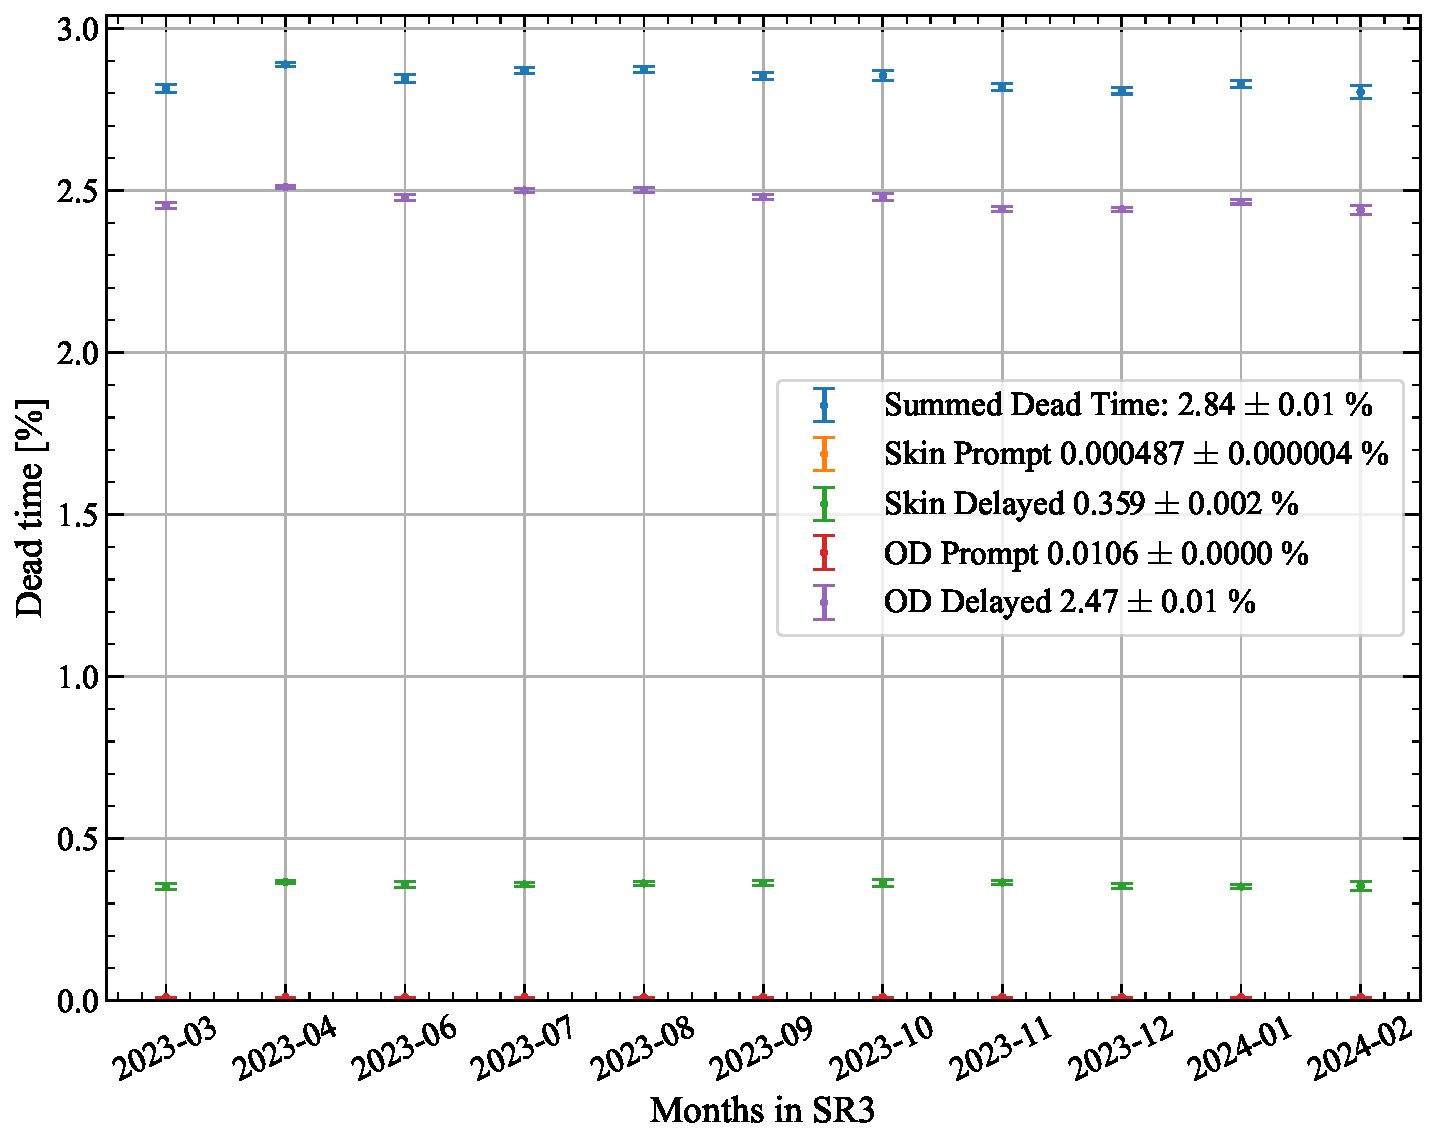
\includegraphics[width=0.8\textwidth]{figures/VetoEfficiency/SR3DeadTimeAll_expoFunc.pdf}
	\caption{Deadtime from the Skin and OD veto cuts during each month of WS2024 science run. The error shown in purely statistical.}
	\label{fig:VetoEff/deadtime_stability}
\end{figure}
\begin{figure}[!ht]
	\centering
	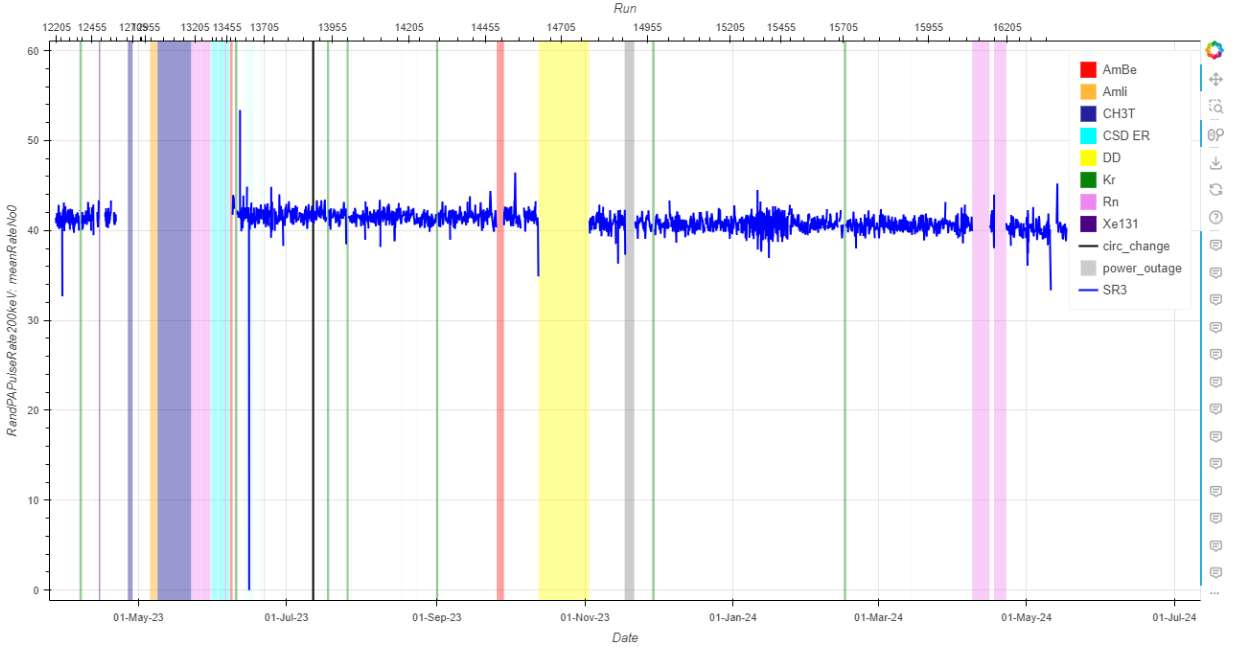
\includegraphics[width=\textwidth]{figures/VetoEfficiency/prem_od_stability.png}
	\caption{Rate of OD pulses above 200~keV (as defined by WS2022 energy calibration) over the WS2024 science run. Various periods of calibration are indicated by the coloured regions.}
	\label{fig:VetoEff/deadtime_stability_prem}
\end{figure}

\section{Neutron veto efficiency}\label{sec:VetoEff/efficiency}
In this section, the efficiency of tagging background neutrons using the Skin and OD detectors is calculated.
This is performed by calculating the efficiency on AmLi and DD calibration data.
This is then compared to AmLi and DD simulations.
The difference between these simulations and data are then used to calculate an offset.
The efficiency is then calculated for detector NR simulations and the offset applied (either a subtraction or a scaling, discussed later).
This gives the neutron tagging efficiency for background neutrons.
\subsection{Efficiency calculation}
The efficiency is defined as;
\begin{equation}
	\epsilon [\%] = \frac{\textrm{N. Events passing Analysis Cuts + Veto Cuts}}{\textrm{N. Events passing Analysis Cuts}} \times 100
	\label{eqn:VetoEff/:neutron_tagging_efficiency}
\end{equation}
and the inefficiency is defined as $100 - \epsilon$.

\subsection{Neutrons from calibration sources \label{sec:VetoEff/AmLi_Efficiency}}
\subsubsection{AmLi}
The AmLi calibration runs are from the May 2023 calibration period before the WS2024 science run, with run control operation name \textbf{Amli-B}.
The runs used were; \lstinline{13004-13026}.
All files were processed with \lstinline{LZAP-5.8.0}.

On these events, the selection of cuts were applied.
The majority of which are `standard' WS2024 Core Cuts which are listed in \autoref{tab:VetoEff/amli_efficiency_cuts}.
In addition to the cuts listed in \autoref{tab:VetoEff/amli_efficiency_cuts}, two other categorizes of cuts were applied:
\begin{enumerate}
	\item \textbf{CSD tube}: This is a circular cut on the reconstructed position of the SS in the TPC so that events from just one CSD tube are selected at a time.
	To make the comparison between data and simulation this cut is required because in simulation only one source in one tube was simulated as opposed to deploying a source in each CSD tube simultaneously.
	This is useful for examining the fluctuation in neutron tagging efficiency with $(x,y,z)$.
	When the efficiency is averaged across different heights and CSD tube, the average can then be replicated in both data and simulation. The cut uses the following logic;  
\begin{lstlisting}[backgroundcolor=\color{lightgray},language=Python]
def CSDSelection(x: float, y: float, which_csd: int=1):
    cent_csd_x = [87.6, -43.9, -43.9]
    cent_csd_y = [-0.13, 75.7, -75.7]
    x_el = pow((x-cent_csd_x[which_csd]),2)
    y_el = pow((y-cent_csd_y[which_csd]),2)
    r2_el = x_el + y_el
    return r2_el < 50**2
\end{lstlisting}
	      How this looks in $(x,y)$ is shown in \autoref{fig:VetoEff/CSDSelection}.
	      A concern of this cut is that events towards the centre of the TPC are excluded.
	      However, the position averaged efficiency when the CSD cut and not is $(88.21\pm1.03)\%$ and  $(88.25\pm1.22)\%$ respectively.
	      Across the $600\mu s$ window, there is no greater than $2\%$ difference between when the cut is and isn't applied.
	      This comparison can be seen in \autoref{fig:VetoEff/CSDSelectionEffComp}.
	\item \textbf{NR-band}: This is a 1-, 3-, or 5-$\sigma$ cut around the NR band median.
	      The purpose of this cut is to improve the purity of the selection.
	      In this analysis, the 1-$\sigma$ was used.
	      %The band can be found on NERSC at \lstinline{/global/cfs/cdirs/lz/physics/NEST_Bands/SR3/20240313/Calibration}, if the band has been, it can be recreated with the Woods parameters listed below;
		  The band was generated using the Noble Element Simulation Technique (NEST), it can be recreated with the Woods parameters listed below;
\begin{lstlisting}[backgroundcolor = \color{lightgray}]
The Woods Function Fit Parameters for the Band Mean are:
[-6.709932875296116, 7.230400677496497,
0.001868430053684265, 3.648854814073587]

The Woods Function Fit Parameters for the -1 Sigma Line are:
[-7.995805026708432, 7.163090296730374,
0.0018689902999408099, 3.6135843431273336]

The Woods Function Fit Parameters for the +1 Sigma Line are:
[-5.428217339686645, 7.337771458785042,
0.0018671903851709354, 3.684225777881352]
\end{lstlisting}
The three different NR bands for the three calibration sources can be seen in \autoref{fig:VetoEff/SR3NRBands}.
\end{enumerate}

\begin{figure}[!ht]
	\centering
	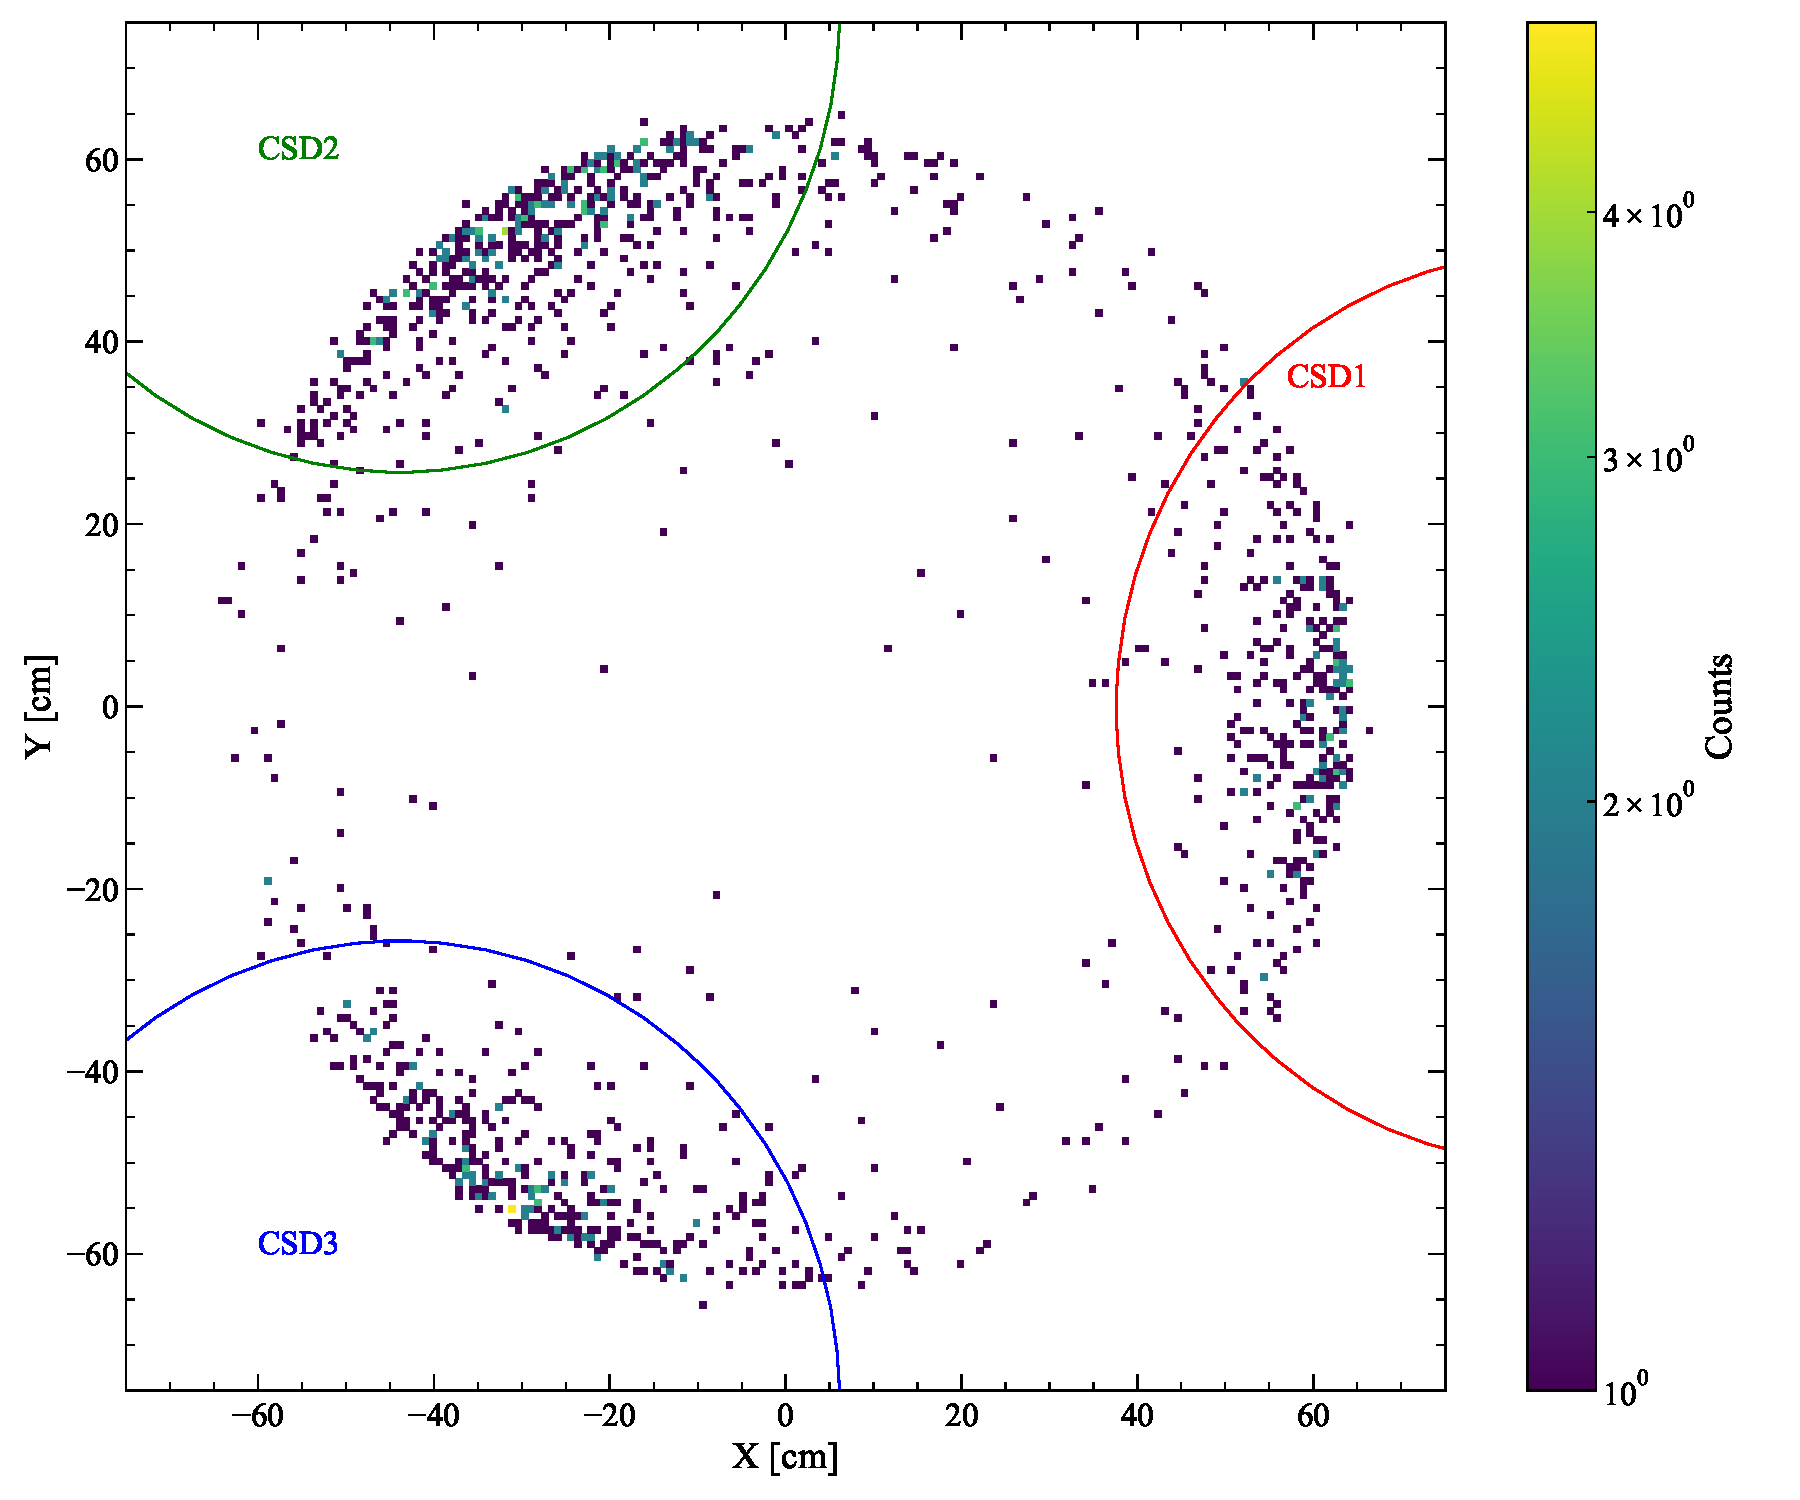
\includegraphics[width=0.8\textwidth]{figures/VetoEfficiency/CircularCSDCut.pdf}
	\caption{X-Y distribution of events in the TPC for AmLi sources positioned at 700mm. Each of the circular cuts are overlaid onto the plot.}
	\label{fig:VetoEff/CSDSelection}
\end{figure}
\begin{figure}[!ht]
	\centering
	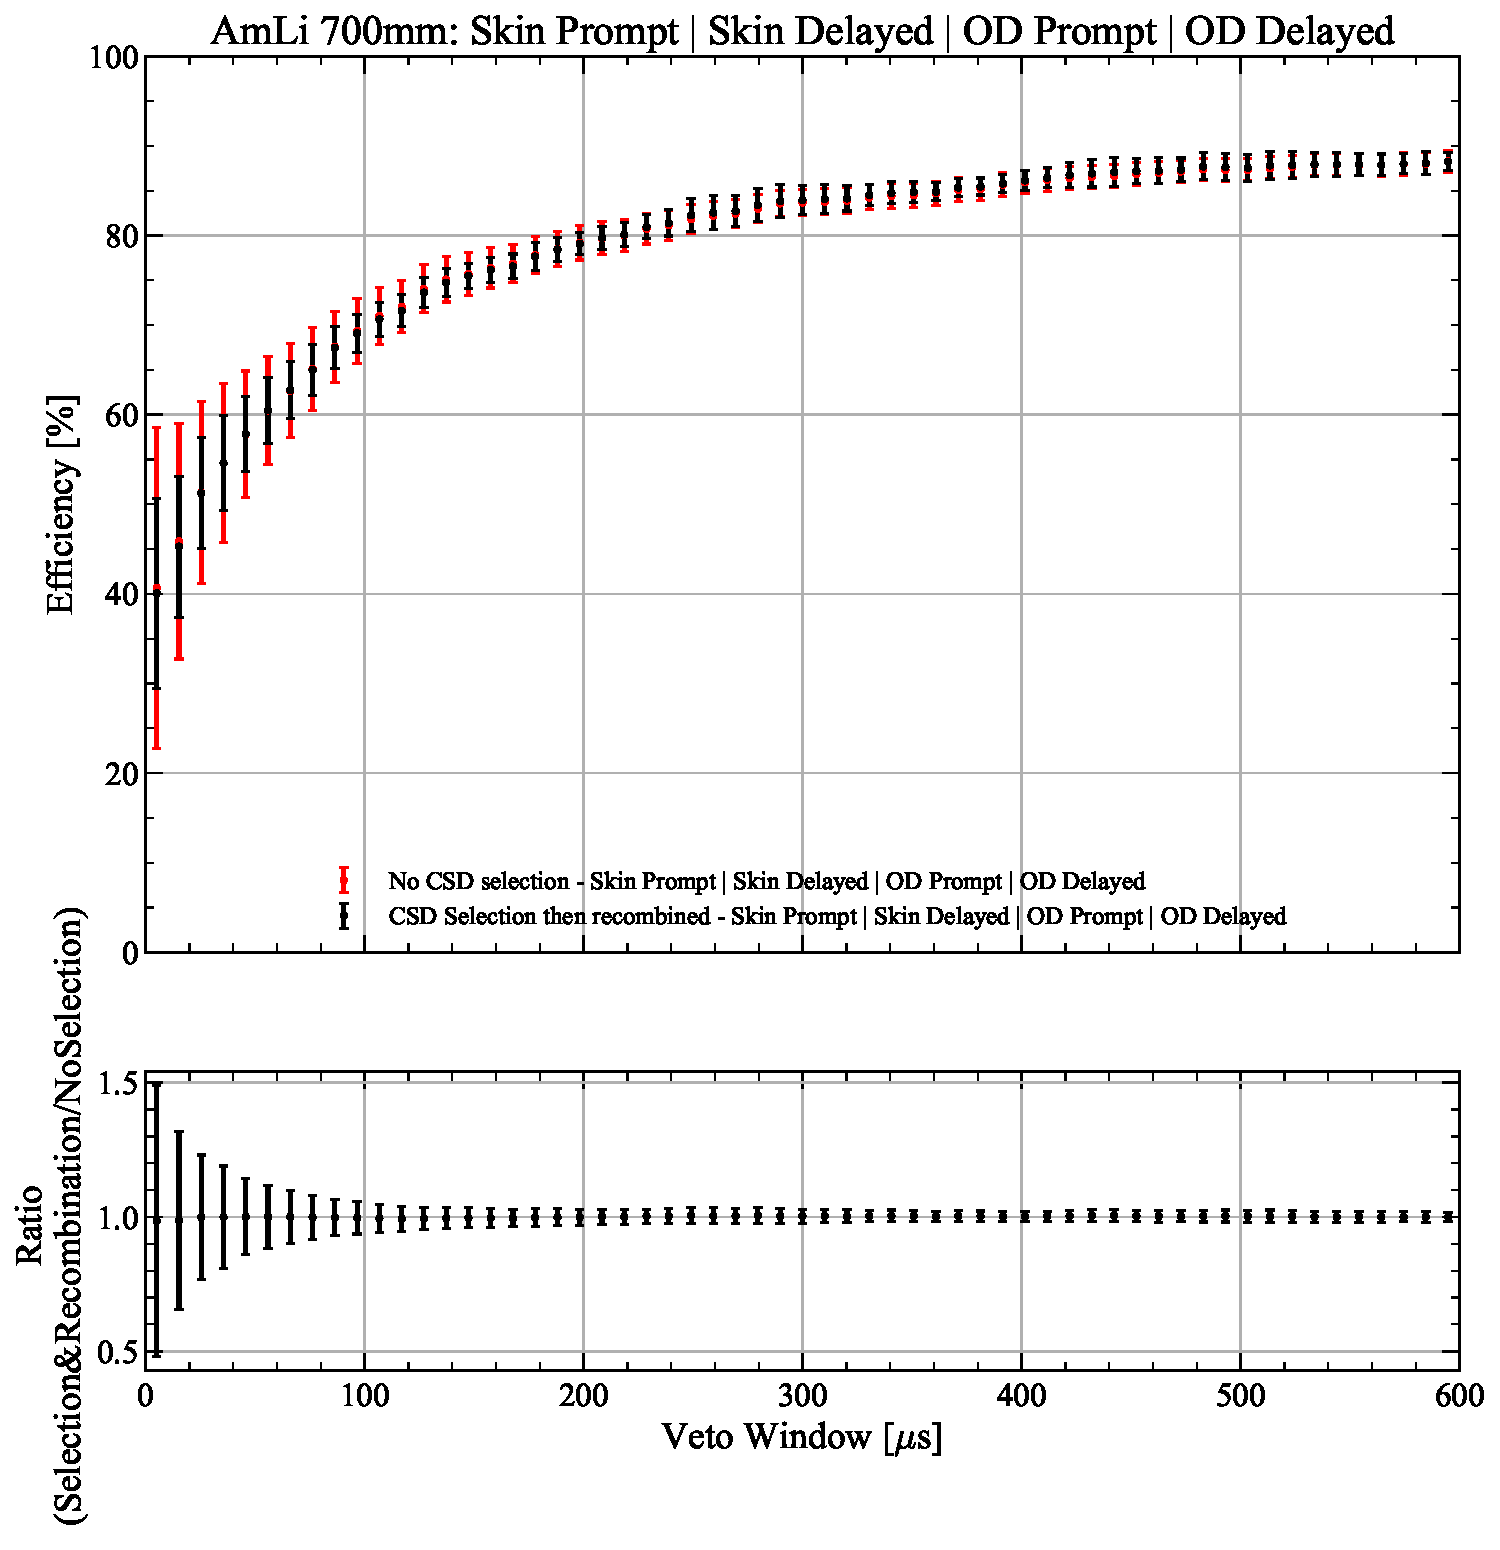
\includegraphics[width=0.8\linewidth]{figures/VetoEfficiency/AmLi_700mm_Total_CSDSelection.pdf}
	\caption{The veto efficiency (from all analysis cuts) at using AmLi at 700mm. The ratio plot shows the less than $2\%$ difference between method 1 and method 2.}
	\label{fig:VetoEff/CSDSelectionEffComp}
\end{figure}
\begin{figure}[!ht]
	\centering
	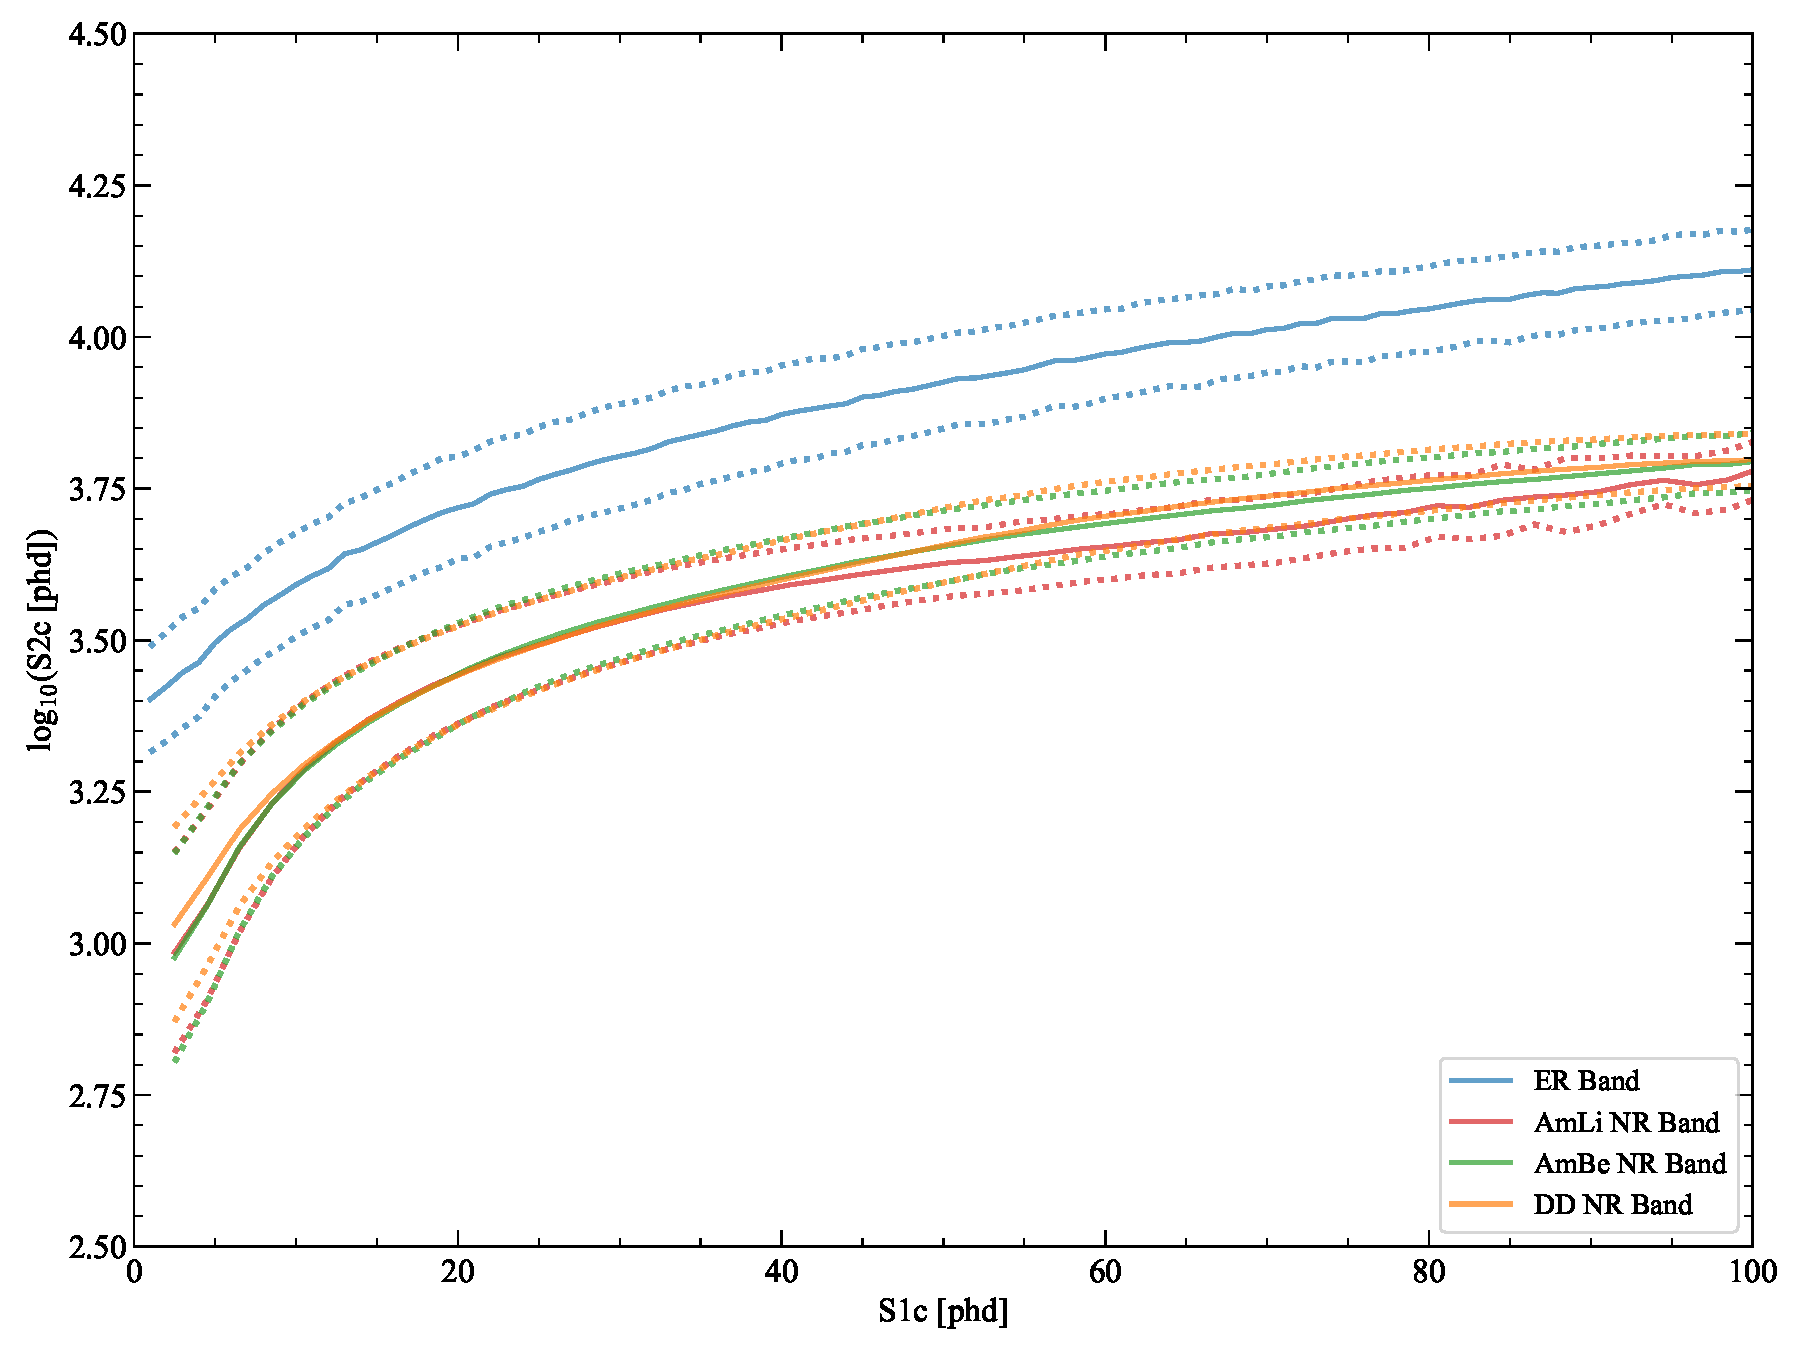
\includegraphics[width=0.8\textwidth]{figures/VetoEfficiency/SR3NRBands.pdf}
	\caption{The three different NR bands used for the NR-band cut for the respective sources, AmLi, DD. NEED TO REMOVE AmBe BAND HERE.}
	\label{fig:VetoEff/SR3NRBands}
\end{figure}
\begin{table}[!ht]
	\centering
    \scalebox{0.9}{
	\caption{ALPACA-Core WS2024 cuts used on AmLi calibration data for determining the efficiency.}
	\begin{tabular}{|c|c|c|c|}
    \hline
    \textbf{Livetime cuts}&\textbf{ Physics cuts}& \textbf{S1 cuts}& \textbf{S2 cuts}\\
    \hline
    Burst noise cut& Single scatter& S2 width vs drift time& S1 prominence cut\\
    Muon holdoff& S1 and S2 threshold & Narrow S2& Stinger event cut\\
    Sustained rate cut& Fiducial Volume& S2 rise time& S1 TBA vs drift time \\
    High S1 rate exclusion & & S2 early peak& S1 HSC cut\\
    Bad buffer cuts& & S2 XY quality& S1 shape\\
    Excess Area cut& & S2 TBA & S1 photon timing\\
    \hline
	\end{tabular}}
	\label{tab:VetoEff/amli_efficiency_cuts}
\end{table}

\subsubsection{AmLi accidental correction}\label{sec:VetoEff/AmLiAccCorrection}
When determining the veto tagging efficiency a correction must be applied to the measured efficiency to account for the accidental coincidences from AmLi gammas (and neutrons) with single scatter nuclear recoils in the TPC which can artificially enhance the measured tagging efficiency.
First, veto inefficiency must be defined. Every time a single scatter nuclear recoil is observed in the TPC, a veto window is opened, this can be recorded using a counter, $N$ every time this happens.
If there is no pulse observed in the Skin or the OD that satisfies the veto requirements, this event is not vetoed and recorded using a counter, $M$. Resulting in a total inefficiency, $M/N$, and a total efficiency, $1-M/N$.
The effect of the accidentals be a result of the following process.
If a neutron enters the TPC, scatters and is not detected by the vetos, the counter $M$ should be iterated but there is an accidental coincidence of a gamma or a neutron from the AmLi sources with the TPC scatter so the count is not iterated.
The probability of this happening can be written as $1-P_a(0)$, where $P_a(0)$ is the probability of seeing zero accidental pulses in the Skin and OD coincidence windows.
Using probability and the counters, the true inefficiency is described below,
\begin{gather*}
	M_{observed}=M_{true}-M_{true}(1-P_a(0)) \\
	M_{observed}=M_{true}P_a(0)\rightarrow M_{true}=M_{observed}/P_a(0)\\
	Ineff_{true}=M_{true}/N\;and\;Ineff_{observed}=M_{observed}/N\\
	\Rightarrow Ineff_{true}=Ineff_{observed}/P_a(0)
\end{gather*}
Due to the logic of the inefficiency calculation is that the $M$ counter iterates in an AND condition such that all coincidence windows in all detector have to be empty.
This leads to a final inefficiency of,
\begin{equation}
	Ineff_{true} = Ineff_{obs}  / (1 - P_a(>0)_{any\:window})
\end{equation}
$P_a(>0)_{any\:window}$ can be determined directly using the post-trigger window of randomly triggered events (GPS events) and count any pulses in \textbf{any} of the veto detectors.
The accidental correction is correlated with the length of the veto window, scans over the entire delayed veto window in 10$\mu$s steps, the change in the correction factor over time can be seen in \autoref{fig:VetoEff/AccCorr}.
The impact of the accidental correction when applied to the efficiency can be seen in \autoref{fig:VetoEff/AccidentalImpact}.
\begin{figure}[!ht]
	\centering
	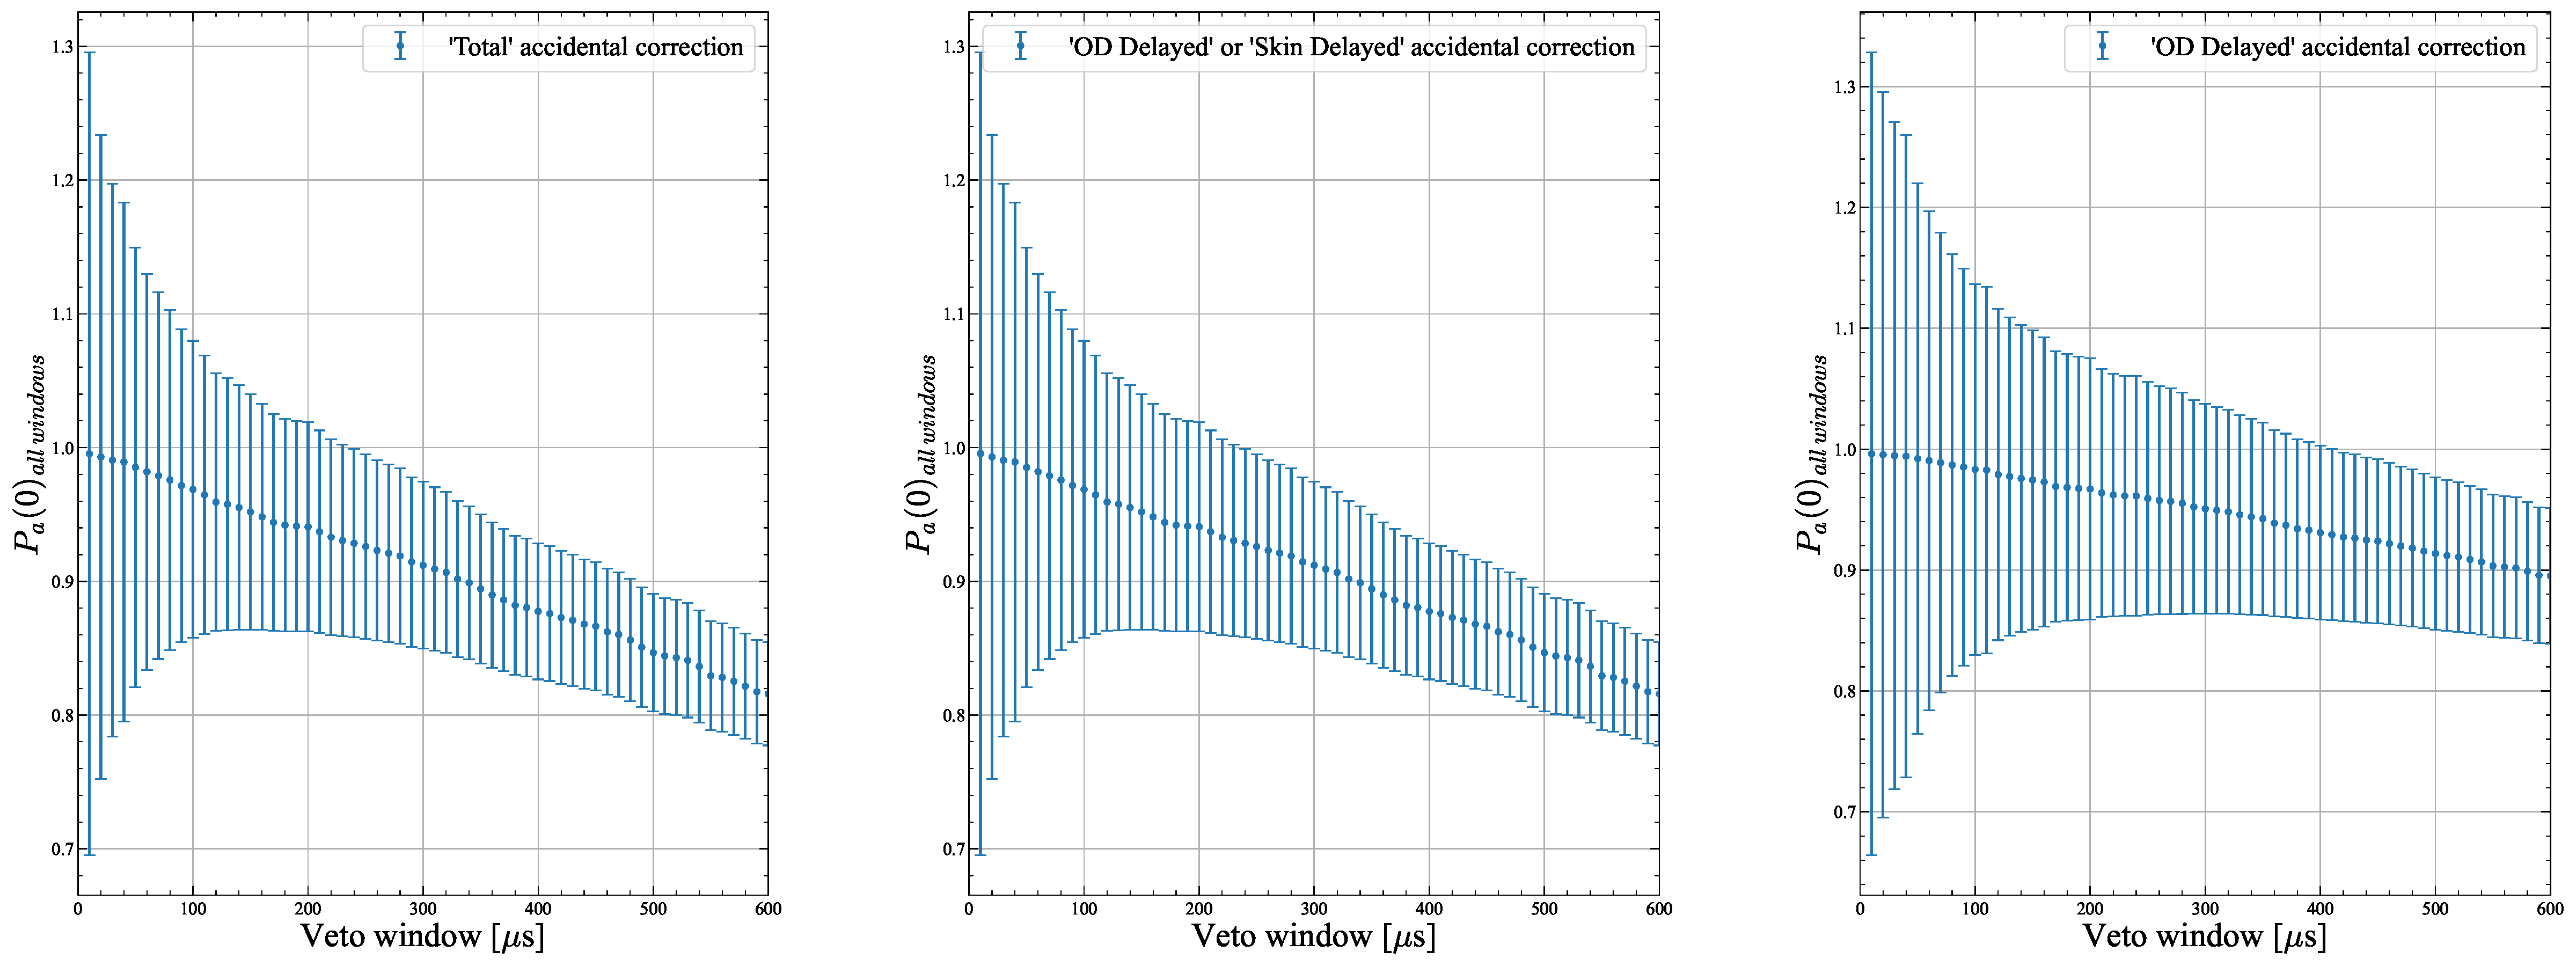
\includegraphics[width=\textwidth]{figures/VetoEfficiency/SR3AmLi_700_Corrections_100k_P0.pdf}
	\caption{$P_a(>0)_{all\:window}$ AmLi Accidental correction factors for varying veto window size for different windows of interest.}
	\label{fig:VetoEff/AccCorr}
\end{figure}
\begin{figure}[!ht]
	\centering
	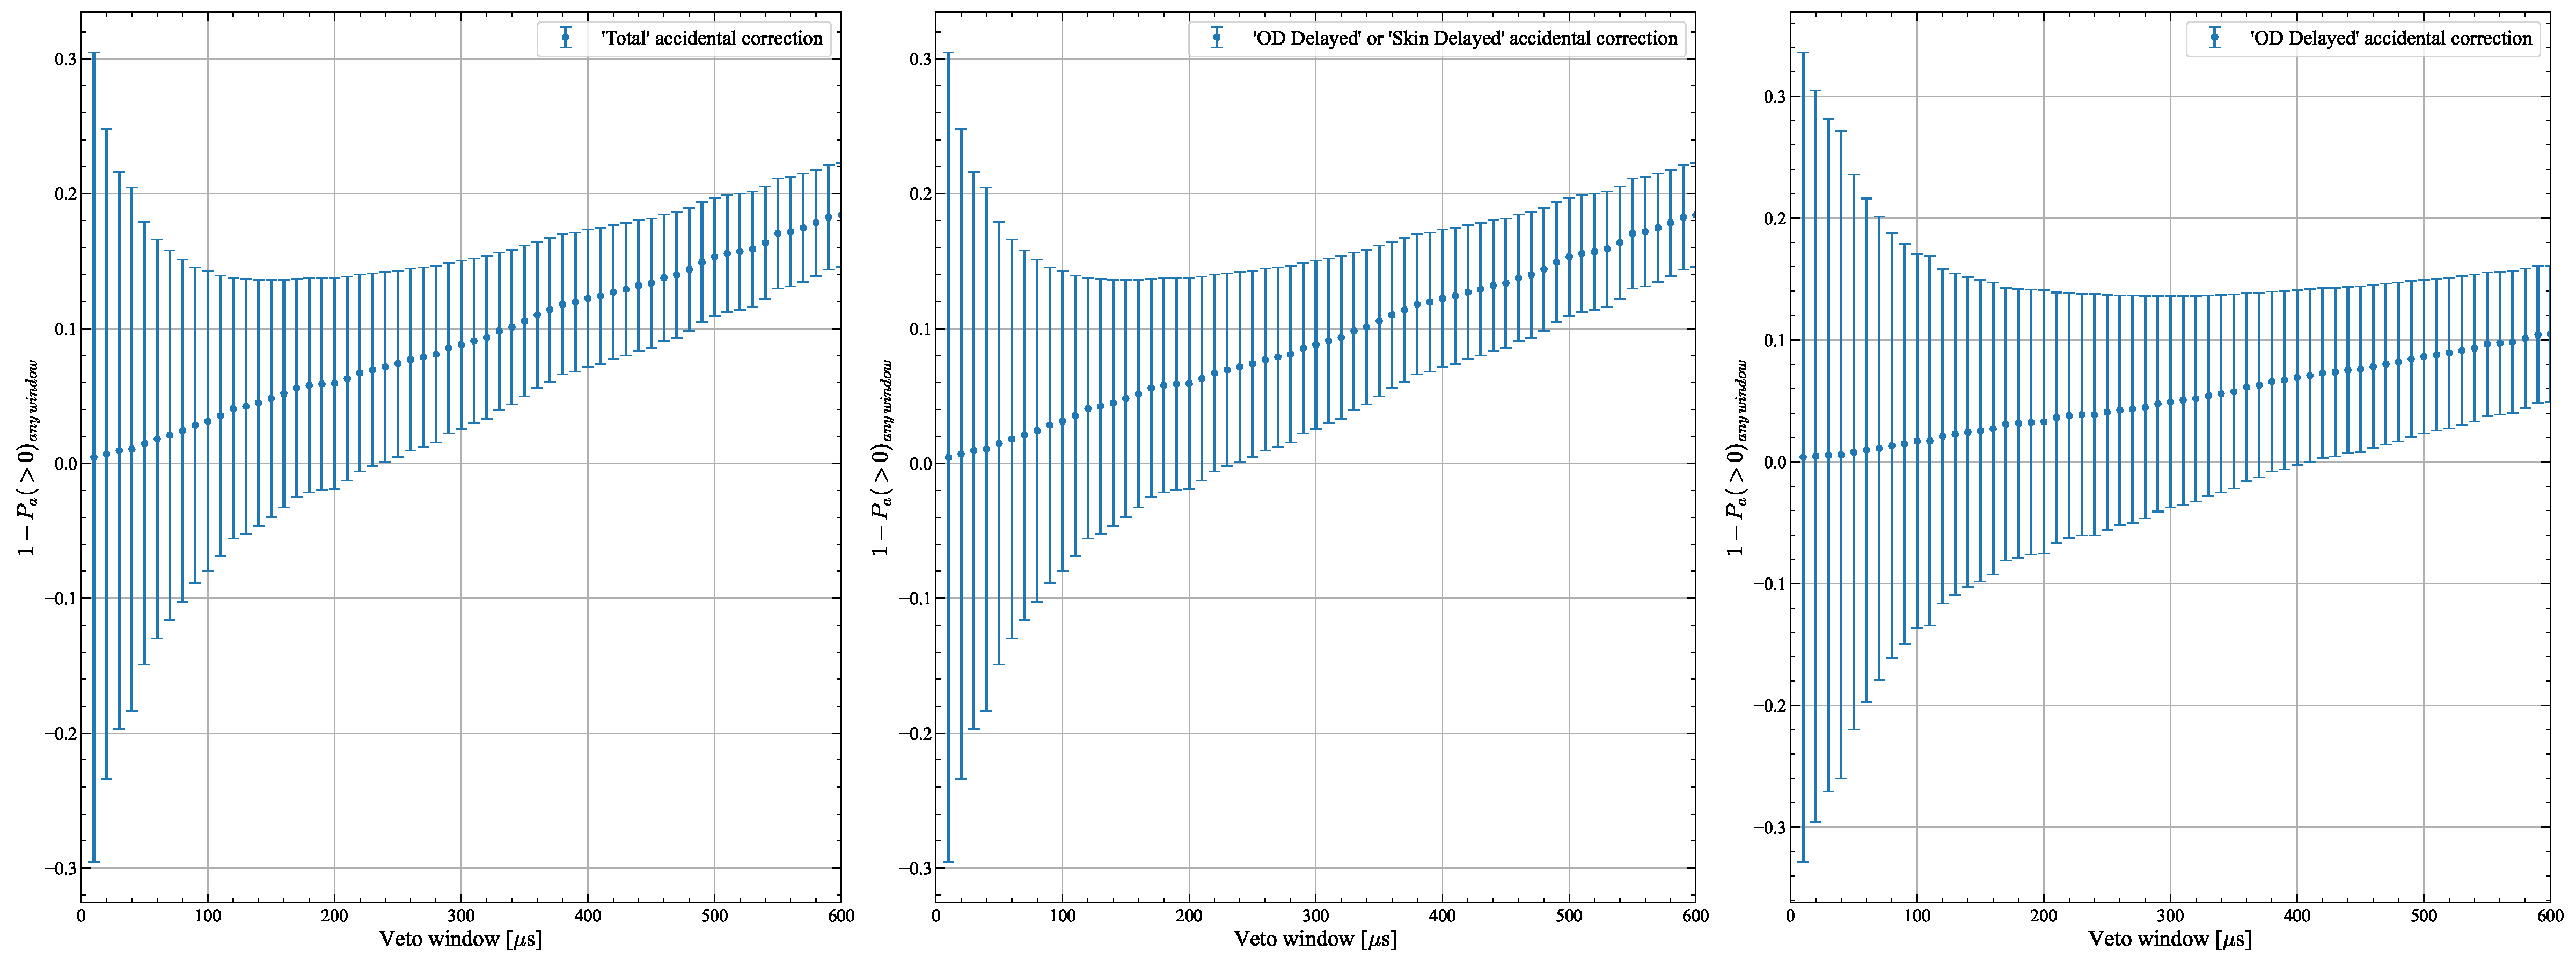
\includegraphics[width=\textwidth]{figures/VetoEfficiency/SR3AmLi_700_Corrections_100k_P0-1.pdf}
	\caption{$1 - P_a(>0)_{any window}$ AmLi Accidental correction factors for varying veto window size for different windows of interest.}
	\label{fig:VetoEff/AccCorr_P0-1}
\end{figure}
\begin{figure}[!ht]
	\centering
	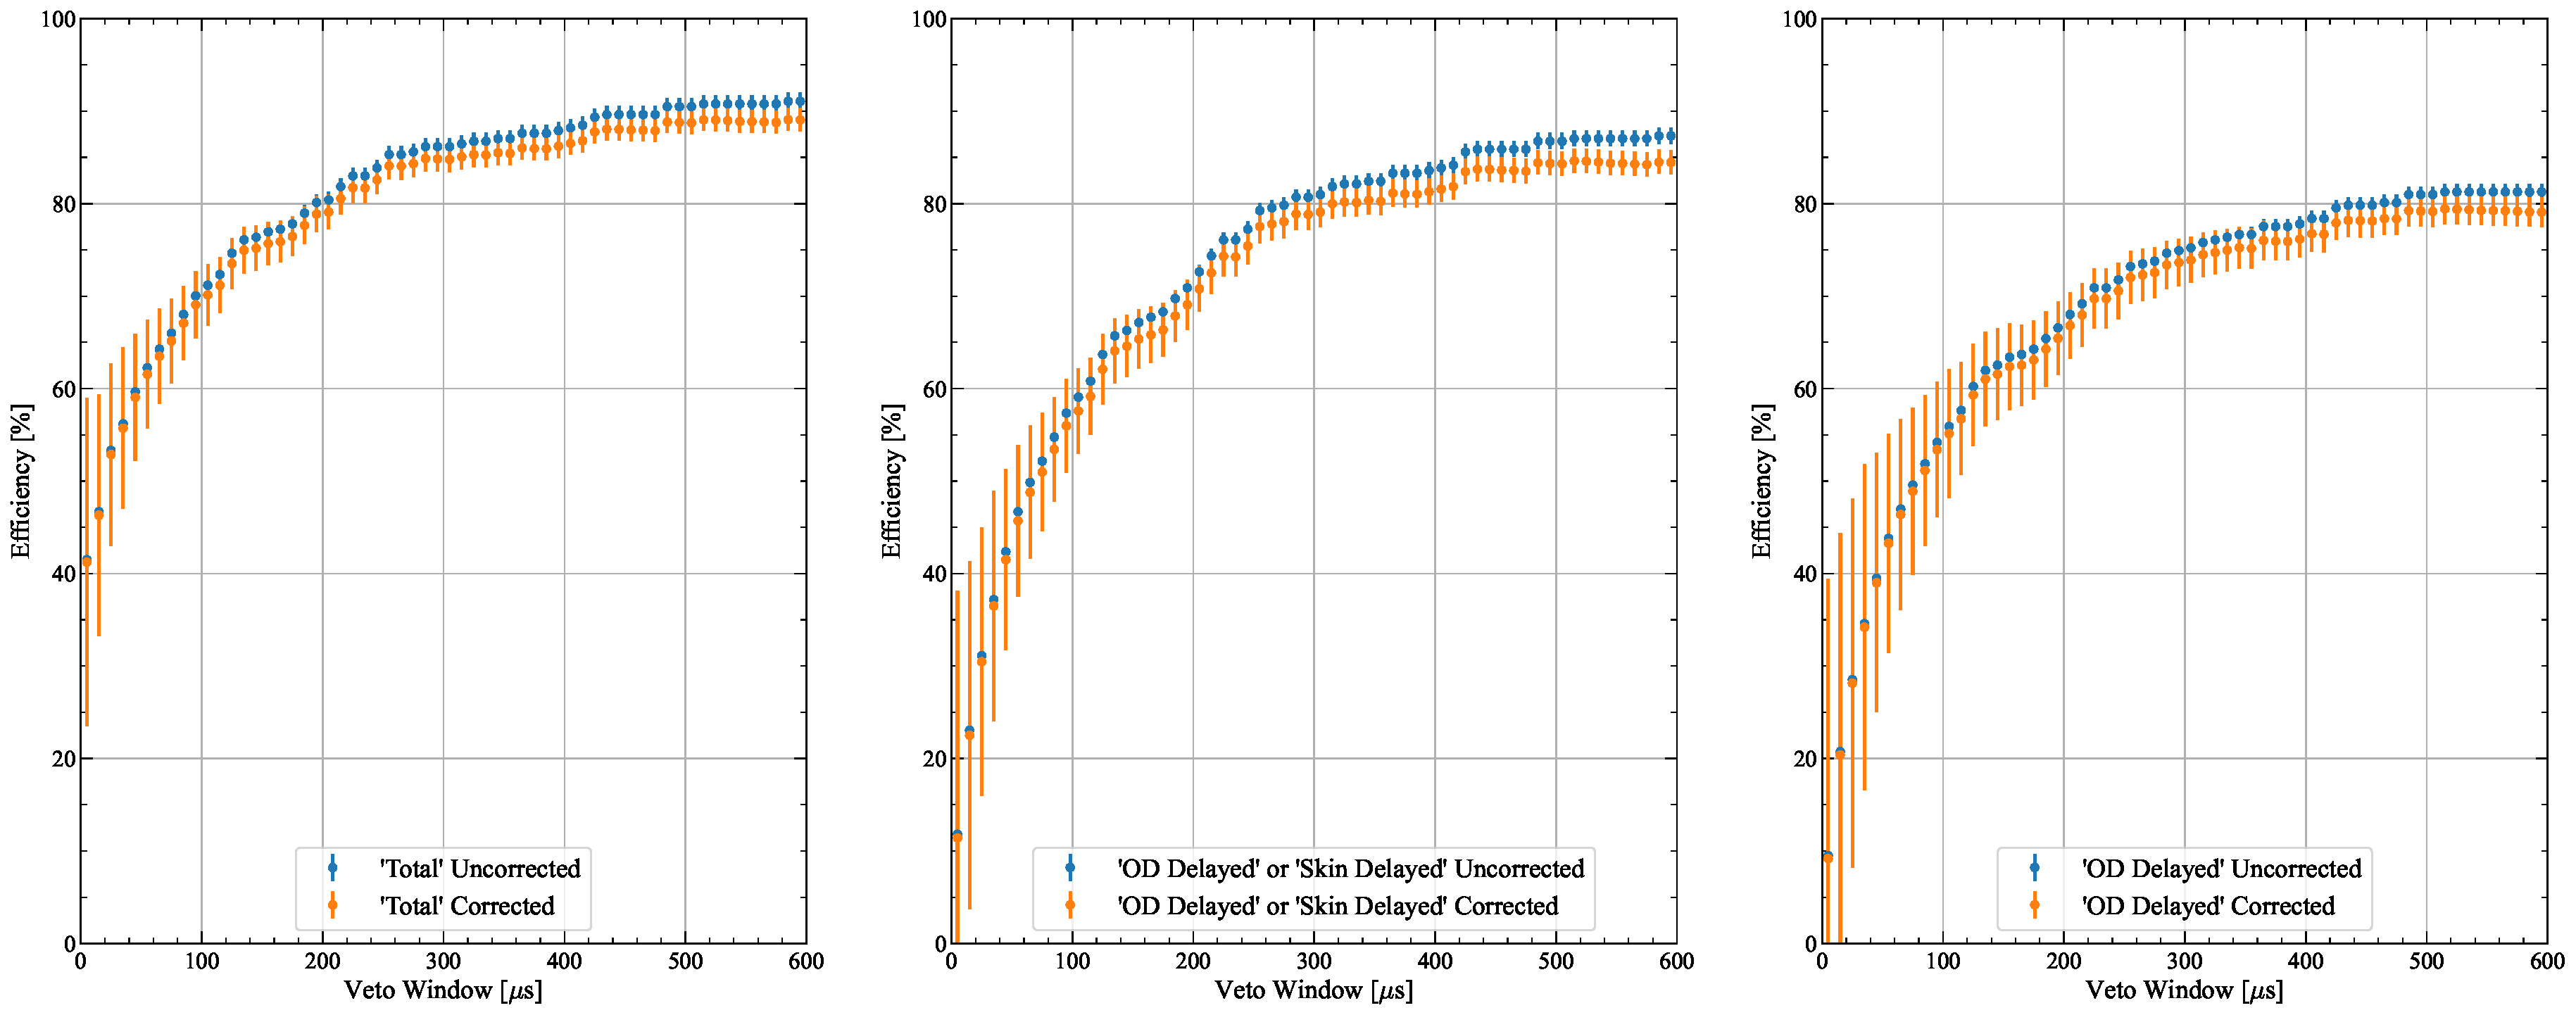
\includegraphics[width=\textwidth]{figures/VetoEfficiency/AccidentalCorrectionImpact.pdf}
	\caption{The impact of the accidental correction applied to the different veto efficiencies for the given windows of interest. AmLi data at a height of 700~mm in CSD1 has been used here as an example.}
	\label{fig:VetoEff/AccidentalImpact}
\end{figure}


\subsubsection{DD direct}
The DD calibration runs are from the October-2023 calibration period during the WS2024 science run, with run control operation name \textbf{DD Plasma}.
The runs used are; \lstinline{14631-14654}.
All files were processed with \lstinline{LZAP-5.8.0}.
The analysis for DD follows a logic similar to the AmLi described in \autoref{sec:VetoEff/AmLi_Efficiency}.
The cuts used for DD are listed in \autoref{tab:VetoEff/dd_efficiency_cuts}.
In addition to these cuts, an NR band cut was also applied.
It is important to note that this NR band is different to the one used for AmLi. The two different NR bands for the calibration sources is shown in \autoref{fig:VetoEff/SR3NRBands}.
%The band can be found on NERSC at \lstinline{/global/cfs/cdirs/lz/physics/NEST_Bands/SR3/20240313/Calibration}, if it has been moved, it can be recreated with the Woods parameters listed below;
The band was generated using the NEST, it can be recreated with the Woods parameters listed below;
\begin{lstlisting}[backgroundcolor = \color{lightgray}]
The Woods Function Fit Parameters for the Band Mean are:
[-19.937161961102728, 19.923601138859933,
0.0003111152850489644, 3.9306761416517557]

The Woods Function Fit Parameters for the 10% CL Line are:
[-17.635537023159518, 15.192184130700792,
0.000791717641575967, 3.813184578175848]

The Woods Function Fit Parameters for the 90% CL Line are:
[-32.02840007751605, 32.68367426603315,
-0.0006477294838326959, 4.157363202993382]
\end{lstlisting}
\begin{table}[!ht]
	\centering
	\caption{ALPACA-Core WS2024 cuts used on DD calibration data for determining the efficiency.}
	\begin{tabular}{|c|c|c|}
    \hline
	\textbf{Physics cuts}&\textbf{ S1 cuts}&\textbf{S2 cuts} \\
	\hline
	Single scatter & S2 width vs drift time & S1 prominence cut \\
	S1 and S2 threshold & Narrow S2 & Stinger event cut \\
	Fiducial Volume & S2 rise time & S1 TBA vs drift time \\
	& S2 early peak & S1 HSC cut \\
	& S2 XY quality & S1 shape \\
	& S2 TBA (above-anode gas) & S1 photon timing \\
    \hline
	\end{tabular}
	\label{tab:VetoEff/dd_efficiency_cuts}
\end{table}
\subsubsection{DD accidental correction}
The DD calibration data was also corrected for accidentals. The same method was used which was previously discussed in \autoref{sec:VetoEff/AmLiAccCorrection}. The correction factors used as a function of veto window can be seen in \autoref{fig:VetoEff/DDAccCorrectionParameters}.
The impact of the accidental corrections on the DD veto efficiency can be seen in \autoref{fig:VetoEff/DDAccCorrectionImpact_P0}.

\begin{figure}[!ht]
	\centering
	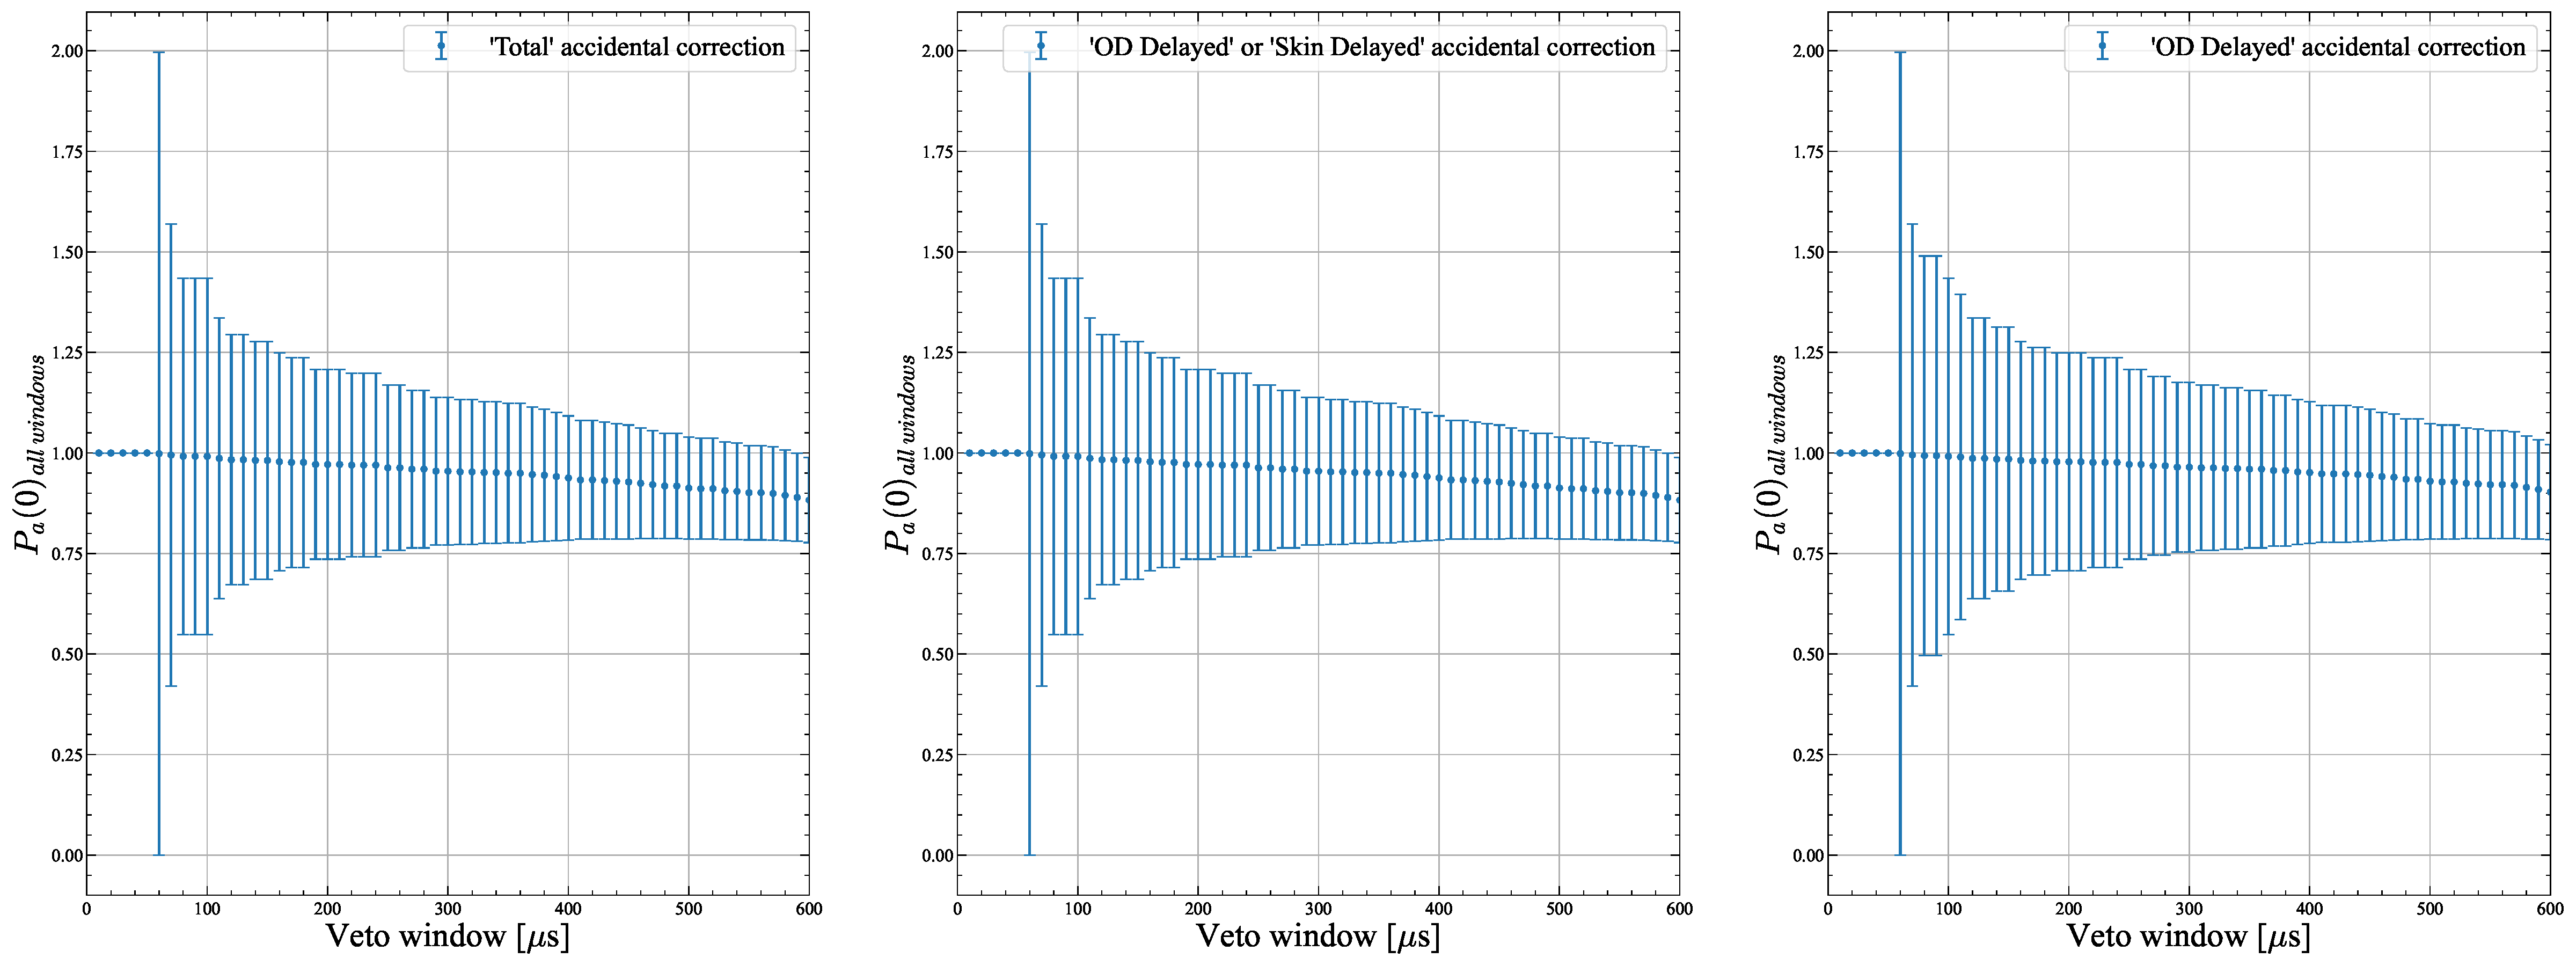
\includegraphics[width=\textwidth]{figures/VetoEfficiency/DDAccCorrectionImpact_P0.pdf}
	\caption{$P_a(>0)_{all\:window}$ DD Accidental correction factors for varying veto window size for different windows of interest.}
	\label{fig:VetoEff/DDAccCorrectionImpact_P0}
\end{figure}

\begin{figure}[!ht]
	\centering
	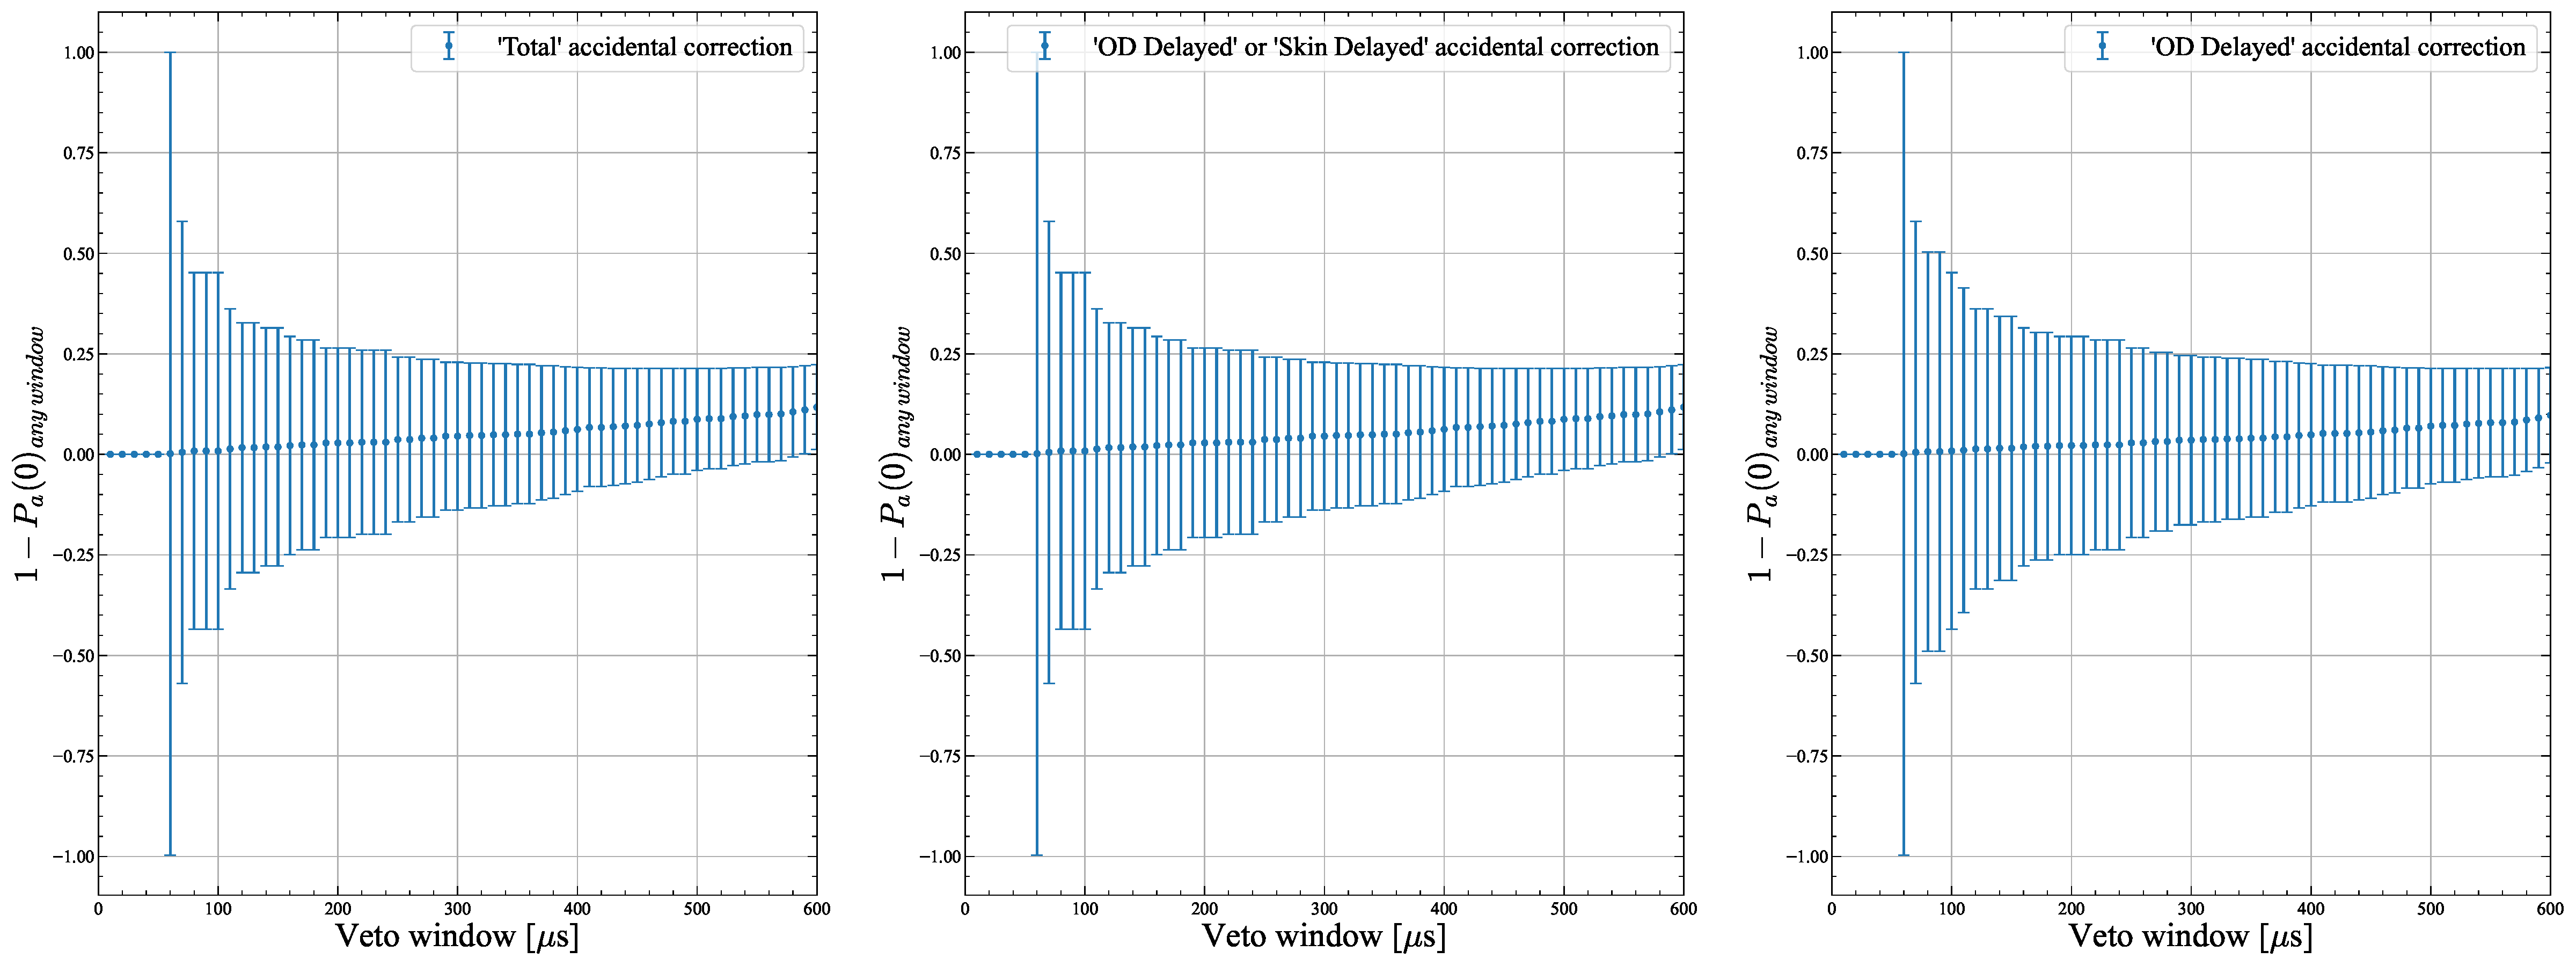
\includegraphics[width=\textwidth]{figures/VetoEfficiency/DDAccCorrectionImpact_1-P0.pdf}
	\caption{$1-P_a(>0)_{any\:window}$DD Accidental correction factors for varying veto window size for different windows of interest.}
	\label{fig:VetoEff/DDAccCorrectionImpact_1-P0}
\end{figure}

\begin{figure}[!ht]
	\centering
	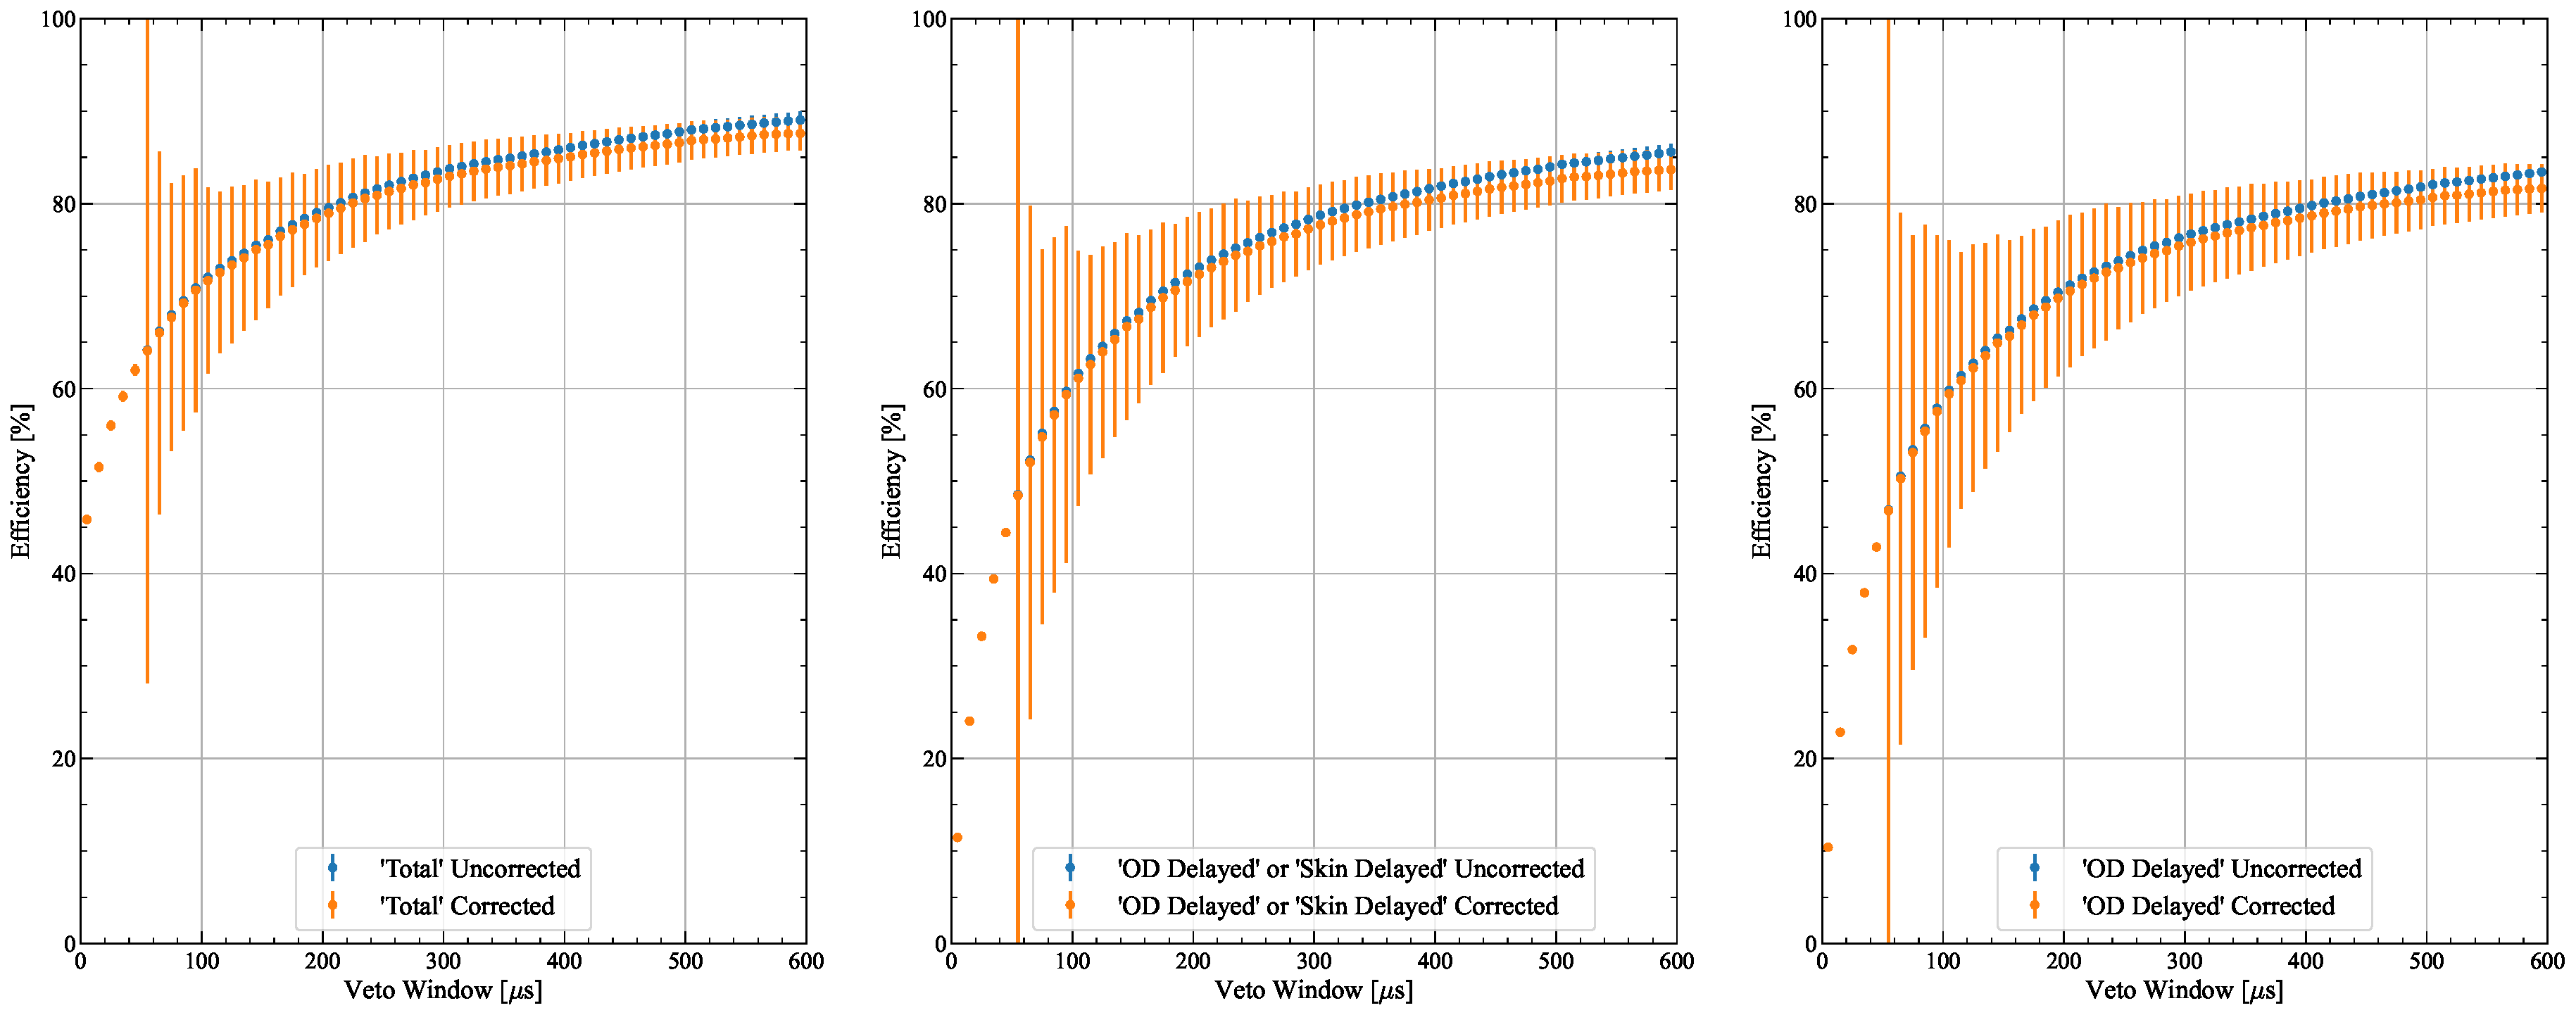
\includegraphics[width=\textwidth]{figures/VetoEfficiency/DDAccCorrectionParameters.pdf}
	\caption{The impact of the accidental correction applied to the different veto efficiencies for the given windows of interest.}
	\label{fig:VetoEff/DDAccCorrectionParameters}
\end{figure}

\subsection{Simulated neutrons from calibration sources}
AmLi and DD were simulated using \lstinline{BACCARAT-6.3.5} and \lstinline{LZLAMA-3.5.3} versions.
On each set of simulation, the cuts listed in \autoref{tab:VetoEff/calibration_simulation_efficiency_cuts} were used.
\begin{table}[!ht]
	\centering
	\caption{ALPACA-Core WS2024 cuts used on AmLi and DD simulations for determining the efficiency.}
	\begin{tabular}{|c|}
    \hline
		\textbf{Physics cuts}              \\
		\hline
		Single scatter            \\
		S1 and S2 threshold       \\
		Fiducial Volume           \\
		CSD Selection (AmLi Only) \\
        \hline
	\end{tabular}
	\label{tab:VetoEff/calibration_simulation_efficiency_cuts}
\end{table}
No accidental correction was applied to the simulation data as there are no accidental gammas or neutrons present in the simulation.
How these compare to the data measurements are shown in \autoref{fig:VetoEff/AmLiIneffPlots}-\ref{fig:VetoEff/DDIneffPlots}.
%More detailed plots on how the calibration simulations compare to calibration data is in \autoref{sec:VetoEff/simulation_improvements}.
%TODO: Should I make the comparison between data and sim with respect to what Alberto did
\begin{figure}[!ht]
	\centering
	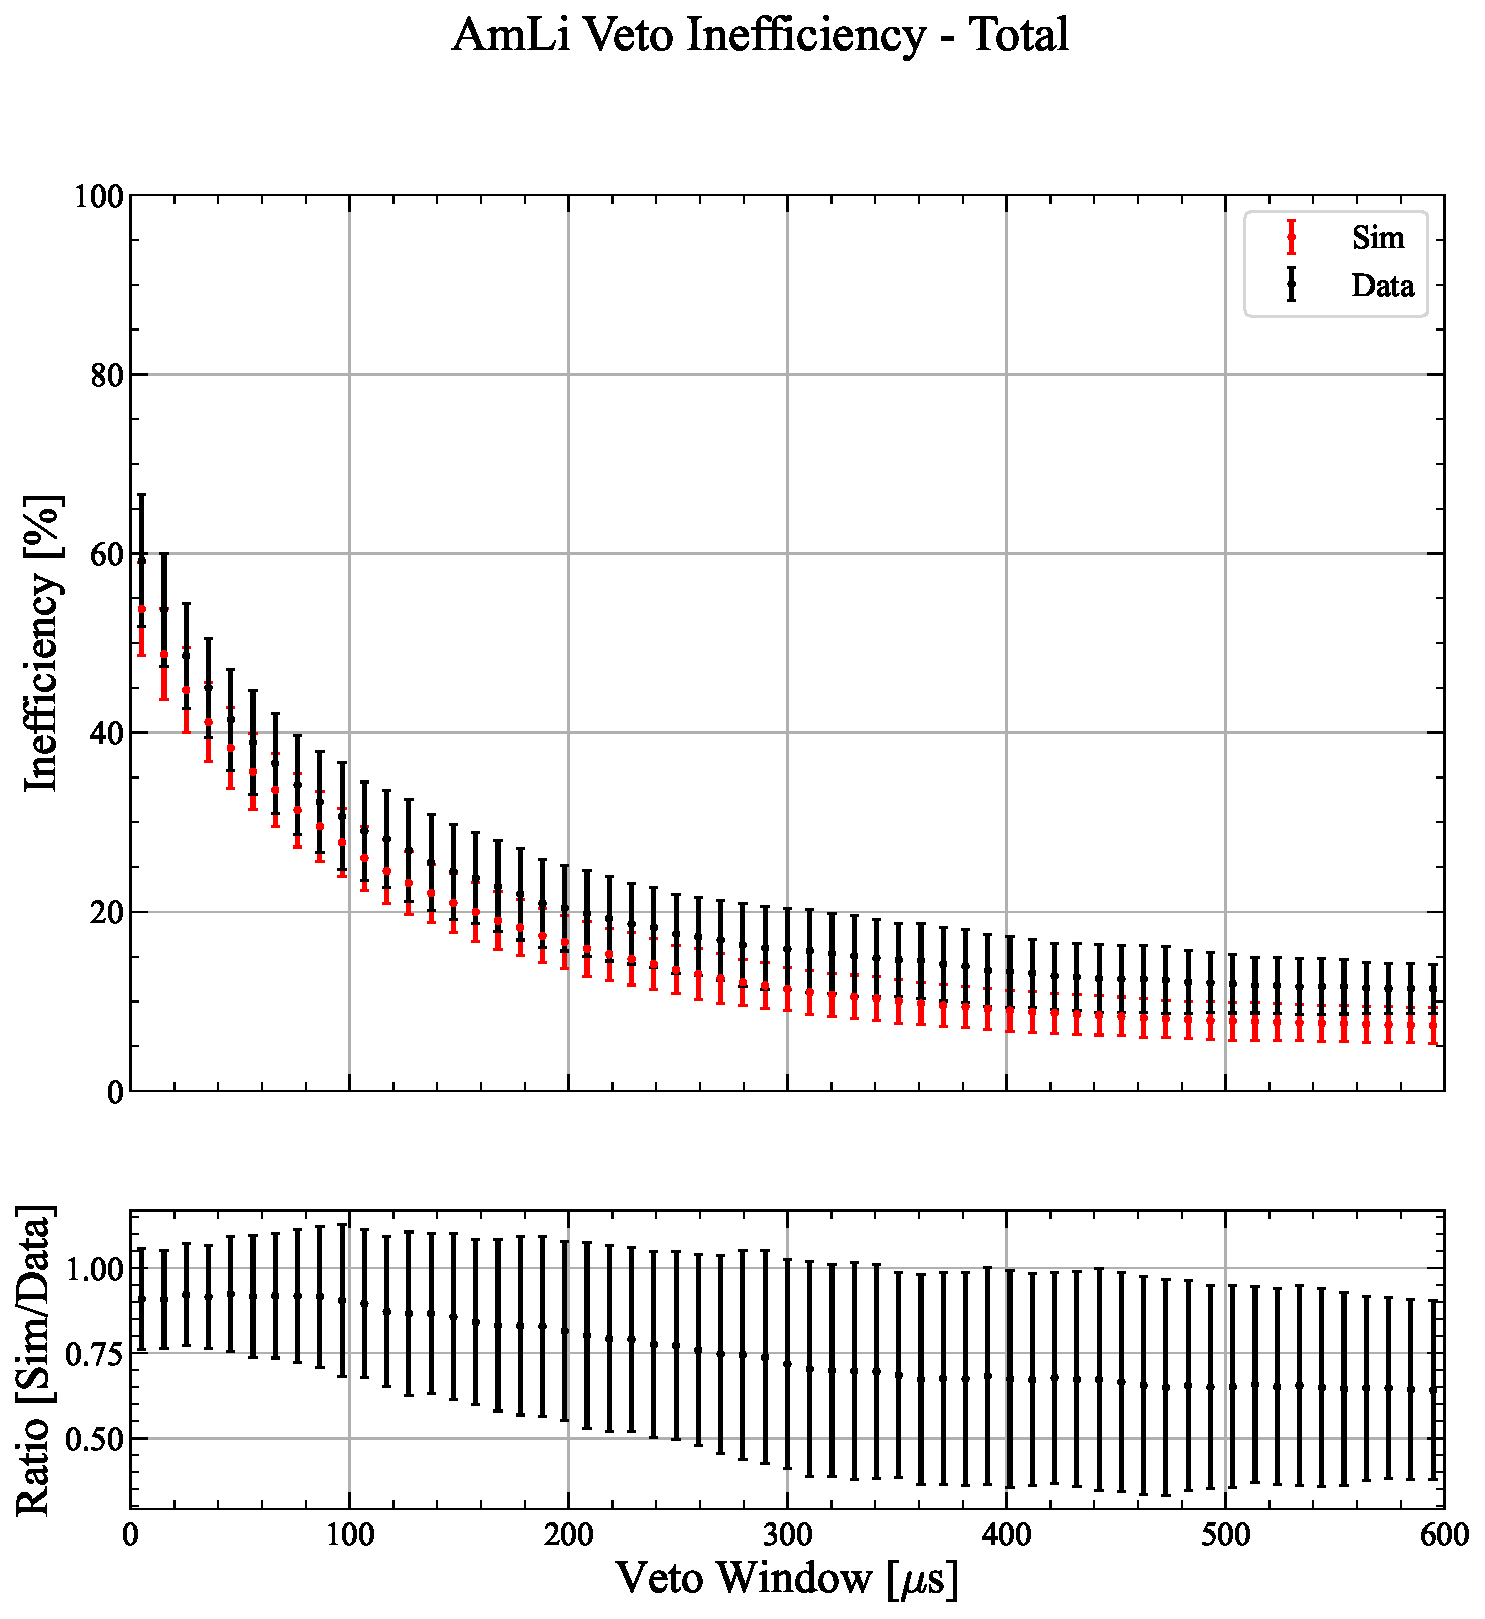
\includegraphics[width=.3\textwidth]{figures/VetoEfficiency/InEff_AmLi_Total_Avg_Ratio.pdf}\hfill
	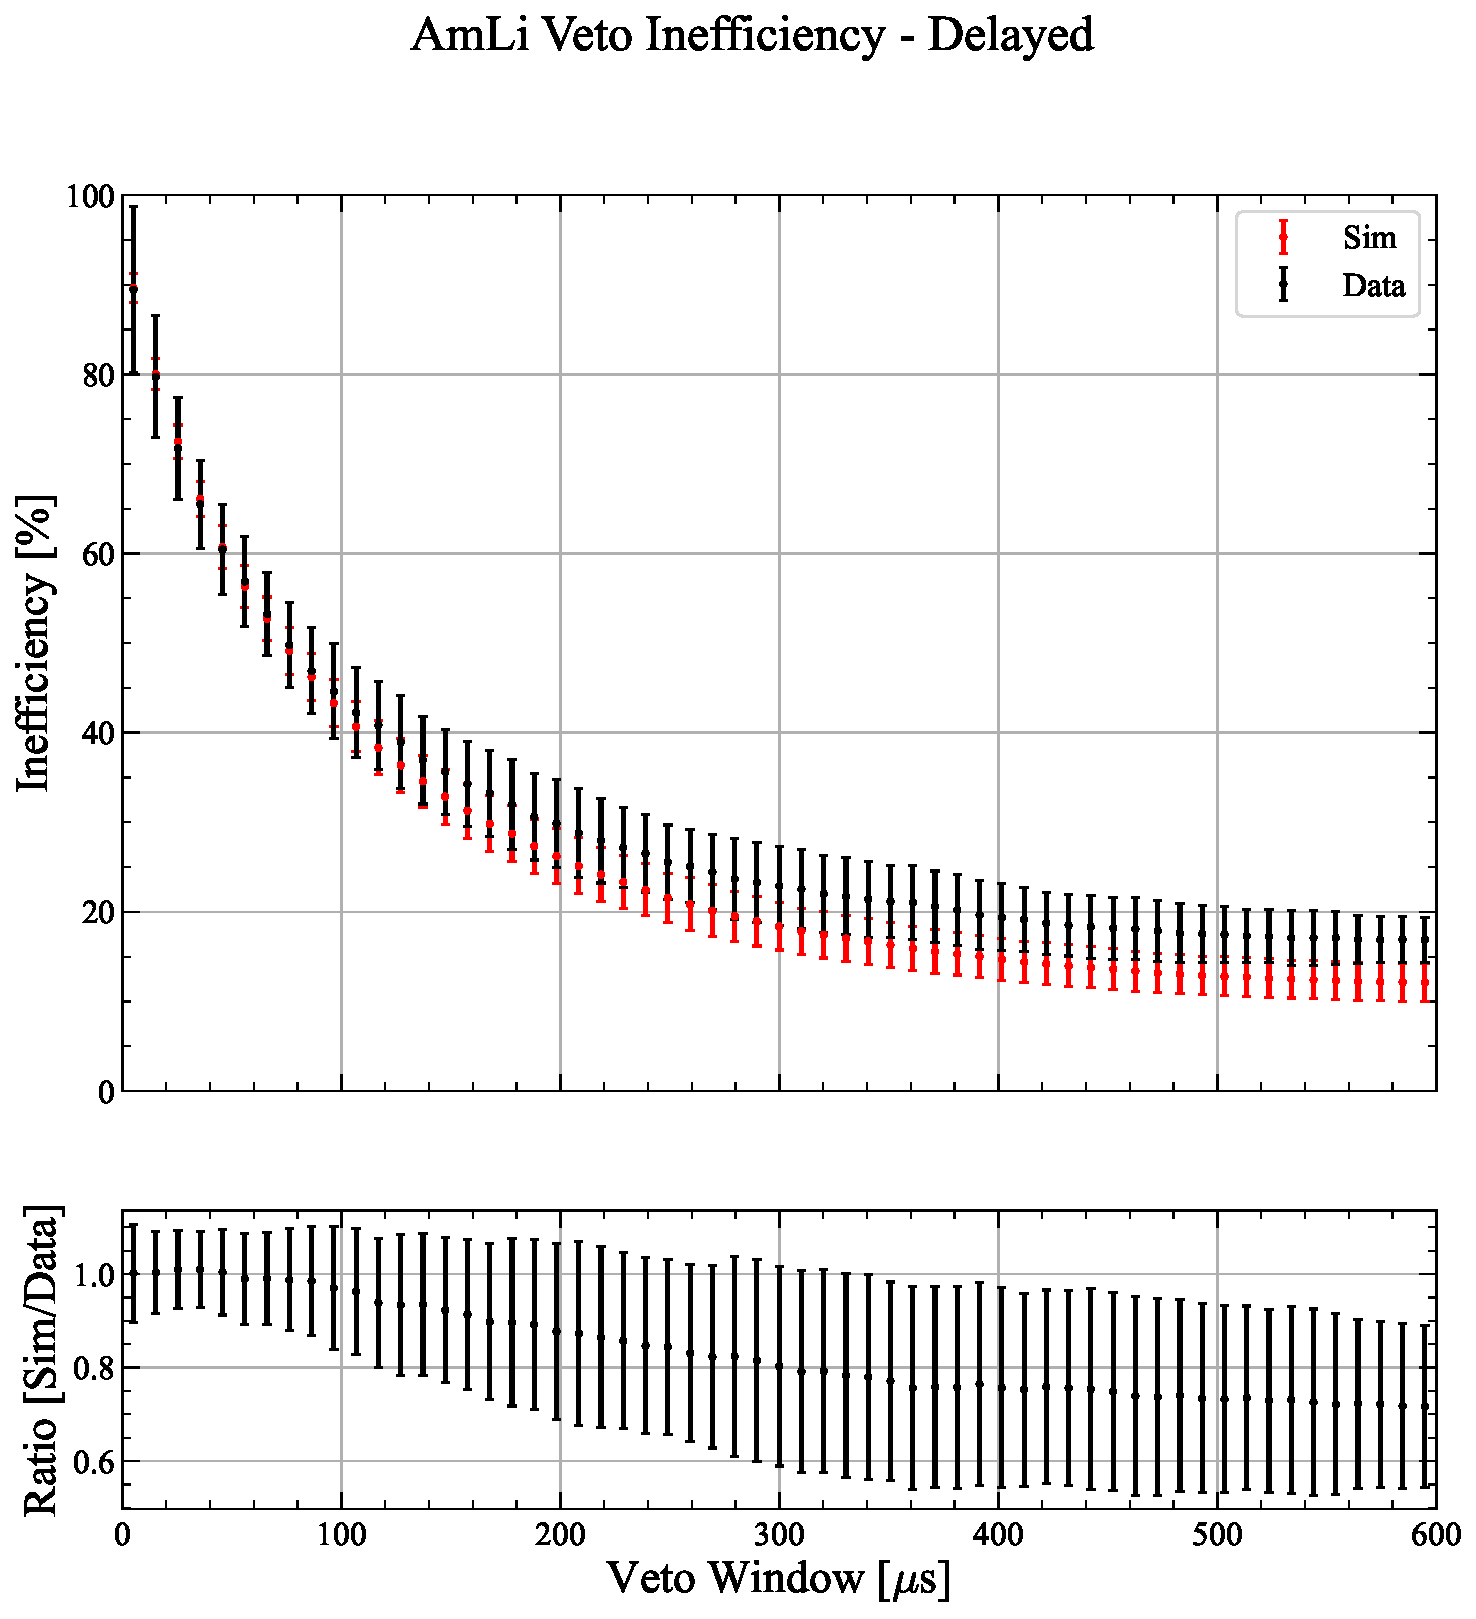
\includegraphics[width=.3\textwidth]{figures/VetoEfficiency/InEff_AmLi_Delayed_Avg_Ratio.pdf}\hfill
	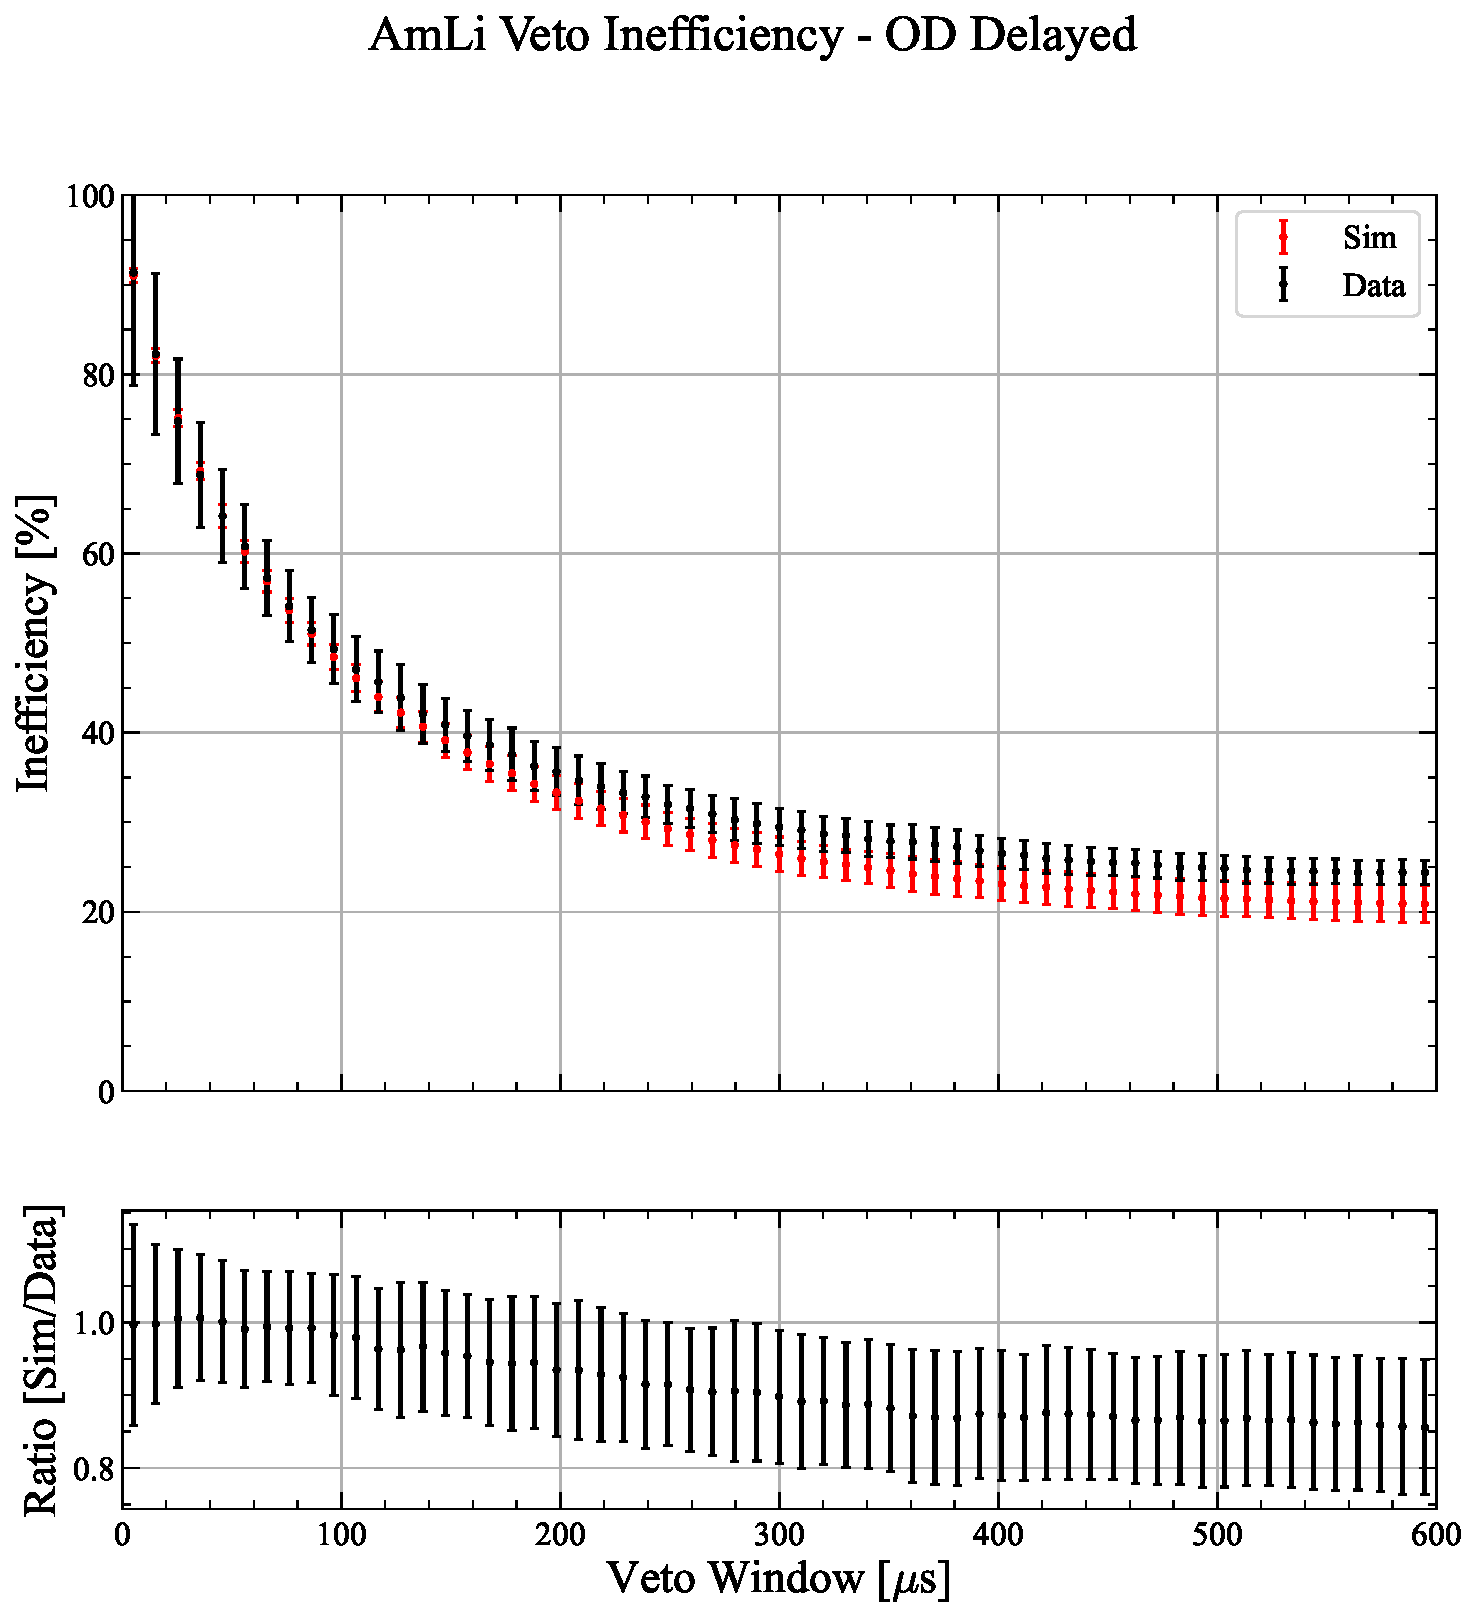
\includegraphics[width=.3\textwidth]{figures/VetoEfficiency/InEff_AmLi_ODDelayed_Avg_Ratio.pdf}
	\caption{Inefficiency plots for AmLi, comparing simulations to data.
		Left: Total. Middle: Delayed Only. Right: OD Delayed.\\
		In each case, the average from all CSD positions are used.}
	\label{fig:VetoEff/AmLiIneffPlots}
\end{figure}

\begin{figure}[!ht]
	\centering
	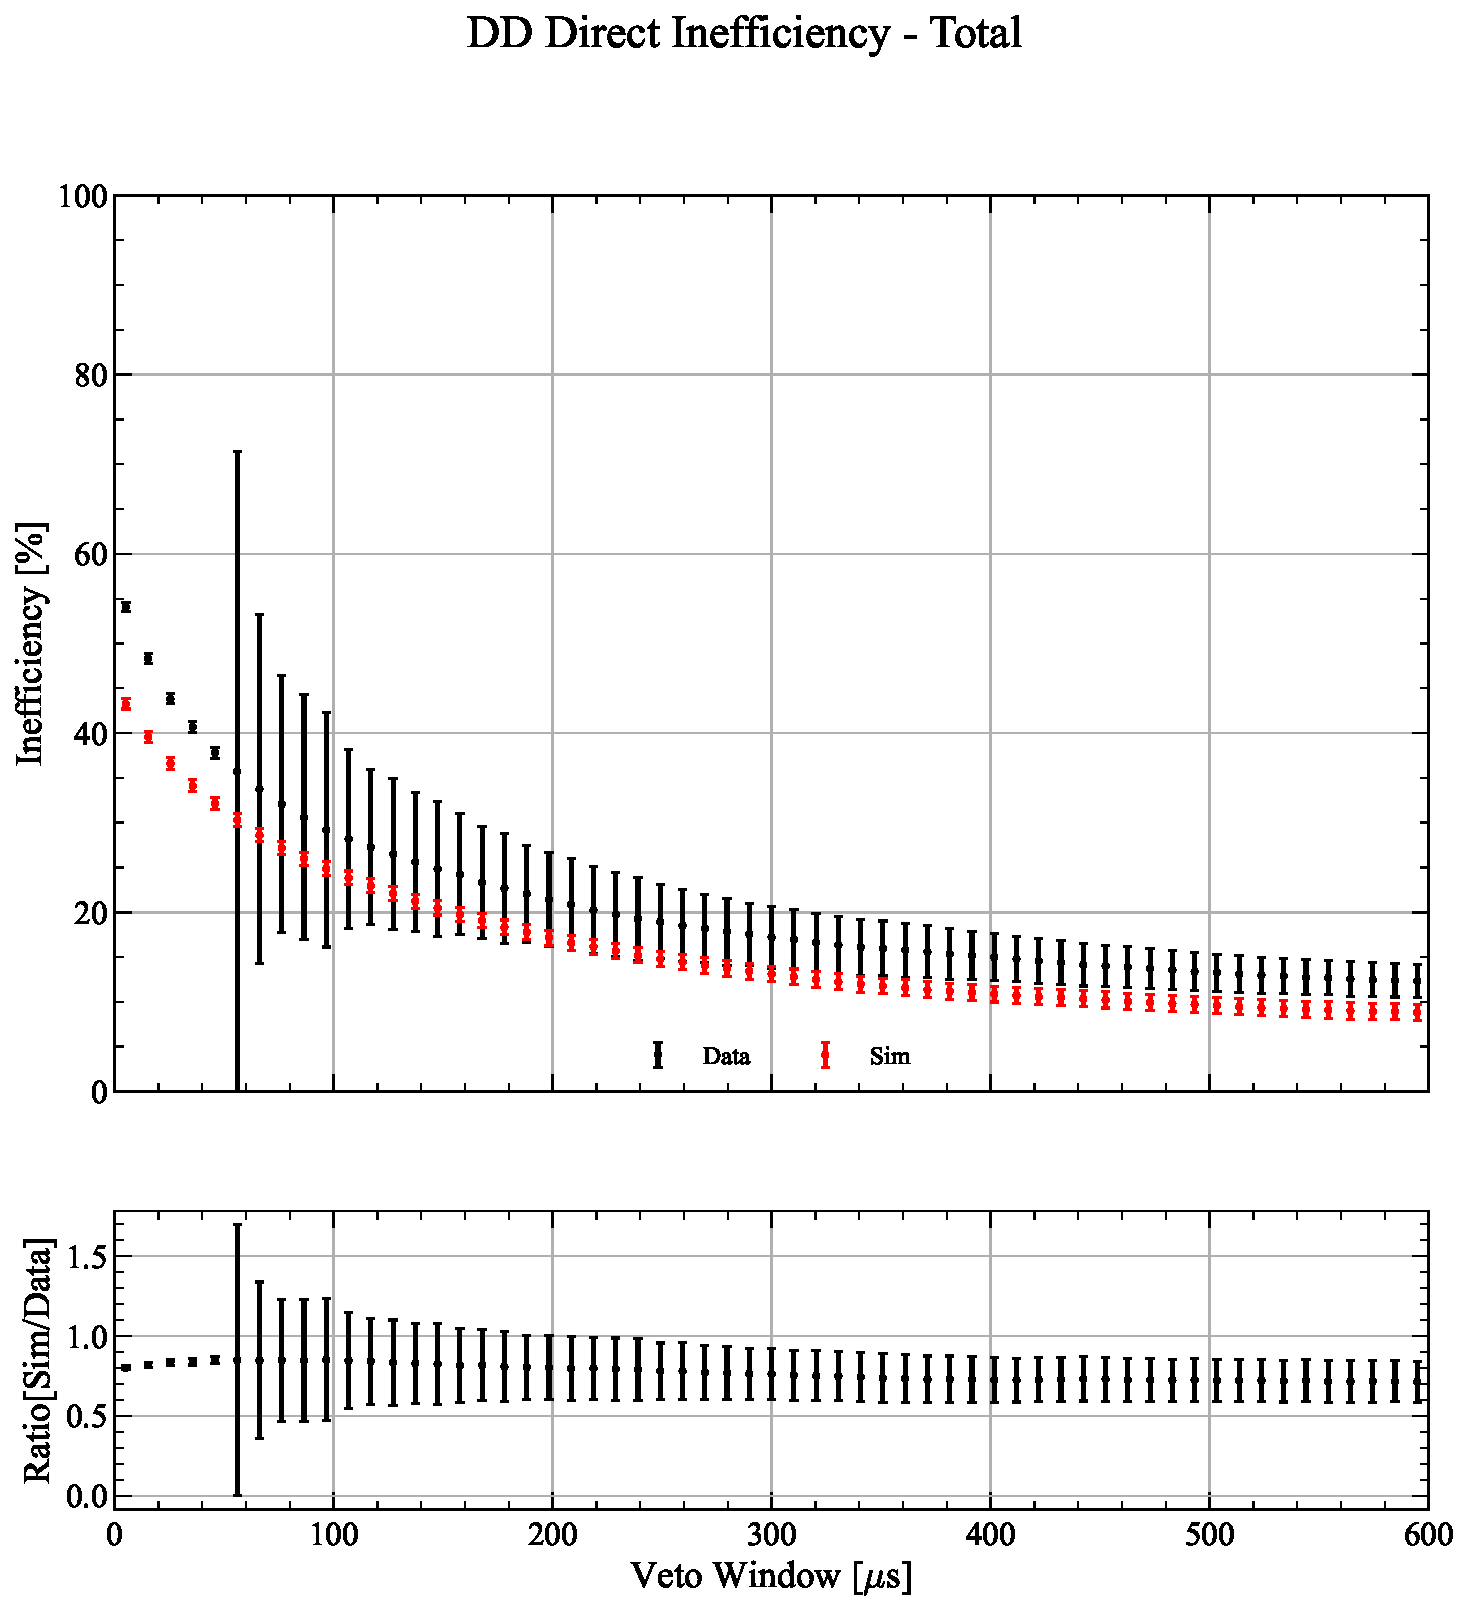
\includegraphics[width=.3\textwidth]{figures/VetoEfficiency/InEff_DDDirect_Total_Ratio.pdf}\hfill
	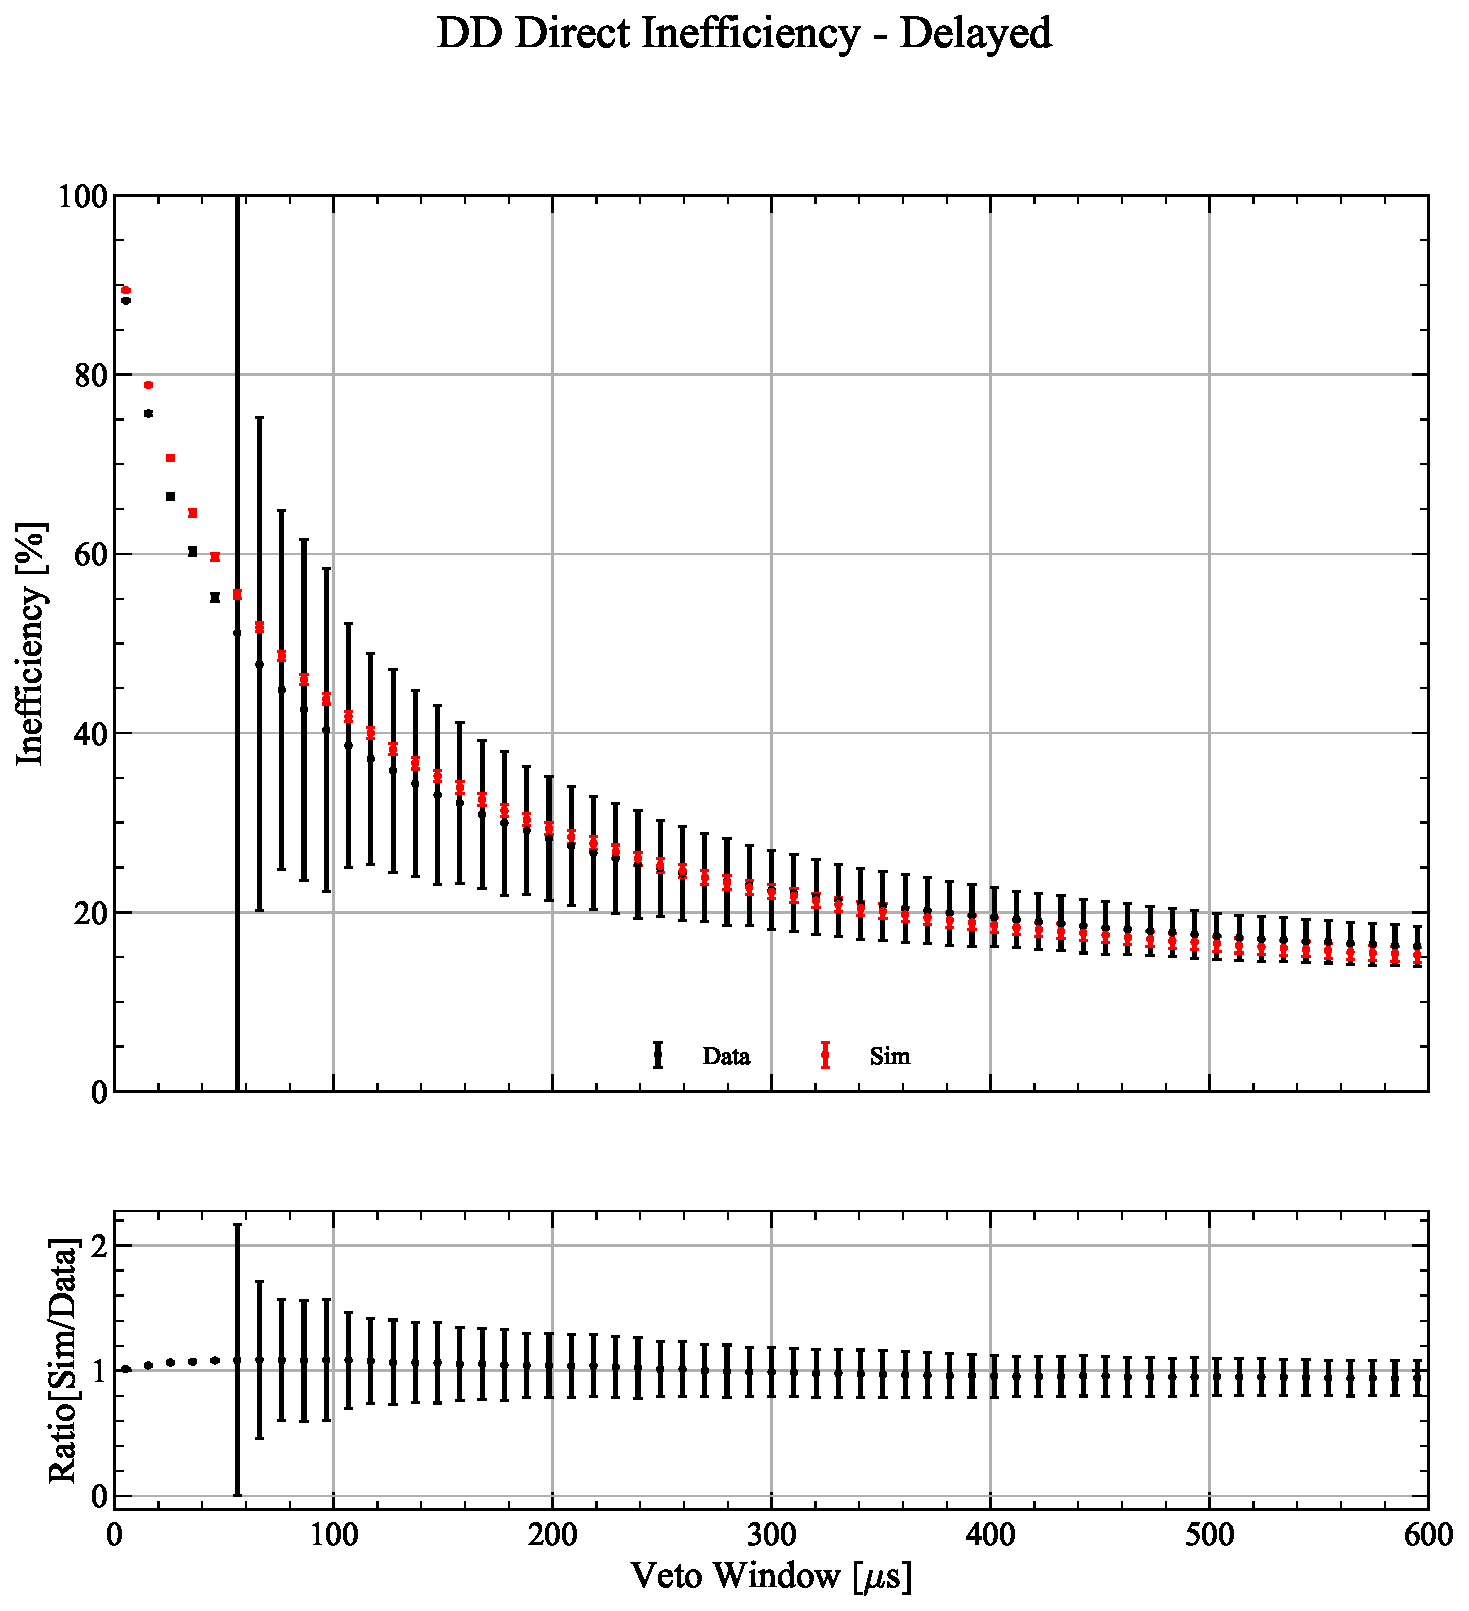
\includegraphics[width=.3\textwidth]{figures/VetoEfficiency/InEff_DDDirect_Delayed_Ratio.pdf}\hfill
	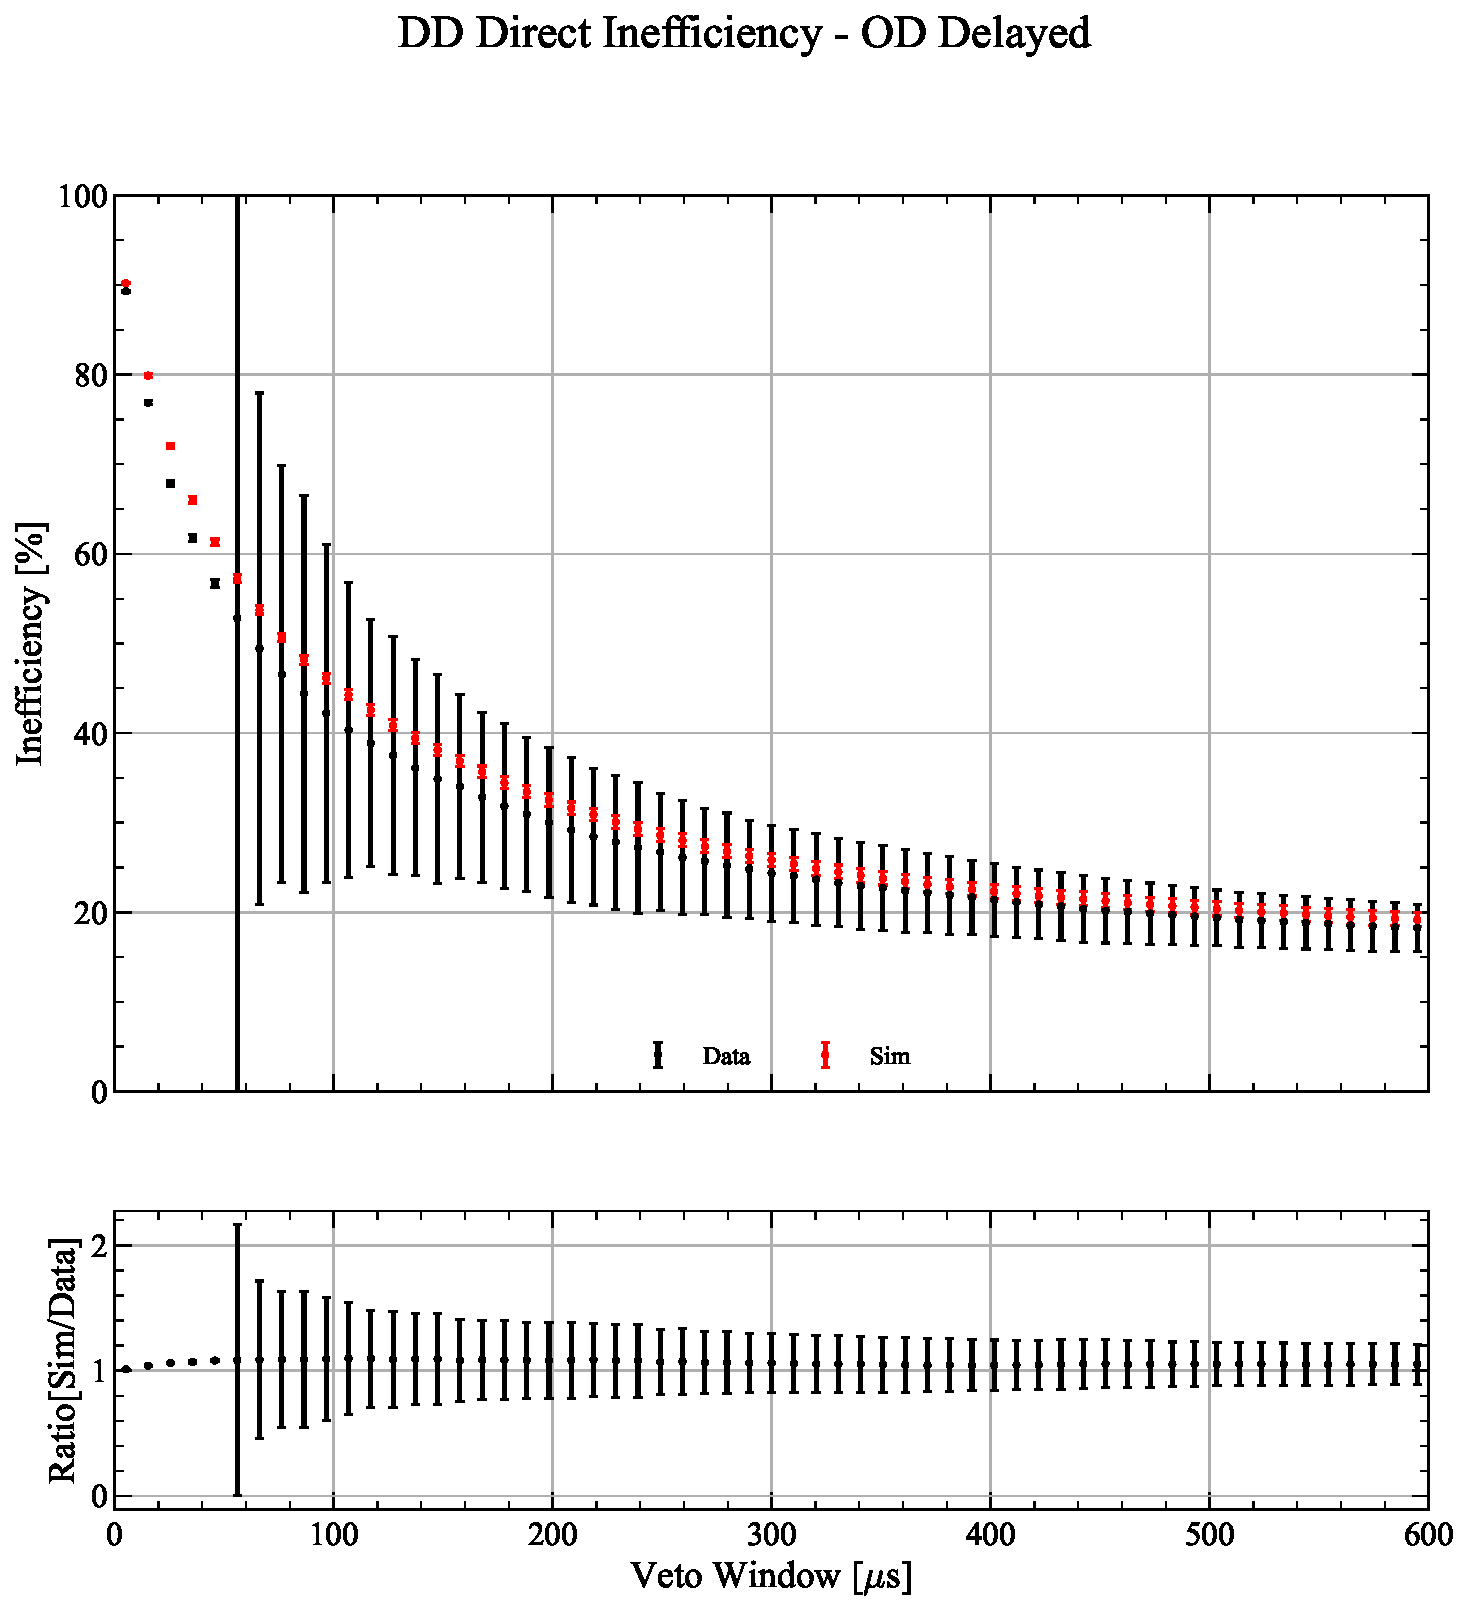
\includegraphics[width=.3\textwidth]{figures/VetoEfficiency/InEff_DDDirect_ODDelayed_Ratio.pdf}
	\caption{\centering Inefficiency plots for DD, comparing simulations to data.\\ Left: Total. Middle: Delayed Only. Right: OD Delayed.}
	\label{fig:VetoEff/DDIneffPlots}
\end{figure}

\subsection{Background neutrons}
The detector-NR simulations were simulated as part of the official production of SR3-BG. Each of the 644 components were simulated using BACCARAT-6.3.5 and LZLAMA-3.5.3 versions.
The cuts listed in \autoref{tab:VetoEff/detector_nr_simulation_efficiency_cuts} were applied.
The efficiency of tagging neutrons from Uranium Spontaneous Fission (USF) and ($\alpha$,n) events are shown in \autoref{fig:VetoEff/detector_nr_efficiency}.
Also shown is the total efficiency.

\begin{table}[!ht]
	\centering
	\caption{ALPACA-Core WS2024 cuts used on Detector-NR simulations for determining the efficiency. Each cut is from WS2024-cuts-v3.}
	\begin{tabular}{|c|}
    \hline
		\textbf{Physics cuts}        \\
		\hline
		Single scatter      \\
		S1 and S2 threshold \\
		Fiducial Volume\\
        \hline
	\end{tabular}
	\label{tab:VetoEff/detector_nr_simulation_efficiency_cuts}
\end{table}

\begin{figure}[!ht]
	\centering
	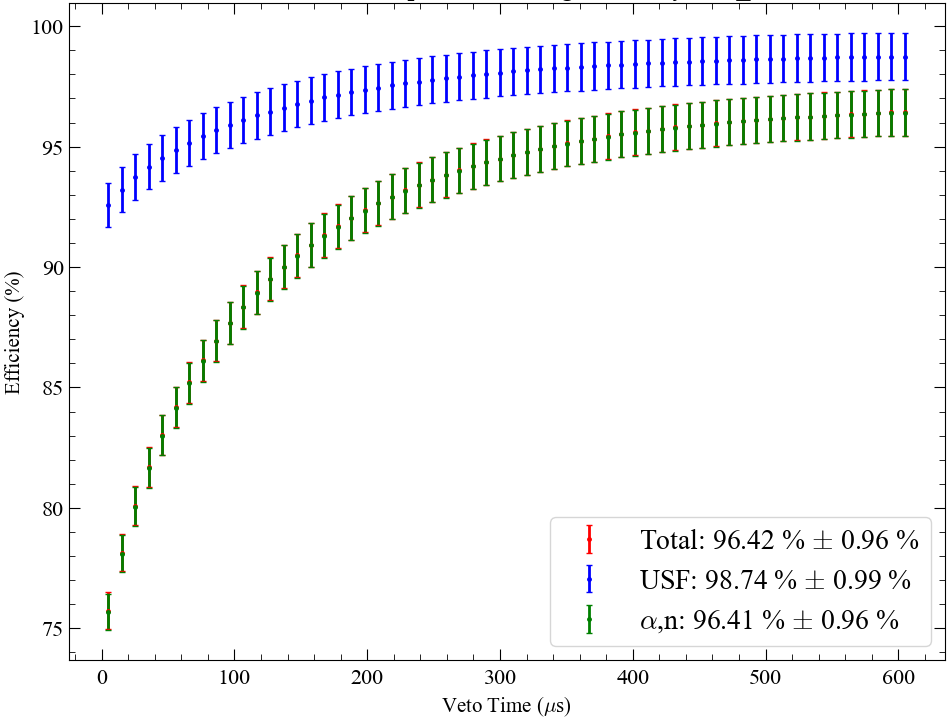
\includegraphics[width=0.8\textwidth]{figures/VetoEfficiency/det_nr_efficiency.png}
	\caption{Efficiency for tagging a neutron on Detector-NR simulations.}
	\label{fig:VetoEff/detector_nr_efficiency}
\end{figure}

\clearpage
\subsection{Background neutron efficiency from data}\label{sec:VetoEff/BkgNeutronEff}
The neutron veto efficiency from each calibration source from data and simulation is shown in \autoref{fig:VetoEff/efficiency_summary}.
Also shown is the efficiency from simulated background neutrons.
The Z-position of each point is calculated from the \lstinline{mean(driftTime)} of events which pass the selection.
For the Detector-NR, the events were split up into Z-sections by the following;
\begin{lstlisting}[backgroundcolor = \color{lightgray},language = Python]
def SR3ZThirds_Cut(driftTime_us: float, position='top'):
    if position == 'top':
        return ((driftTime_us < 350.) & (driftTime_us > 71.))
    elif position == 'mid':
        return ((driftTime_us < 700.) & (driftTime_us > 350.))
    elif position == 'bot':
        return ((driftTime_us < 1030.) & (driftTime_us > 700.))
\end{lstlisting}
This \lstinline{driftTime} splitting was performed so that comparing to calibration points was easier, but in evaluating the total efficiency, it was not used.
Shown in \autoref{tab:VetoEff/final_veto_efficiency} are the veto efficiencies of all calibration sources for both simulations and data.
The value of importance is the background neutron efficiency, $\epsilon_{\textrm{bg data}}$, or inefficiency, $\zeta_{\textrm{bg data}}$.
There are a number of ways in which this can be calculated, which are described below.
The option 2 was used for the final WS2024 result, of 7.8$\pm$4.3\%; or quote as 8$\pm$4.
\autoref{tab:VetoEff/efficiency_options} contains the results of each approach.
\paragraph{Option 1}:
The average simulation calibration efficiency was taken, so the mean of AmLi (92.8\%) and DD (91.8\%), resulted in an average efficiency of 92.3\%.
The average data calibration efficiency was taken, so the mean of AmLi (88.6\%) and DD (87.7\%), resulted in an average of 88.2\%.
The ratio, $\Delta$, of the simulation calibrations and the data calibration can then be used as a scaling factor on the simulation background.
This process is expressed in \autoref{eqn:VetoEff/:efficiency_option1}, and gives an efficiency of 92.1\%.
In this case, the uncertainty is 4.5\%, made up from a statistical error from the simulations (0.96\%), and 4.3 from the scaling.
\begin{align}
	\epsilon_{\textrm{cal. data}} & = \frac{\epsilon_{\textrm{data DD}} + \epsilon_{\textrm{data AmLi}}}{2} \\
	\epsilon_{\textrm{cal. sims}} & = \frac{\epsilon_{\textrm{sims DD}} + \epsilon_{\textrm{sims AmLi}}}{2} \\
	\Delta                        & = \frac{\epsilon_{\textrm{cal. data}}}{\epsilon_{\textrm{cal. sims}}}   \\
	\epsilon_{\textrm{bg data}}   & = \Delta \times \epsilon_{\textrm{bg sims}}
	\label{eqn:VetoEff/:efficiency_option1}
\end{align}

\paragraph{Option 2}:
The average simulation calibration efficiency was taken, mean of AmLi (92.8\%) and DD (91.8\%) resulted in an average efficiency of 92.3\%.
The average data calibration efficiency was taken, mean of AmLi (88.6\%) and of DD (87.7\%), resulted in an average efficiency of 88.2\%.
The difference, $\Lambda$, between the simulation calibrations and the data calibrations can then be used as a systematic uncertainty on the simulation backgrounds.
This process is expressed in \autoref{eqn:VetoEff/:efficiency_option2}, and gives an efficiency of 92.2\%.
In this case, the uncertainty is 4.3\%, made up from a statistical error from the simulations (0.96\%), and 4.22 from the subtraction.

\begin{align}
	\epsilon_{\textrm{cal. data}} & = \frac{\epsilon_{\textrm{data DD}} + \epsilon_{\textrm{data AmLi}}}{2} \\
	\epsilon_{\textrm{cal. sims}} & = \frac{\epsilon_{\textrm{sims DD}} + \epsilon_{\textrm{sims AmLi}}}{2} \\
	\Lambda                       & = \epsilon_{\textrm{cal. sims}} - \epsilon_{\textrm{cal. data}}         \\
	\epsilon_{\textrm{bg data}}   & = \epsilon_{\textrm{bg sims}} - \Lambda
	\label{eqn:VetoEff/:efficiency_option2}
\end{align}

\paragraph{Option 3}:
The average simulation calibration inefficiency was taken, the mean of AmLi ($100 - 92.8 = 7.2$\%) and DD ($100 - 91.8 = 8.3$\%), resulted in an inefficiency of 7.7\%.
The average data calibration inefficiency was taken, the mean of AmLi (11.5\%) and DD (12.3\%), resulted in an average inefficiency of 11.9\%.
The ratio, $\Delta$, of the simulation calibrations and the data calibration can then be used as a scaling factor on the simulation background.
This process is expressed in \autoref{eqn:VetoEff/:efficiency_option3}, and gives an inefficiency of 5.5.
In this case, the uncertainty is 2.8\%, made up from a statistical error from the simulations (0.96\%), and 1.8 from the subtraction.

\begin{align}
	\zeta_{\textrm{cal. data}} & = 100 - \frac{\epsilon_{\textrm{data DD}} +\epsilon_{\textrm{data AmLi}}}{2}  \\
	\zeta_{\textrm{cal. sims}} & = 100 - \frac{\epsilon_{\textrm{sims DD}} + \epsilon_{\textrm{sims AmLi}}}{2} \\
	\Delta                     & = \frac{\zeta_{\textrm{cal. data}}}{\zeta_{\textrm{cal. sims}}}               \\
	\zeta_{\textrm{bg data}}   & = \zeta_{\textrm{bg sims}} \times \Delta
	\label{eqn:VetoEff/:efficiency_option3}
\end{align}

\begin{table}[!ht]
	\centering
	\caption{Summary of veto efficiencies. The Detector-NR Data value assumes that option 2 is used.}
	\begin{tabular}{|c|c|c|}
    \hline
		\textbf{Source}& \textbf{Simulation}& \textbf{Data}\\ 
        \hline
		AmLi (average) & 92.8$\pm$2.0\% & 88.6$\pm$2.7\% \\
		DD (Direct)    & 91.8$\pm$1.0\% & 87.7$\pm$1.8\% \\
		Detector-NR    & 96.4$\pm$1.0\% & 92.2$\pm$4.3\\
        \hline
	\end{tabular}
	\label{tab:VetoEff/final_veto_efficiency}
\end{table}

\begin{table}[!ht]
	\caption{Summary of veto efficiencies and inefficiencies as determined from each approach discussed in \autoref{sec:VetoEff/BkgNeutronEff}.}
	\centering
	\begin{tabular}{|c|c|c|}
		\hline
        \textbf{Option} & \textbf{Efficiency}& \textbf{Inefficiency} \\ 
        \hline
		No. 1  & 92.1$\pm$4.5 & 7.9$\pm$4.5  \\
		No. 2  & 92.2$\pm$4.3 & 7.8$\pm$4.3  \\
		No. 3  & 94.5$\pm$2.8 & 5.5$\pm$2.8 \\
        \hline
	\end{tabular}
	\label{tab:VetoEff/efficiency_options}
\end{table}

\begin{figure}[!ht]
	\centering
	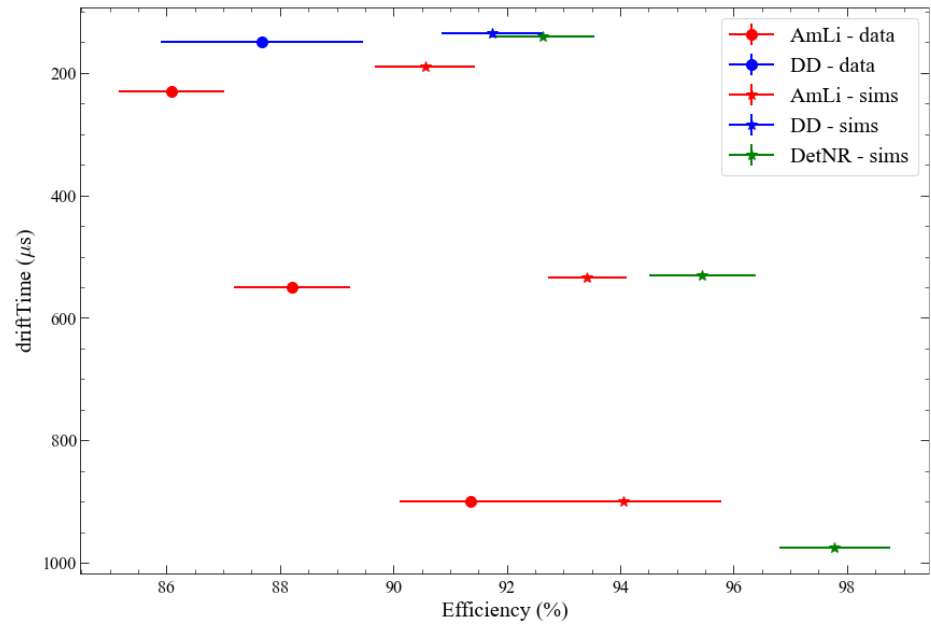
\includegraphics[width=0.8\textwidth]{figures/VetoEfficiency/efficiency_summary.png}
	\caption{Summary of efficiency from all simulations and calibration sources.
		The CSD sources are averaged at each height.
		Circle marks are from data.
		Start marks are from simulations.
		The \lstinline{driftTime} is defined as when \lstinline{mean(driftTime)} of events which pass all other cuts.
	}
	\label{fig:VetoEff/efficiency_summary}
\end{figure}

\section{Veto efficiency and the WIMP search}\label{sec:VetoEff4WIMPSearch}
\textcolor{red}{ToDo Need to talk about how the neutron efficiency is used in the WS result?}